% !TeX spellcheck = en_GB
\chapter{Computational Properties of Multi-Compartment LIF Neurons}
\label{chp:nlif}

\vspace{30pt}

\begin{OpeningQuote}
It may well be that certain nerve pulse combinations will stimulate a given neuron not simply by virtue of their number but also by virtue of the spatial relations of the synapses to which they arrive. This is, one may have to face situations in which there are, say, hundreds of synapses on a single nerve cell, and the combinations of stimulations on these that are effective [...] are characterised not only by their number, but also by their coverage of certain special regions on that neuron [...], by the spatial relations of such regions to each other, and by even more complicated quantiative and geometrical relationships that might be relevant.
\OpeningQuoteSource{John von Neumann}{The Computer and the Brain (1958)}
\end{OpeningQuote}

\vspace{10pt}

\begin{PriorPublication}
Portions of this chapter (in particular \Cref{sec:two_comp_lif}) are, in extended and heavily edited form, adapted from \citet{stoeckel2021}, which in turn is an extension of work presented at COSYNE 2018 \citep{stockel2018nonlinear}, as well as an earlier technical report \citep{stockel2017point}.
Whereas these prior publications focus on single- and two-compartment LIF neurons, we deepen the provided theoretical background and discuss method for working with $n$-LIF neurons in general.
\end{PriorPublication}

\begin{Contributions}
The work in this chapter can be seen as a continuation of the research presented in \citet[Chapter~5]{koch1999biophysics}, as well as \citet[Chapter~4]{tripp2009search}.
In contrast to these prior publication, we discuss a systematic approach to using passive dendritic nonlinearities as a computational resource to approximate arbitrary functions within the context of functional modelling frameworks.
We particularly focus on convex optimisation.
Additionally, as far as we are aware, the idea to use quadratic programming for subthreshold relaxation is novel.
\end{Contributions}

%% !TeX spellcheck = en_GB

% TODO: Add Koch & Softky reference regarding synaptic saturation later in the chapter

As we saw in the previous chapter, neurons possess intricately detailed dendritic trees (cf.~\Cref{fig:neuron_sketches}).
While the growth of these structures can to some degree be modelled by stochastic processes \citep[e.g.,][]{nowakowski1992competitive}, dendrites are not merely a means to establishing random connectivity.
Dendritic development is guided by several extrinsic signals, including the activities of neighbouring neurons \citep{mcallister2000cellular}.
This suggests that dendrites are fine-tuned to fulfil a certain computational function.

Indeed, both theoretical and empirical studies show that the location of synaptic sites within the dendrites has a significant impact on neural computation \citep{mel1994information,koch2002singlecell,polsky2004computational}.
Still, there is no widely accepted high-level theory of dendritic computation \citep{london2005dendritic}, that would, for example, be on a similar level of abstraction as the admirably successful \LIF neuron.

Finding such an overarching theory of dendritic computation is difficult due to the sheer complexity of the nonlinear dynamical systems formed by active dendritic structures \citep{beniaguev2021single}.
This may sometimes lead to seemingly contradictory observations.
For example, the distance between a synaptic event and the soma determines the strength of the somatic post-synaptic potential---this is a direct result of the passive cable properties of a neuron (cf.~\Cref{sec:comp}).
In fact, isolated distal spikes hardly influence the somatic membrane potential \citep{stuart1998determinants}.
%\footnote{Interestingly, as explored by \citet{stuart1998determinants}, this attenuation is less of a result of longitudinal resistance, but of leak (or \enquote{resting}) channels being distributed nonuniformly throughout the dendritic cell membrane.}
However, some dendrites with active Hodgkin-Huxley-like cell membranes (cf.~\Cref{sec:neural_dynamics}) negate the effects of distance-dependent attenuation \citep{koch2002singlecell}.
Coincident distal input may trigger dendritic action-potentials that in turn strongly influence the soma \citep{williams2002dependence}.

\subsubsection{Hypothesised dendritic function}
Early theoretical studies suggest that the passive properties of the dendrites can be exploited to implement arbitrary logic.
This is accomplished by mapping \enquote{and-not} expressions onto dendritic branches \citep{koch1983nonlinear,mel1994information,london2005dendritic}.
Unfortunately, this relies on the empirically not well-supported concept of \enquote{shunting inhibition} (cf.~\Cref{sec:two_comp_synaptic_weights}; \cite{holt1997shunting,abbott2005drivers}).

More recent investigations into the theoretical properties of dendritic trees tend to take the active properties of dendritic compartments into account.
\Citet{poirazi2003pyramidal} argue that the dendrites of a cortical pyramidal neuron are equivalent to a two-layer network of artificial neurons.
This implies that artificial models of cortical circuits require at least twice as many layers as the biological circuitry.
Interestingly, this is consistent with comparisons between older deep neural networks and cerebral cortex \citep[e.g.,][]{guclu2015deep}.
Taking dynamics into account, \citet{beniaguev2021single} even claim that a single cortical neuron is equivalent to a five-layer temporal convolution network (cf.~\Cref{sec:applications_to_ml}).

Dendritic structures have also been found to play a significant role in learning.
One of the most prominent examples of this are the Purkinje cells in the cerebellum, where basal input is believed to trigger synaptic plasticity (cf.~\Cref{chp:cerebellum}).
Similar mechanisms have been proposed as a learning mechanism in cortical pyramidal cells and suggested as a biological basis for error backpropagation \citep{richards2019dendritic,richards2019deep}.

\subsubsection{Goal of this chapter}
Compared to the complex mechanisms discussed in many of the studies listed above, the goal of this chapter is decidedly modest.
In fact, we would like to incorporate the \emph{simplest possible} model of dendritic computation into the \NEF.
By \enquote{simple} we mean that our model should be as mathematically tractable as possible, while still being exploitable as a computational resource.
Correspondingly, our work establishes a baseline for the computational power of mechanisms found in most biological neurons and allows modellers to meaningfully connect this low-level biological detail to high-level function.

Specifically, we do \emph{not} include active effects such as dendritic spikes in our model.
Instead, we investigate in how far passive nonlinear interaction between dendritic compartments can provide a substantial computational advantage over standard \LIF neurons.
As a result, we obtain a more conservative estimate of the computational power of dendritic trees compared to the two- and five-layer networks proposed by \citet{poirazi2003pyramidal,beniaguev2021single}.
While scientific interest in passive dendritic effects has waned over the past two decades, our work approaches this topic from a new angle, and, importantly, produces results that are compatible with the aforementioned empirical observations regarding shunting inhibition.
Furthermore, as demanded by \citet{london2005dendritic}, we demonstrate that our theoretical results hold up in noisy spiking networks with relatively low firing rates and few neurons.

There are two primary reasons why we think that integrating dendritic computation into the \NEF is important.
First, the presence of dendritic structures suggests that individual neurons are computationally more powerful than typically assumed in the \NEF.
This may be misleading when using the \NEF as a litmus test for exploring whether a certain high-level function could at all be implemented in a biological network (cf.~\Cref{sec:nef_purpose}).
One example of this, and a recurring theme in this chapter, is the matter of computing nonnegative multiplication, also referred to as \enquote{gain modulation} \citep{salinas2000gain}.
This function can only be computed in the standard \NEF if the multiplicands are represented in a common pre-population \citep[Section~6.3]{eliasmith2003neural}.
However, we know that certain circuits in the brain, such layer six in visual cortex, act as gain-control mechanisms that do not rely on common representations \citep{olsen2012gain,bobier2014unifying}.

Second, accounting for dendritic computation may be of interest for neuromorphic computing.
This is particularly true for mixed-signal systems, where individual neurons are analogue model circuits, and communication infrastructure between neurons is digital \citep[e.g.,][]{neckar2019braindrop,schemmel2010waferscale}.
Introducing dendrites could move more of the computation into the analogue domain, and thus improve the power efficiency of the system.

\subsubsection{Prior work}
There is some prior work regarding the integration of dendritic computation into the \NEF.
For example, \Citet[Chapter~4]{tripp2009search} shows that two-compartment neurons with conductance-based synapses can in principle be used in \NEF networks.
However, Tripp does not investigate how these neurons could be systematically exploited to perform computation.

\Citet{bobier2014unifying} implement a model of visual attention based on the aforementioned gain-control signals present in layer six of the visual cortex.
As originally suggested by \Citet[Section~6.3]{eliasmith2003neural}, Bobier et al.~work around the limitations of the \NEF by presupposing that pyramidal cells are capable of nonnegative multiplication.
Similar techniques have been pursued in the context of the FORCE and \EBN frameworks \citep{thalmeier2016learning,alemi2018learning}.
While supported by empirical evidence, these approaches are not generalisable to systematically solving for arbitrary functions under biological constraints.

Another line of research related to ours is integrating detailed multi-compartment neuron models into \NEF networks.
\Citet{eliasmith2016biospaun} demonstrate that it is possible to replace portions of the SPAUN model \citep{eliasmith2012largescale} with detailed multi-compartment neurons, while mostly retaining the performance of the model. Similarly, \citet{duggins2017incorporating} presents techniques for integrating detailed neurons into \NEF networks.
Our goal is less to demonstrate that such detailed neurons can be used in \NEF models, but that accounting for this detail can be advantageous with respect to high-level function.

\subsubsection{Structure of this chapter}
In \Cref{sec:dendritic_computation_theory}, we define the concept of \enquote{dendritic computation} in a theoretical function approximation context.
Specifically, we treat different synaptic sites in the dendritic structure as separate \enquote{input channels}, resulting in a multivariate neural nonlinearity.
We find that such multi-channel neurons are not universal function approximators, but can potentially outperform two-layer networks in real-world scenarios.

Next, in \Cref{sec:nef_extension}, we extend the \NEF to support biologically plausible multi-channel neurons.
To this end, we first generalise the weight-optimisation problem to act in current space (resulting in full weight matrices $\mat W$) instead of representational space (resulting in decoders $\mat D$).
We furthermore discuss solving for non-negative weights, as is required for conductance-based channels in more realistic neuron models, and introduce \enquote{subthreshold relaxation}, a method for de-emphasising subthreshold target currents and improving superthreshold accuracy.

We continue in \Cref{sec:nlif} by formally defining \nlif neurons, a family of $n$-compartment \LIF neurons.
We to derive an approximate closed-form expression for the average current flowing into the somatic compartment.
Further theoretical analysis of this expression yields rules according to which input channels interact divisively, multiplicatively, or linearly.

Subsequently, in \Cref{sec:two_comp_lif}, we apply these theoretical insights to the simplest non-trivial \nlif neuron, the two-compartment \LIF neuron.
We derive a convex optimisation problem that allows us to solve for near-optimal synaptic weights, and show that we can exploit this neuron model to compute a wide range of functions at similar or lower errors than two-layer spiking neural networks.

Finally, in \Cref{sec:nlif_opt}, we discuss a general weight-solving method for \nlif neurons.
While we cannot guarantee that the resulting weights are globally optimal, our method typically converges within a few iterations.
We show that we can use this method to systematically solve for weights to compute functions such as \XOR with a single neuron.

We close with a discussion of our results in \Cref{sec:nlif_discussion}.
An overview of the software libraries developed to perform the experiments presented here is given in \Cref{app:software}.

%
%\clearpage
%\setcounter{section}{0}
%% !TeX spellcheck = en_GB

\section{Theoretical Aspects of Dendritic Computation}
\label{sec:dendritic_computation_theory}

\begin{figure}
	\centering
	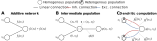
\includegraphics{media/chapters/03_nlif/03_01/nef_multivariate_functions.pdf}%
	{\phantomsubcaption\label{fig:nef_multivariate_functions_a}}%
	{\phantomsubcaption\label{fig:nef_multivariate_functions_b}}%
	{\phantomsubcaption\label{fig:nef_multivariate_functions_c}}%
	\caption[Using dendritic computation to approximate multivariate functions in the NEF]{Using dendritic computation to approximate multivariate functions in the \NEF. \textbf{(A)} Standard \NEF networks are additive: summation in activity space corresponds to addition in representation space.
	\textbf{(B)} Computing nonlinear multivariate functions $f$ generally requires all variables to be represented in an intermediate population.
	\textbf{(C)} The dendritic computation scheme discussed in here.
	Two pre-populations project onto a post-population with separate excitatory and inhibitory input channels.
	%The nonlinear interaction between these channels is exploited to compute $\phi$.
	}
	\label{fig:nef_multivariate_functions}
\end{figure}

Dendritic computation as pursued here is best explained by reviewing fundamental properties of neural networks, and exploring how mul\-ti\-va\-ri\-ate functions such as $f(x_1, \ldots, x_\ell)$ can be approximated in the \NEF.
Specifically, we compare three different network architectures (cf.~\Cref{fig:nef_multivariate_functions}).
\emph{Additive networks} represent $x_1$, $\ldots$, $x_\ell$ in independent neuron populations.
These networks cannot approximate most multivariate functions.
In contrast, \emph{two-layer networks} represent all variables in a common intermediate population.
These networks are universal approximators.
Lastly, our notion of \emph{dendritic computation} relies on non-linear interaction between independent neural input channels.
While not as powerful as multi-layer networks, dendritic computation can approximate a larger class of functions as additive networks.

\subsection{Additive Multivariate Networks}
\label{sec:additive_net}

As stated above, our goal is to compute multivariate functions $f(x_1, \ldots, x_\ell)$ within the context of the \NEF.
%For the sake of simplicity, we mostly discuss bivariate functions of the form $\phi(x_1, x_2)$, but the same considerations apply to more than two input variables as well.
For the sake of simplicity, assume that two pre-populations representing variables $x_1$, $x_2$, respectively, are connected to a common post-population.
To compute $f(x_1, x_2)$, we must find connection weights $\vec w_{1, i}$, $\vec w_{2, i}$ such that the following holds for every post-neuron $i$
\begin{align}
	a_i(f(x_1, x_2))
		= G_i \bigl[
			\langle \vec e_i, f(x_1, x_2) \rangle
		\bigr]
		\supposedEq G_i\bigl[
			\langle \vec w_{1, i}, \vec a^\mathrm{pre}_1(x_1) \rangle + \langle \vec w_{2, i}, \vec a^\mathrm{pre}_2(x_2)
		\rangle\bigr] \,.
	\label{eqn:nef_multivariate_addition}
\end{align}
Here, $a_i$ is the desired post-neuron activity according to the normative tuning-curve constraint (eq.~\ref{eqn:encoding}).
As discussed in the context of the \NEF transformation principle (cf.~\Cref{sec:nef_transformation}), we assume that the current-translation function $J_i$ is part of the individual neuron response curve $G_i$, and that the currents induced by the pre-populations are summed.

This optimisation problem can be easily solved for multivariate functions that can be decomposed into a sum of two univariate functions, i.e., $f(x_1, x_2) = f_1(x_1) + f_2(x_2)$ (cf.~\Cref{fig:nef_multivariate_functions_a}).
Specifically, we can find weights $\vec w_{1, i}$, $\vec w_{2, i}$ that approximate $f$ using the encoder-decoder split of the \NEF. % \citep[cf.][Section~6.1.2]{eliasmith2003neural}.
Computing decoders $\mat D^{f_1}$, $\mat D^{f_2}$ and applying $(\vec w_i)^T = \vec e_i \mat D$, we have
\begin{align*}
	G_i\bigl[
	  \langle
	  	\vec e_i \mat D^{f_1},
	  	\vec a^\mathrm{pre}_1(x_1)
	  \rangle
	+ \langle
	  	\vec e_i \mat D^{f_2},
		\vec a^\mathrm{pre}_2(x_2)
	\rangle\bigr] = 
	G_i\bigl[\langle \vec e_i, \mat D^{f_1} \vec a_1^\mathrm{pre}(x_1) + \mat D^{f_2} \vec a_2^\mathrm{pre}(x_2) \rangle\bigr]
	\approx a_i\bigl(f_1(x_1) + f_2(x_2)\bigr) \,.
\end{align*}
This equation expresses that addition in activity space (i.e., summing weighted pre-activities, eq.~\ref{eqn:nef_multivariate_addition}) is equal to addition in represented space.
In other words, standard \NEF networks are \emph{additive}.
Summing functions incurs no additional decoding error.

\begin{figure}
	\centering
	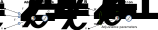
\includegraphics{media/chapters/03_nlif/03_01/perceptron.pdf}%
	{\phantomsubcaption\label{fig:perceptron_a}}%
	{\phantomsubcaption\label{fig:perceptron_b}}%
	\caption[Additive networks are a generalisation of the perceptron]{Additive networks are a generalisation of the perceptron. \textbf{(A)} An additive network is a sum of arbitrary univariate functions. \textbf{(B)} A perceptron is an additive network with functions of the form $f_i(x_i) = w_i x_i + \beta \ell^{-1}$. The weights $w_i$ are learned such that the output approximates a desired function.}
\end{figure}

\subsubsection{Additive networks cannot compute most multivariate functions}
The only way to compute general multivariate functions $f(x_1, x_2)$ in additive networks is to \emph{approximate} $f$ as an additive univariate decomposition.
As is expressed by the following proposition (see Appendix~B.3.1 for a proof), it is impossible to compute many continuous multi-variate $f$ in this way.%
\footnote{We limit our propositions to continuous functions for the sake of simplicity.
However, we conjecture that the same results hold for larger classes of functions, for example square Lebesgue integrable functions.}
This is true even if we can decode arbitrary univariate functions $f_1$, $\ldots$, $f_\ell$ over the pre-variables (this is equivalent to having an infinite number of pre-neurons, see below), and we were able to freely choose a fixed nonlinearity $\sigma$ (cf.~\Cref{fig:perceptron_a}).

\begin{restatable}{theorem}{ThmXorGeneral}
\label{thm:xor_general}
Let $\ell > 1$, $\Xrepr \subset \mathbb{R}^\ell$ and $\mathbb{Y} \subset \mathbb{R}$ be compact sets of full dimensionality, and $\sigma$, $f$, $f_i$ be continuous.
For any fixed $\sigma : \mathbb{R} \longrightarrow \mathbb{Y}$, there always exist $f : \Xrepr \longrightarrow \mathbb{Y}$ such that there is no $f_1$, $\ldots$, $f_\ell : \mathbb{R}  \longrightarrow \mathbb{R}$ with
$f(x_1, \ldots, x_\ell) = \sigma\bigl( f_1(x_1) + \ldots + f_\ell(x_\ell) \bigr)$ for all $(x_1, \ldots, x_\ell) \in \Xrepr$.
\end{restatable}

\begin{figure}
	\centering
	\includegraphics{media/chapters/03_nlif/03_01/xor_visualisation.pdf}%
	{\phantomsubcaption\label{fig:xor_visualisation_a}}%
	{\phantomsubcaption\label{fig:xor_visualisation_b}}%
	{\phantomsubcaption\label{fig:xor_visualisation_c}}%
	{\phantomsubcaption\label{fig:xor_visualisation_d}}%
	{\phantomsubcaption\label{fig:xor_visualisation_e}}%
	\caption[Visualisation of the XOR decision problem for different classifiers]{Visualisation of the \XOR decision problem for different classifiers. The goal is to find classifier parameters such that the four samples are classified as depicted.
	The background corresponds to the sign of the monotonic function $\sigma(\xi)$.
	\textbf{(A)} The linear decision boundary formed by the Perceptron cannot solve the \XOR problem.
	\textbf{(B)} This holds for any function of the form $\sigma(f_1(x_1) + f_2(x_2))$, here $f_1(x_1) = \cos(2\pi x_1)$ and $f_2(x_2) = \sin(2\pi x_2)$.
	\textbf{(C)} A multi-layer Perceptron (MLP) of the form $\sum_i w_i \sigma(e_i^1 x_1 + e_i^2 x_2 + \beta_i )$ can solve the problem, although the decision boundary is quite erratic.
	\textbf{(D)} An alternative solution using the nonlinearity $\sigma'(\xi) = \sigma(\xi^2 - 1)$.
	\textbf{(E)} Multiplication of two real-valued variables $x_1$, $x_2$ can be seen as a continuous form of the \XOR problem.
	Additive networks cannot compute this function.
	}
	\label{fig:xor_visualisation}
\end{figure}

\subsubsection{The Perceptron and XOR}
Consider monotonic $\sigma$ and affine $f_i$ of the form $w_i x_i + \beta \ell^{-1}$.
We obtain the \emph{perceptron}, an early single-layer neural network (cf.~\Cref{fig:perceptron_b}; \cite{rosenblatt1958perceptron}).
\Citet[Chapter~2; originally published in 1969]{minsky1987perceptrons} point out that such networks cannot compute the boolean \XOR function (\Cref{fig:xor_visualisation_a}).%
\footnote{\Citet{minsky1987perceptrons} note that the perceptron was proved by Rosenblatt to \enquote{learn to do anything it was possible to program it to do}; this ambiguous statement endowed researchers with a surplus of optimism---especially since perceptrons sometimes learned difficult problems.
Among other factors, realising that these networks could not be \emph{programmed} to solve trivial problems such as \XOR led to \enquote{the first AI winter} \citep[e.g.,][]{muthukrishnan2020brief}.}
%In the continuous domain, the same is true for multiplication over $\mathbb{X} = [-1, 1]^2$, that is $\phi(x_1, x_2) = x_1 x_2$ (\Cref{fig:xor_visualisation_a}).
Even the general additive networks from our theorem cannot solve a \emph{weaker} version of the \XOR problem, formalised below.

\begin{definition}
\label{def:weak_xor}
A function $\phi(x_1, x_2)$ solves the \emph{weak \XOR problem} if there exist $a_0, b_0, a_1, b_1$ with
\begin{align*}
	\big( \phi(a_0, b_0) < \phi(a_0, b_1) \big) \wedge
	\big( \phi(a_1, b_1) < \phi(a_0, b_1) \big) \wedge
	\big( \phi(a_0, b_0) < \phi(a_1, b_0) \big) \wedge
	\big( \phi(a_1, b_1) < \phi(a_1, b_0) \big) \,.
\end{align*}
\end{definition}

%That is, we merely require $\phi(a_0, b_0)$ and $\phi(a_1, b_1)$ to be larger than $\phi(a_0, b_1)$ and $\phi(b_1, b_0)$.

\begin{restatable}{theorem}{ThmWeakXor}
\label{thm:weak_xor}
Let $\sigma$ be monotonic. Then, an additive network of the form $\phi(x_1, x_2) = \sigma(f_1(x_1) + f_2(x_2))$ cannot solve the weak \XOR problem.
\end{restatable}
This may be surprising, given that, as depicted in \Cref{fig:xor_visualisation_b}, we can generate highly nonlinear classification boundaries.
We provide a proof in Appendix~B.3.2.

To solve the \XOR problem, we can either, as discussed next, use multi-layer networks (cf.~\Cref{fig:xor_visualisation_c}), or, alternatively make $\sigma$ non-monotonic.
As depicted in \Cref{fig:xor_visualisation_d}, setting $\sigma(\xi) = \xi^2 - 1$ allows us to solve the \XOR problem.
This illustrates our goal with dendritic computation: exploit \enquote{more powerful} $\sigma$ to approximate a larger class of functions.

Still, the functions that we can compute using additive networks are limited, even if we can freely choose $\sigma$.
For example, we can compute $x_1 x_2$ for $(x_1, x_2) \in [\epsilon, 1]^2$ and $0 < \epsilon < 1$ by setting $f_1$ and $f_2$ to the logarithm and $\sigma$ to the exponential.
However, it is impossible to find functions that compute multiplication over all four quadrants---which can be seen as a continuous version of the \XOR problem (\Cref{fig:xor_visualisation_e}).
More precisely, allowing $x_1$, $x_2$ to be zero makes it impossible to compute multiplication in these networks (proof in Appendix~B.3.3).
\begin{restatable}{theorem}{ThmMultiplication}
\label{thm:multiplication}
There are no continuous, real-valued functions $f_1$, $f_2$, $\sigma$ such that $\sigma(f_1(x_1) + f_2(x_2)) = x_1 x_2$ for all $(x_1, x_2) \in [0, 1]^2$.
\end{restatable}


%Choosing this $\sigma$ implicitly introduces a non-linear interaction between the variables $x_1$, $x_2$, for example
%\begin{align*}
%	\sigma\left( (w_1 x_1 + w_2 x_2 + \beta)^2 - 1\right) = 
%	\sigma\left( w_1^2 x_1^2 + w_2^2 x_2^2 + 2 w_1 w_2 x_1 x_2 + 2 w_1 \beta x_1 + 2 w_2 \beta x_2 + \beta^2  - 1\right) \,.
%\end{align*}
%The product-term $w_1 w_2 x_1 x_2$ can be exploited to %compute multiplication-like functions.
%Still, as stated in Theorem~1, there inevitably is a large set of functions that we cannot compute.
% TODO Add reference

\subsection{Two-Layer Networks and Intermediate Populations}
\label{sec:two_layer_intermediate}

\begin{figure}
	\includegraphics{media/chapters/03_nlif/03_01/mlp.pdf}
	\caption[Sketch of a two-layer neural network]{Sketch of a two-layer neural network with rectified linear units (ReLUs). If the encoding vectors $\vec e_i$ and the biases $\beta_i$ are sampled appropriately, this network is a universal function approximator.}
	\label{fig:mlp}
\end{figure}

As already mentioned in \Cref{sec:nef_transformation}, an individual \NEF population can be interpreted as a two-layer neural network (cf.~\Cref{fig:mlp}).
As long as the encoding vectors are sampled from the $\ell$-dimensional hypersphere and $x$-intercepts are uniformly distributed, such a neuron population is a universal function approximator, that is, we can compute arbitrary functions $f(x_1, \ldots, x_\ell)$ over the variables represented in the population.
The following theorem states this more formally for neurons with a rectified linear unit (\ReLU) nonlinearity, i.e., $\sigma(\xi) = \max\{0, \xi\}$.

\begin{restatable}{theorem}{ThmTwoLayerUniversal}
\label{thm:two_layer_universal}
Let $\ell \geq 1$, and $f : \mathbb{B}^\ell \longrightarrow \mathbb{R}$ be a continuous function mapping from the $\ell$-dimensional unit ball onto $\mathbb{R}$.
Furthermore, let $\sigma(\xi) = \max\{0, \xi\}$, $\vec e_i$ be sampled uniformly from the unit-sphere $\mathbb{S}^\ell$, and $\alpha_i$ and $\beta_i$ be sampled such that $-\beta_i / \alpha_i$ is uniformly distributed between $[-1, 1]$ and $\alpha_i + \beta_i$ is uniform over $(0, 1]$.
There exist $d_i \in \mathbb{R}$ such that
\begin{align}
	\vspace*{-0.5em}
	f(\vec x) = \lim_{\Npop \to \infty} \sum_{i = 1}^{\Npop} d_i \sigma\bigl( \alpha_i \langle \vec e_i, \vec x \rangle + \beta_i \bigr) \quad \text{for all} \quad \vec x \in \mathbb{B}^\ell \,.
	\label{eqn:two_layer_network}
\end{align}
\end{restatable}
\vspace*{-0.5em}\noindent
This follows directly from \citet{hornik1989multilayer}.
We provide a more thorough discussion in \Cref{app:thm_two_layer_universal}.
This theorem can be extended to hold for arbitrary compact domains $\Xrepr$, codomain dimensionalities, and other neural nonlinearities $\sigma$.

%It may not be obvious why \cref{eqn:two_layer_network} describes a \enquote{two-layer} neural network.
%In essence, the encoding weights $\vec e_i$ map $\vec x$ onto the input of one of the $N$ neurons with nonlinearity $\sigma$.
%This step forms the \enquote{first} or \enquote{hidden layer}.
%The decoding weights $d_i$ then map the neural activities $\sigma(\xi_i)$ onto the output, which forms the \enquote{second layer} (cf.~Figure~2.20).
%% TODO: Add actual reference

\subsubsection{The role of uniformly sampled encoders}
Theorem~\ref{thm:two_layer_universal} requires that the encoding vectors $\vec e_i$ are uniformly sampled from the hypersphere $\mathbb{S}^\ell$.%
\footnote{There are weaker requirements for specific $f$.
As demonstrated by \citet{gosmann2015precise} in the context of multiplication, there are certain distributions of encoding vectors that minimise the decoding error.
Global optimisation methods such as stochastic gradient descent systematically select such \enquote{optimal} encoders.}
To see why this is important, consider the case where the $\vec e_i$ are axis-aligned, i.e., $\|\vec e_i\|_0 = 1$ (cf.~Appendix~A.1).
% TODO: Add reference for zero-norm in Appendix~A.1
In this case, we can split \cref{eqn:two_layer_network} into $\ell$ sub-networks, each decoding a function over a single variable $x_\ell$
\begin{align*}
		\sum_{i = 1}^N d_i \sigma\bigl( \langle \vec e_i, \vec x \rangle - \beta_i \bigr)
	= 	\sum_{j = 1}^\ell \sum_{i = 1}^{N_j} d_{j i} \sigma\bigl( e_{j i} x_j - \beta_{j i} \bigr) \,, \text{where } e_{j i} \in \{ -1, 1\} \,.
\end{align*}
This is equivalent to the additive networks we discussed before.
We can only decode sums of univariate functions over the individual $x_j$ from the pre-population.

\subsubsection{Intermediate populations}
As discussed by \citet[Chapter~6]{eliasmith2003neural}, multivariate functions $f(x_1, x_2)$ can in general only be computed in the \NEF if all variables $x_1$, $x_2$ are represented in a common population.
Correspondingly, if all variables are represented in separate univariate populations, we must add an intermediate population to our network that represents a vectorial quantity $\vec z = (x_1, x_2)$ (cf.~\Cref{fig:nef_multivariate_functions_b}).
We can construct such a representation from two univariate populations by computing the functions $f_1(x_1) = (x_1, 0)$ and $f_2(x_2) = (0, x_2)$ in the connections to the intermediate population.
According to Theorem~\ref{thm:two_layer_universal} we can then decode any multivariate function from the intermediate population.

\subsubsection{Potential issues with intermediate populations}
In theory, the number of neurons required to cover a $d$-dimensional space rises exponentially with $d$.
Representing a $d$-dimensional quantity in an intermediate population can thus require a large number of neurons to achieve a certain decoding error for all target functions.
In practice, it is quite difficult to judge the number of neurons required to decode a certain function $f$ a-priori; the decoding error heavily depends on $f$ and the encoding vectors $\vec e_i$.

Another problem arises when modelling neurobiological systems.
There may be no indication that an intermediate population exists in a particular biological circuit, although the hypothesised high-level function is a multivariate function.
An example of this would be the attention system in layer six of the cortex mentioned in the introduction, where a group of control neurons modulates another population without an intermediary \citep{bobier2014unifying}.

Finally, there is the issue of noise.
In spiking neural networks, every intermediate neuron population introduces additional noise due to static distortion and spike noise \citep[Section~2.2.2]{eliasmith2003neural}.
We see the effects of this later.

\subsection{Dendritic Computation}
\label{sec:dendritic_computation_theory_dendritic}

Dendritic computation is one way to partially alleviate the limitations arising from intermediate populations.
The basic idea is that each neuron possesses $k$ \emph{input channels}.
Input fed through these channels interacts nonlinearly, modelling information processing within the dendrites.

\begin{figure}
	\includegraphics{media/chapters/03_nlif/03_01/dendritic_computation.pdf}%
	{\phantomsubcaption\label{fig:dendritic_computation_net}}%
	{\phantomsubcaption\label{fig:dendritic_computation_fun}}%
	\caption[Overview of our notion of dendritic computation.]{Overview of our notion of dendritic computation. \textbf{(A)} Neuron with an excitatory and inhibitory input channel. In a network context, these functions are decoded from pre-populations representing these variables. Connectivity can be constrained such that excitatory and inhibitory pre-neurons only connect to the corresponding channel. \textbf{(B)} Conceptually, each channel receives a sum of univariate functions computed over the pre-variables $x_1$, $\ldots$, $x_\ell$.}
\end{figure}

Mathematically, the response curve describing the average neural activity is now a multivariate function $\mathscr{G}[\xi_1, \ldots, \xi_k]$, where the $\xi_i$ are linear combinations of the pre-activities (\Cref{fig:dendritic_computation_net}).
To compute $f(x_1, \ldots, x_\ell)$, the following must hold for each post-neuron $i$
\begin{align}
	\begin{aligned}
	a_i\bigl(f(x_1, \ldots, x_\ell)\bigr) &\supposedEq
	\mathscr{G} \bigl[
		\langle \vec w_{1, i}^1, \vec a^\mathrm{pre}_1(x_1) \rangle + \ldots +
		\langle \vec w_{\ell, i}^1, \vec a^\mathrm{pre}_\ell(x_\ell) \rangle, \ldots,\\
%	&~\quad\quad\vdots, \\
	&~\hspace{1.86em}
		\langle \vec w_{1, i}^k, \vec a^\mathrm{pre}_1(x_1) \rangle + \ldots +
		\langle \vec w_{\ell, i}^k, \vec a^\mathrm{pre}_\ell(x_\ell) \rangle
	\bigr]
	\end{aligned}
	\label{eqn:dendritic}
\end{align}
where $a_i(f(x_1, \ldots, x_\ell))$ expresses the normative tuning constraint defined in \cref{eqn:encoding}.

Note that we deliberately left the concept of an \enquote{input channel} open.
An input channel could either refer to a different location in the dendritic tree, different synapse types (e.g., excitatory or inhibitory synapses), or even the influence of other signalling molecules.
We discuss a particular neuron model family with multiple input channels in \Cref{sec:nlif}.

\subsubsection{Mathematical analysis}
More formally, using $\sigma(\xi_1, \ldots, \xi_\ell)$ as an abstract nonlinearity and assuming that we can compute any univariate function $g_i^j$ over $\xi_1, \ldots, \xi_\ell$, we have (\Cref{fig:dendritic_computation_fun})
\begin{align}
	\sigma \bigl(
		g_{1}^1(x_1) + \ldots + g_{\ell}^1(x_\ell), \ldots, g_{1}^k(x_1) + \ldots + g_{\ell}^k(x_\ell)
	\bigr) = \phi(x_1, \ldots, x_\ell) \,.
	\label{eqn:dendritic_computation_theory}
\end{align}
It is trivial to show that such networks are more powerful than additive networks.
For example, let $\sigma(\xi_1, \xi_2) = \xi_1 \xi_2$.
Now, setting the functions feeding into the second channel to one, i.e., $g_{1, i}^2(x_1) = \ldots = g_{\ell, 1}^2(x_\ell) = 1$, we obtain an additive network.
Of course, in contrast to additive networks, we can use the same $\sigma$ to compute products of the pre-variables.
Still, dendritic computation computation networks are not universal approximators:
\begin{conjecture}
\label{thm:dendritic_compuation_incomplete}
Let $\ell > 1$, $\Xrepr \subset \mathbb{R}^\ell$ and $\mathbb{Y} \subset \mathbb{R}$ be compact sets of full dimensionality, and $\sigma$, $f$, $g^j_i$ be continuous.
For any fixed $\sigma : \mathbb{R}^k \longrightarrow \mathbb{Y}$, there always exist $f : \Xrepr \longrightarrow \mathbb{Y}$ such that there are no $g^1_1, \ldots, g^1_\ell, \ldots, g^k_1, \ldots, g^k_\ell : \mathbb{R}  \longrightarrow \mathbb{R}$ with the property
\begin{align*}
	f(x_1, \ldots, x_\ell) = \sigma(\xi_1, \ldots, \xi_k) = \sigma\bigl( g^1_1(x_1) + \ldots + g^1_\ell(x_\ell), \ldots,  g^k_1(x_1) + \ldots + g^k_\ell(x_\ell)\bigr) \text{ for all } \vec x \in \Xrepr \,.
\end{align*}
\end{conjecture}
\noindent While a rigorous proof eludes us, counting the degrees of freedom (DOF) required to describe an $\ell$-dimensional function $f$ suggests that this should be true.
Given $\oh$ orthogonal one-dimensional basis functions, the corresponding $\ell$-dimensional basis has $\oh^\ell$ basis functions.
Correspondingly, $\oh^\ell$ DOF are required to describe an $\ell$-dimensional $f$ with a basis of order $\oh$.
However, when using dendritic computation, we only use $k \ell$ one-dimensional functions; correspondingly, there are only $\oh k \ell$ DOF.
For $\oh \to \infty$, and $\ell > 1$, $\oh k \ell$ grows much slower than $\oh^\ell$.
Hence, there are always functions than cannot be computed using dendritic computation.%
\footnote{Mathematically, the cardinality of the set of continuous functions $f$ constructed from a function basis of order $\oh$ is $|\mathbb{R}^{\oh^\ell}|$, while the cardinality of functions that can be constructed using dendritic computation is $|\mathbb{R}^{\oh k \ell}|$.
Unintuitively, even for $\oh \to \infty$, it holds $|\mathbb{R}^{\oh^\ell}| = |\mathbb{R}^{\oh k\ell}| = \mathfrak{c}$, where $\mathfrak{c}$ is the cardinality of the continuum \citep[e.g.,][Chapter~4]{jech2003set}.
Fortunately, this is irrelevant in practice.
Assuming some baseline precision and dynamic range of the generalised Fourier coefficients, there are only finitely many parameters $N$ that can be used to uniquely characterise each function. It clearly holds $N^{\oh^\ell} \gg N^{\oh k \ell}$ for $\ell > 1$ and $\oh \to \infty$.}

\subsection{Numerical Exploration}
\label{sec:dendritic_computation_theory_numerical}

The above discussion offers only limited insight into the practical implications of using dendritic computation.
The goal of this section is to provide a numerical analysis of our different network types.
Specifically, we characterise the \enquote{computational power} of a network by approximating two-dimensional functions $f(x_1, x_2)$ of varying complexity.
More \enquote{powerful} networks should be capable of computing \enquote{more complex} $f(x_1, x_2)$ at lower errors than other networks.
Since the \enquote{complexity} of a function is somewhat ill-defined, we use frequency content as a proxy.
Functions with a higher spatial bandwith contain more information \citep[cf.][]{shannon1949communication} than functions only composed of lower frequencies and should thus qualify as \enquote{more complex}.

\subsubsection{Generating random test functions}

\begin{figure}
	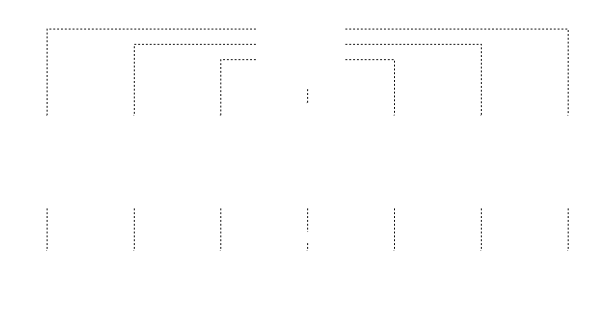
\includegraphics{media/chapters/03_nlif/03_01/2d_functions_overview_overlay.pdf}%
	\kern-157.24mm\includegraphics{media/chapters/03_nlif/03_01/2d_functions_overview.pdf}
	\caption[Overview of our procedure for generating random 2D functions]{Overview of our procedure for generating random 2D functions. \textbf{(A)} We sample a 2D array from a normal distribution (only a portion of the array is depicted; the size $n' \times n'$ depends on the filter width). \textbf{(B)} The noise is filtered by convolving with a Gaussian kernel with standard-deviation $\rho$ (for large filter widths, i.e., small $\rho^{-1}$, only a small portion of the filter is depicted). \textbf{(C)} The resulting functions are transformed to have mean zero (i.e., no DC component) and a standard deviation of one.}
	\label{fig:2d_functions_overview}
\end{figure}

To generate sampled random $f(x_1, x_2)$, we use the scheme depicted in \Cref{fig:2d_functions_overview}.
In a nutshell, we draw $n' \times n'$ points from a normal distribution and apply a 2D Gaussian filter with standard deviation $\rho$.
We then extract the desired $n \times n$ samples not affected by boundary effects, and normalise the result to zero mean and unit standard deviation.
As a result, small $\rho^{-1}$ (i.e., large filters), result in almost linear functions, whereas large $\rho^{-1}$ (small filters) result in high-frequency functions.%
\footnote{
Note that this scheme generates aperiodic functions.
Correspondingly, while the filtered grid of $n' \times n'$ samples is band-limited, the final $n \times n$ samples are not.
High frequencies are required to represent the discontinuous boundary---a result of applying a box-window to our data (cf.~the \enquote{windowing theorem}; e.g.,~\cite{oppenheim2009discretetime}, Section~2.9.7).
Hence, there is no trivial way to sample these functions directly the frequency domain, and to make use of the fast inverse Fourier transformation.
Still, this scheme can be implemented efficiently by separating the Gaussian filters into horizontal and vertical components \citep[e.g.][]{bolon2006twodimensional}.
}

\subsubsection{Network models}
To compare the above networks types, we could construct neural networks and compare approximation errors for our randomly generated two-dimensional functions $f(x_1, x_2)$.
However, as a simplification, we can replace the pre-populations by the first $\oh$ Legendre polynomials $P_i(x)$.%
\footnote{We discuss Legendre polynomials in \Cref{sec:function_bases}. Note that we use a discretised version of the Legendre basis, \enquote{Discrete Legendre Orthogonal Polynomials} \citep[DLOPs;][]{neuman1974discrete,stockel2021discrete}.}
This is possible because the principal components of neural populations resemble Legendre polynomials \citep[Chapter~7]{eliasmith2003neural}.
Furthermore, using a function basis of order $\oh$ connects back to our previous theoretical discussion of dendritic computation in terms of degrees of freedom.
The number of basis functions that can be decoded well from a pre-population depends on the number of neurons in that population.
We explore this in more detail below.
%In a sense, thus we replace random neuron populations with the corresponding \enquote{optimal} orthogonal basis.

Replacing the pre-population in the additive network with $\oh$ basis functions, and under the assumption that $\sigma(\xi) = \xi$ (there is no additional nonlinearity), we get
\begin{align}
	f_\mathrm{add}(x_1, x_2) &= g_1(x_1) + g_2(x_2) = \sum\nolimits_{i = 0}^{\oh} w^1_{i} P_i(x_1) + \sum\nolimits_{i = 0}^{\oh} w^2_{i} P_i(x_2) \,,
	\label{eqn:f_add}
\end{align}
where $w_i^1$, $w_i^2$ (for $2o$ degrees-of-freedom; DOF) can be computed using least squares.
For our analysis of dendritic computation, we choose $\sigma(\xi_1, \xi_2) = \xi_1 \xi_2$ as a nonlinearity $\sigma$ and obtain
\begin{align}
	\begin{aligned}
		f_\mathrm{den}(x_1, x_2)
			&= \sigma\big(g^1_1(x_1) + g^1_2(x_2), g^2_1(x_1) + g^2_2(x_2)\big) \\
			&= \left( \sum\nolimits_{i = 0}^{\oh} w^1_{i} P_i(x_1) + \sum\nolimits_{i = 0}^{\oh} w^2_{i} P_i(x_2) \right)
			   \left( \sum\nolimits_{i = 0}^{\oh} w^3_{i} P_i(x_1) + \sum\nolimits_{i = 0}^{\oh} w^4_{i} P_i(x_2) \right)  \,.
	\end{aligned}
	\label{eqn:f_den}
\end{align}
Solving for $w^1_{i}$, $w^2_{i}$, $w^3_{i}$, $w^4_{i}$ (for a total of $4\oh$ DOF) is a non-convex optimisation problem that tends to possess numerous local minima.
We use the BFGS quasi-Newton method \citep[Chapter~8]{nocedal2006numerical} with ten random initialisations and pick the best solution.

Finally, we emulate the universal approximator nature of multi-layer networks by constructing an additive network based on two-dimensional basis functions $P_{ij}(x_1, x_2) = P_{i}(x_1) P_j(x_2)$:
\begin{align}
	f_\mathrm{mlp}(x_1, x_2)
		&= \sum\nolimits_{i = 0}^{\oh} \sum\nolimits_{j = 0}^{\oh} w_{ij} P_{ij}(x_1, x_2) = \sum\nolimits_{i = 0}^{\oh} \sum\nolimits_{j = 0}^{\oh} w_{ij} P_{i}(x_1) P_j(x_2) \,.
	\label{eqn:f_mlp}
\end{align}
Again, the weights $w_{ij}$ (for a total of $o^2$ DOF) can be optimally determined using least-squares.

%We can immediately see that $f_\mathrm{add}$ does not contain products between $x_1$ and $x_2$.
Note that if we had chosen $\sigma(\xi) = \xi^2$ in \Cref{eqn:f_add}, then $f_\mathrm{add}$, $f_\mathrm{den}$ and $f_\mathrm{mlp}$ would all be composed of the same $\oh^2$ product-terms.
Hence, the difference between these networks ultimatley lies in the degrees of freedom; additive networks and dendritic computation are fundamentally constrained in how these product-terms can be combined.
In particular, we can expect $f_\mathrm{den}$ to compare favourably well to $f_\mathrm{mlp}$ if $4\oh \leq \oh^2$, that is $\oh \leq 4$.
This is the case if only the first few basis functions can be decoded well from the pre-population.

\subsubsection{Experiment: Decoding random functions}

\begin{figure}
	\includegraphics{media/chapters/03_nlif/03_01/dendritic_computation_legendre_overview.pdf}%
	{\phantomsubcaption\label{fig:dendritic_computation_legendre_overview_a}}%
	{\phantomsubcaption\label{fig:dendritic_computation_legendre_overview_b}}%
	{\phantomsubcaption\label{fig:dendritic_computation_legendre_overview_c}}%
	{\phantomsubcaption\label{fig:dendritic_computation_legendre_overview_d}}%
	{\phantomsubcaption\label{fig:dendritic_computation_legendre_overview_e}}%
	\caption[Function approximation using different network setups]{Function approximation using different network setups.
	\textbf{(A)} Grid of the first $10 \times 7$ 2D Legendre basis functions $\tilde P_{ij}(x_1, x_2)$. The 1D basis functions depending only on $x_1$ and $x_2$ are to the left/top of the dashed lines.
	\textbf{(B)} Randomly generated target functions of different complexity $\rho^{-1}$.
	\textbf{(C,~D,~E)}~Approximations of the target functions using the different networks discussed in the text. Inset error values are the normalised RMSE in percent.
	}
	\label{fig:dendritic_computation_legendre_overview}
\end{figure}

\begin{figure}
	\includegraphics{media/chapters/03_nlif/03_01/dendritic_computation_fourier_example.pdf}%
	{\phantomsubcaption\label{fig:dendritic_computation_fourier_example_a}}%
	{\phantomsubcaption\label{fig:dendritic_computation_fourier_example_b}}%
	{\phantomsubcaption\label{fig:dendritic_computation_fourier_example_c}}%
	\caption[Computing functions with different spatial frequencies using different network types]{
	Computing functions with different spatial frequencies using different network types.
	Each line is the median \NRMSE when approximating with respect to the \RMS of the target function over $N = 1000$ randomly generated functions with spatial filter coefficient $\rho^{-1}$ using $d$ Legendre basis functions (cf.~\Cref{fig:2d_functions_overview}).
	Shaded areas correspond to the 25/75-percentile.
	\textbf{(A, B)}
	Median error for different filter coefficients $\rho^{-1}$ for fixed basis function counts~$d$. Dashed lines correspond from the median from the neighbouring diagram. Vertical dotted line is at $\rho^{-1} = 2$.
	\textbf{(C)}
	Median error over different basis function counts for a fixed filter coefficient $\rho^{-1} = 2$.
	Increasing the basis function count only substantially decreases the error in the case of an additive network with 2D bases.
	}
	\label{fig:dendritic_computation_fourier_example}
\end{figure}

We compare the three network types by varying the spatial low-pass filter size $\rho^{-1}$ and the basis order $\oh$.
\Cref{fig:dendritic_computation_legendre_overview} provides an overview of the overall procedure.
The one- and two-dimensional Legendre polynomials are depicted in \Cref{fig:dendritic_computation_legendre_overview_a}, randomly generated target functions are depicted in \Cref{fig:dendritic_computation_legendre_overview_b}.
These functions are reconstructed using the function approximators defined above (\Cref{fig:dendritic_computation_legendre_overview_c,fig:dendritic_computation_legendre_overview_d,fig:dendritic_computation_legendre_overview_e}).

As expected, the network type has a large influence on the reconstruction error.
While the additive network $f_\mathrm{add}$ only fares well for almost linear functions, $f_\mathrm{mlp}$ reaches reasonable approximation errors even for complex target functions.
The dendritic network $f_\mathrm{den}$ sits somewhere in between;
$f_\mathrm{den}$ can be used to decode the target function for $\rho^{-1} = 1$ at a reasonable $6\%$ \NRMSE, while failing to reconstruct the target function for $\rho^{-1} = 3.16$ at a $44\%$ error.

\Cref{fig:dendritic_computation_fourier_example} depicts the results of a more systematic experiment.
For a fixed basis function count (\Cref{fig:dendritic_computation_fourier_example_a}), the error achieved with an additive network $f_\mathrm{add}$ increases almost with $\rho$ on a log-log plot, while both $f_\mathrm{den}$ and $f_\mathrm{mpl}$ possess a sublinear plateau.

Increasing the basis order $\oh$ (\Cref{fig:dendritic_computation_fourier_example_b}) has only a small effect on $f_\mathrm{add}$ and $f_\mathrm{den}$.
We only observe a small decrease in error for $f_\mathrm{den}$ below $\rho^{-1} < 0.5$, whereas there is virtually no change in error for $f_\mathrm{add}$.
Conversely, in the context of $f_\mathrm{mlp}$, the entire error curve is shifted to the right when increasing $o$.
In other words, increasing the basis function order $o$ truly allows $f_\mathrm{mlp}$ to compute more complex functions, whereas $f_\mathrm{add}$ and $f_\mathrm{den}$ are fundamentally limited in the maximum complexity of the functions that can be computed in this manner.

This is even more clearly visible in \Cref{fig:dendritic_computation_fourier_example_c}, where we keep the spatial filter coefficient $\rho^{-1}$ fixed, and sweep over the basis order $o$ instead.
Increasing $\oh$ consistently decreases the error for $f_\mathrm{mlp}$ down to the base-line error induced by regularisation, while the errors for $f_\mathrm{add}$ and $f_\mathrm{den}$ plateau much sooner.
Interestingly, the point at which $f_\mathrm{den}$ and $f_\mathrm{mlp}$ diverge is at $\oh = 4$, which is exactly as we predicted above.


\subsubsection{Experiment: Determining the number of decodable basis functions $d$}

\begin{figure}
	\centering
	\includegraphics{media/chapters/03_nlif/03_01/decode_basis_functions.pdf}
	\caption[Number of decodable basis functions over the number of neurons]{Number of decodable basis functions over the number of neurons. Each line is the mean number of Legendre polynomials  that can be decoded with an error smaller than the indicated threshold from a ReLU neuron population of size $n$ (mean is over $100$ trials). The three columns correspond to a one-, two- and three-dimensional population. The total number of basis functions tested for each data point is $20^\ell$, where $\ell$ is the dimensionality of the population.
	The number of decodable basis functions is not drastically larger for higher-dimensional neuron populations.}
	\label{fig:decode_basis_functions}
\end{figure}

An intrinsic assumption of the above experiment (particularly in $f_\mathrm{mlp}$, eq.~\ref{eqn:f_mlp}) is that the number of decodable basis functions $d$ is given as $d = \oh^\ell$, where $\oh$ is the order of the underlying basis, and $\ell$ is the number of dimensions represented by the pre-population.
However, in practice, this is almost never the case---increasing the dimensionality of a neuron population only has a small impact on the absolute number of decodable basis functions.

This is depicted in \Cref{fig:decode_basis_functions}, where we vary the number of neurons in the pre-population and count the number of $\ell$-dimensional Legendre basis functions that can be decoded with an \NRMSE below some threshold.
Given a $3.2\%$ error threshold and $1000$ neurons, we are able to decode $d = 5$ orthogonal basis functions from the one-dimensional population, $d = 6$ from the two- and $d = 10$ functions three-dimensional population.
While this is a substantial increase in the number of decodable functions, it is nowhere near the exponential increase that we would expect from increasing the order of the underlying basis.

This suggests that, in some scenarios, dendritic computation schemes could outperform multi-layer networks.
Let $d$ and $d'$ be the number of basis functions that can be decoded from a one- and $\ell$-dimensional population, respectively.
Dendritic computation has more \DOF if $k \ell d > d'$, and could thus approximate a larger class of functions below some error threshold.

This analysis should be taken with a grain of salt, since we do not take redundant \DOF into account and rely on a questionable binary notion of a basis function being \enquote{decodable}.
Still, as we will see in \Cref{sec:two_comp_lif,sec:nlif_opt}, dendritic computation can indeed outperform multi-layer networks in practice.

\subsubsection{Conclusion}
Our numerical experiments confirm that, under optimal circumstances, dendritic computation schemes can only compute some functions better than purely additive networks.
This is independent of the order of the function basis induced by the pre-populations.
Our analysis also suggests that dendritic computation may be a viable alternative if only few multivariate basis functions can be decoded well from an intermediate population.

%
%\clearpage
%\setcounter{section}{1}
%% !TeX spellcheck = en_GB

\section{Extending the Neural Engineering Framework}
\label{sec:nef_extension}

Up to this point, we have formally defined dendritic computation and discussed its theoretical benefits.
The goal of this section is to open avenues toward systematically integrating multi-compartment neuron models with dendritic trees into \NEF networks using the formalisms discussed above.

Na\"ively, incorporating neurons with multiple nonlinear input channels into the \NEF is merely a matter of solving for $\vec w$ such that \Cref{eqn:dendritic} holds.
Phrasing this as an optimization problem, we must minimise the difference between the desired average activity according to the normative tuning-curve constraint $a_i(\vec x)$ and the average activity according to our multi-variate response curve $\mathscr{G}$.
Using a least-squares loss (and omitting the regularisation term), we have
\begin{align}
	\begin{aligned}
	E &=
	\frac{1}{\vol(\Xrepr)} \int_{\Xrepr} \Bigl( a_i\bigl(\phi(x_1, \ldots, x_\ell)\bigr) -
	\mathscr{G} \bigl[
		\langle \vec w_{1, i}^1, \vec a^\mathrm{pre}_1(x_1) \rangle + \ldots +
		\langle \vec w_{\ell, i}^1, \vec a^\mathrm{pre}_\ell(x_\ell) \rangle, \ldots,\\
	&~\hspace{13.825em}
		\langle \vec w_{1, i}^k, \vec a^\mathrm{pre}_1(x_1) \rangle + \ldots +
		\langle \vec w_{\ell, i}^k, \vec a^\mathrm{pre}_\ell(x_\ell) \rangle
	\bigr] \Bigr)^2 \,dx_1 \ldots dx_\ell \,.
	\end{aligned}
	\label{eqn:dendritic_computation_optimisation}
\end{align}
One way to minimise this loss-function would be to use stochastic gradient descent.
In fact, this can be a viable strategy---and may be the only option for many detailed neuron models.

Still, we would like to suggest a more systematic approach that, in some cases, reduces the task of finding weights to a convex \qprog.
This is more in line with the \enquote{standard} \NEF, where connection weights are computed by solving a convex least-squares problem.

To arrive at a point where we can integrate complex neuron models more seamlessly, we first need to address two of the limitations of the \NEF discussed in \Cref{sec:nef_limitations}.
Specifically, we discuss how to eliminate the bias currents and to account for Dale's principle.
Furthermore, we present a modified version of \Cref{eqn:dendritic_computation_optimisation} that splits the multivarite response curve $\mathscr{G}$ into a multivariate input-dependent nonlinearity $H$ and a univariate response curve $G$.
We avoid decoding subthreshold currents using a technique we call \enquote{subthreshold relaxation}.

\subsection{Decoding the Current-Translation Function}
\label{sec:nef_decode_current}

So far we assumed that the current translation function $J_i(\xi)$ is an intrinsic part of the neuron model.
Our typical choice of $J_i(\xi) = \alpha_i \xi + \beta_i$ introduces a bias current $\beta_i$ into each neuron.
As we elaborated in \Cref{sec:nef_limitations}, this is slightly implausible from a biological perspective.

\Citet{tripp2007neural} demonstrate that it is possible to robustly solve for synaptic weights that approximate arbitrary post-synaptic current functions.
We use this insight to directly approximate the target current $J_i(\langle \vec e_i, \vec x \rangle)$; as a side effect, we implicitly solve for the bias.
Again, assuming that the post-synaptic current is linear in the pre-population activities, we must find a weight vector $\vec w_i$ such that the following regularised loss is minimised
\begin{align}
E = \frac{1}{\vol(\Xrepr)} \int_{\Xrepr} \left( J_i\bigl(\langle \vec e_i, \phi(\vec x)\rangle\bigr) - \langle \vec w_i, \vec a^\mathrm{pre}(\vec x) \rangle \right)^2 \, d\vec x + \lambda \| \vec w_i \|_\mathrm{2}^2\,.
\label{eqn:decode_current}
\end{align}
As before, this equation can be discretised, brought into canonical least squares form, and solved using the regularised Moore-Penrose pseudo inverse (cf.~eqn.~2.22 and 2.23):
\begin{align*}
	\mat W &= \mat A^+ \mat J \,, & \text{where} \quad \mat A^+ &= (\mat A^T \mat A + \lambda N \mat I)^{-1} \mat A^T \,.
\end{align*}
Here, $N$ is the number of samples, $\mat W \in \mathbb{R}^{m \times \Npop}$ is the connection weight matrix, $\mat J \in \mathbb{R}^{N \times m}$ is a matrix of target currents, and $\mat A \in \mathbb{R}^{N \times n}$ is the matrix of pre-activities.

\begin{figure}
	\includegraphics{media/chapters/03_nlif/03_02/current_translation_decoding.pdf}%
	{\phantomsubcaption\label{fig:current_translation_decoding_a}}%
	{\phantomsubcaption\label{fig:current_translation_decoding_b}}%
	{\phantomsubcaption\label{fig:current_translation_decoding_c}}%
	{\phantomsubcaption\label{fig:current_translation_decoding_d}}%
	\caption[Decoding for currents instead of represented values]{Decoding for currents instead of represented values. \textbf{(A)} Tuning curves of a pre-population with $100$ \LIF neurons (only $50$ tuning curves are shown). \textbf{(B)} Decoding affine current translation functions $J_i$ (dotted lines are the target). The function $\phi$ being computed in re\-pre\-sen\-tat\-ion space is the identity function. Dashed line corresponds to the threshold current $J_\mathrm{th} = \SI{1}{\nano\ampere}$.
	\textbf{(C)} Same as \emph{(B)} but for Gaussian current-translation functions $J_i$. Such functions can be used to produce localised tuning curves.
	\textbf{(D)} First six singular values of the two weight matrices $\mat W$ from \emph{(B, C)}.
	Singular values are normalised by dividing by their sum, resulting in the relative contribution of each singular value to the decoding.
	For affine $J_i$, $\mat W$ is of rank $d + 1$ (here $d = 1$);
	Gaussian $J_i$ result in full-rank $\mat W$.
	}
\end{figure}

Importantly, we no longer solve for weights directly in the domain of represented values $\vec x$; this is in contrast to solving for decoders $\mat D$ according to \cref{eqn:lstsq_loss}.
Similarly, we do not solve for target activities $a_i$, as was suggested by our na\"ive loss function in \cref{eqn:dendritic_computation_optimisation}.
Side-stepping the neural nonlinearity $G$ enables a simple least-squares solution.
Furthermore, this optimisation scheme supports arbitrary current-translation functions $J_i$, providing modellers with a greater flexibility over the tuning curve constraint (cf.~\Cref{fig:current_translation_decoding_a,fig:current_translation_decoding_b,fig:current_translation_decoding_c}).

\subsubsection{Low-rank factorisation of $\mat W$}
Solving the optimisation problem in \cref{eqn:decode_current} directly results in weight matrix $\mat W$ instead the low-rank factorisation $\mat W = \mat E \mat D^\phi$.
As discussed in \Cref{sec:nef_transformation}, this factorisation is useful, as it enables $\mat W \vec a$ to be computed in $\mathcal{O}(n)$ instead of $\mathcal{O}(n^2)$.

Fortunately, at least in the case of the affine current-translation function $\alpha_i \langle \vec e_i, \phi(\vec x) \rangle + \beta_i$, we still obtain a factorisable matrix (cf.~\Cref{fig:current_translation_decoding_d}).
The resulting $\mat W$ is merely of rank $d + 1$, where $d$ is the dimensionality of the post-population.
Specifically, the weight matrix can be expressed as a sum of the low-rank factorisation $\mat E \mat D^\phi$ and the outer product of the biases $\vec \beta \in \mathbb{R}^{m \times 1}$ with a decoding vector $\mat D^1 \in \mathbb{R}^{1 \times n}$.
This \enquote{bias-decoder} decodes the constant \enquote{one} from the pre-population.
In other words, it simply holds $\mat W = \mat E \mat D^\phi + \vec \beta \mat D^1$ (cf.~\cite[Chapter~4]{stockel2017point,duggins2017incorporating}).

\begin{figure}
	\includegraphics{media/chapters/03_nlif/03_02/bias_decoding_impact.pdf}%
	{\phantomsubcaption\label{fig:bias_decoding_impact_a}}%
	{\phantomsubcaption\label{fig:bias_decoding_impact_b}}%
	{\phantomsubcaption\label{fig:bias_decoding_impact_c}}%
	{\phantomsubcaption\label{fig:bias_decoding_impact_d}}%
	\caption[Bias decoding and post-population tuning curve accuracy]{Bias decoding and post-population tuning curve accuracy. \textbf{(A)} Pre-population tuning-curves for $n = 50$ \LIF neurons.
	\textbf{(B)}~Error for decoding the identity function compared to decoding a constant (regularisation factor $\sigma = 10$). The error for decoding a constant is minimally larger than that for decoding the identity function.
	\textbf{(C)}~The first four principal components of the tuning curves (for $n = 1000$).
	The principal components resemble the Legendre polynomials, an orthogonal function basis (dotted lines).
	\textbf{(D)} \RMSE between the desired post-population tuning and the actually achieved tuning. Decoding the bias approximately doubles the error compared to intrinsic bias currents.}
\end{figure}

\subsubsection{Impact of decoding bias currents on network function}
%It is difficult to make blanket statements about the impact of bias decoding on the network function.
Generally speaking, decoding biases increases the error between the actual and desired post-population tuning.
The magnitude of this error depends on the pre- and post-population. 
The former determine how well a constant offset can be decoded, the latter determine the magnitude of the required bias currents.

In the case of \enquote{standard} \NEF tuning with uniform $x$-intercepts and random encoders (cf.~\Cref{fig:bias_decoding_impact_a}), constant functions can, counter-intuitively, only be decoded with a slightly higher error than the identity function (error is about $15\%$ higher; cf.~\Cref{fig:bias_decoding_impact_b}).
This becomes apparent when considering the principal components of the pre-population tuning curves.
As, for example, discussed in \citet[Chapter~7]{eliasmith2003neural}, the principal component analysis (PCA) can be seen as \enquote{uncovering} the best orthogonal basis that linearly generates the tuning-curves.
%(see \cite[Chapter~12]{bishop2006pattern} for general information on the PCA).
In turn, the first principal components characterise the functions that can be decoded well from a population.
As illustrated in \Cref{fig:bias_decoding_impact_c}, the principal components $f_i$ of the \enquote{standard} \NEF tuning curves resemble the Legendre polynomials (cf.~\Cref{sec:function_bases} for a definition).
While the second principal component $f_2$ is linear, just like the corresponding Legendre polynomial, $f_1$ differs significantly from the constant first Legendre polynomial.
Decoding constants is hence \enquote{more difficult} than decoding the identity function.

In our example, and as depicted in \Cref{fig:bias_decoding_impact_d}, decoding $J_i$ doubles the \RMSE between the desired and actual post-population tuning.
%This can be countered by doubling the number of pre-neurons.
However, as we will see in the next subsection, there are circumstances where the absence of an intrinsic bias is improves the network performance.

\subsubsection{Accounting for multiple pre-populations}
As we discussed in \Cref{sec:additive_net}, a welcome side effect of intrinsic current-translation is that standard \NEF networks are additive.
Summing the activities $\vec a^\mathrm{pre}_1$, $\ldots$, $\vec a^\mathrm{pre}_\ell$ from multiple pre-populations is equivalent to summing the decoded $f_1(\vec x_1)$, $\ldots$, $f_\ell(\vec x_\ell)$.
This is no longer the case when
%solving for weights $\vec w_i$
minimising the current-based loss in \cref{eqn:decode_current}.

\begin{figure}
	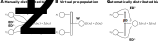
\includegraphics{media/chapters/03_nlif/03_02/nef_decode_bias.pdf}%
	{\phantomsubcaption\label{fig:nef_decode_bias_a}}%
	{\phantomsubcaption\label{fig:nef_decode_bias_b}}%
	{\phantomsubcaption\label{fig:nef_decode_bias_c}}%
	\caption[Accounting for multiple pre-populations when decoding the current-translation function]{Accounting for multiple pre-populations when decoding the current-translation function. \textbf{(A)} Biases can be manually distributed between pre-populations by scaling the bias decoders $\mat D^1_1$ and $\mat D^1_2$ by $\alpha$ and $(1 - \alpha)$, respectively. \textbf{(B)} The general solution is to solve for weights $\mat W$ assuming stacked pre-population activities. The two pre-populations form a \enquote{virtual} pre-population. \textbf{(C)} A combination of the two approaches, where only the bias $\mat D^1$ is decoded from the pre-populations in this way.}
\end{figure}

In the case of the affine $J_i$, each of the $\ell$ connections decodes the bias current, effectively multiplying the bias by $\ell$.
Of course, we can only decode a fraction of the bias from each pre-population (\Cref{fig:nef_decode_bias_a}).
Alternatively, we can combine the pre-populations into a \enquote{virtual pre-population} and let the optimisation process take care of distributing the responsibility for providing the bias between all pre-neurons (\Cref{fig:nef_decode_bias_b}).

More precisely, we explicitly solve for weights that result in $f_1(\vec x_1) + \ldots + f_\ell(\vec x_\ell)$ to be represented in the post-population.
For two populations, and skipping regularisation, we have
\begin{align}
	E =
	\frac{1}{\vol(\Xrepr)^2} \! \iint_{\Xrepr}
	\left(
		J_i\bigl(\langle \vec e_i, f_1(\vec x_1) + f_2(\vec x_2) \rangle\bigr)
		- \langle \vec w_{1, i}, \vec a_1^\mathrm{pre}(\vec x_1) \rangle
		- \langle \vec w_{i, 2}, \vec a_2^\mathrm{pre}(\vec x_2) \rangle
	\right)^2 \, d\vec x_1 d\vec x_2 \,.
	\label{eqn:decode_current_additive}
\end{align}
We can bring this problem into a canonical form by the stacking the pre-activities and weights (see below for an example).
However, note that we now need to sample a much higher-dimensional space.
This is worrisome if we attempt to decode $f_i$ that must be finely sampled to obtain a good decoding.
Again, under the assumption that $J_i$ is affine, it is possible to expand the above integral and to solve for a---relatively easy to decode---population-spanning bias decoder $\mat D^1$ independent of the (untouched) function decoders $\mat D^{f_1}$ and $\mat D^{f_2}$ (\Cref{fig:nef_decode_bias_c}).

%\begin{align*}
%E^\beta &= \frac{1}{\vol(\Xrepr)^2} \! \int_{\Xrepr} \! \int_{\Xrepr} \left( \beta_i - \langle \vec w^\beta_{1, i}, \vec a_1^\mathrm{pre}(\vec x_1) \rangle - \langle \vec w^\beta_{i, 2}, \vec a_2^\mathrm{pre}(\vec x_2) \rangle \right)^2 \, d\vec x_1 \, d\vec x_2
%\end{align*}

\subsection{Nonnegative Weights and Dale's Principle}
\label{sec:nef_nonneg}

Biological neurons tend to follow Dale's principle---they act either excitatorily or inhibitorily (see~\Cref{sec:synaptic_transmission} for more detail).
As discussed in \Cref{sec:nef_limitations}, we ignored this in our weight-solving procedures.
Least-squares assigns arbitrary algebraic signs to the individual weights, typically with an even split between positive and negative (cf.~\Cref{fig:sparsity_and_dales_principle}).
Such weights are not compatible with conductance-based synapses or, more generally, multi-compartment neurons.
Here, modellers connect pre-neurons to specific post-neuron channels.
The corresponding connection weights describe nonnegative quantities, such as the number of vesicles released from the pre-synapse, or the channel density in the post-synapse \citep{roth2009modeling}.

\subsubsection{Solving for weights using non-negative least squares}
Solving for individual synaptic weights in current space suggests a simple procedure to account for nonnegativity.
Assume that each population is arbitrarily split into a group of excitatory and inhibitory neurons.
The somatic input current of post-neuron $i$ in response to pre-synaptic activity is $\langle \vec w_i^+, \vec a^+(\vec x) \rangle - \langle \vec w_i^-, \vec a^-(\vec x) \rangle$;
here, $\vec w_i^+$, $\vec w_i^-$ are nonnegative excitatory and inhibitory weight vectors and $\vec a^+(\vec x)$, $\vec a^-(\vec x)$ are the activities of the excitatory and inhibitory neurons in the pre-population.
Combining this current term with \cref{eqn:decode_current} yields the following optimisation problem for each post-neuron $i$
\begin{align}
	\begin{aligned}
	& \min_{{\vec w}_i^+, {\vec w}_i^-}
	\frac{1}{\vol(\Xrepr)} \int_{\Xrepr} \!
	\left(
		J_i\bigl(\langle \vec e_i, \phi(\vec x) \rangle\bigr)
		- \langle \vec w_{i}^+, \vec a^+(\vec x) \rangle
		+ \langle \vec w_{i}^-, \vec a^-(\vec x) \rangle
	\right)^2 \, d\vec x + \sigma^2 \|\vec w_{i}^+\|_2^2 + \sigma^2 \|\vec w_{i}^-\|_2^2 \\
	& \text{subject to } \vec w_i^+, \vec w_i^- \geq 0 \,.
	\end{aligned}
	\label{eqn:decode_nonneg}
\end{align}
To obtain a canonical least-squares form, let $N$ be the number of samples, $n^+$, $n^-$ be the number of excitatory and inhibitory pre-neurons,%
\footnote{
It does not necessarily hold that $n = n^+ + n^-$; neurons can \emph{technically} be marked as both excitatory and inhibitory. Specifically, the special case $n = n^+ = n^-$ reduces the \NNLS problem to standard least squares.
}
and $\mat A$ be the sampled, stacked, and signed pre-activities $(\mat A^+, -\mat A^-) \in \mathbb{R}^{N \times (n^+ + n^-)}$.
Additionally, let $\mat W$ be the stacked weight matrices $(\mat W^+, \mat W^-) \in \mathbb{R}^{m \times (n^+ + n^-)}$, and $\vec J \in \mathbb{R}^{N \times m}$ be a matrix of sampled target currents. We have
\begin{align}
	\bigl\| \bigl( \mat A^T \mat A + N \sigma^2 \mat I \bigr) \mat W - \mat A^T \mat J \bigr\|_2^2 \quad\quad \text{subject to } \mat W \geq 0 \,.
	\label{eqn:decode_nonneg_canon}
\end{align}
This is a standard nonnegative least-squares (\NNLS) problem that can be solved in polynomial time \citep[Chapter~23]{lawson1995solving}.
An overview of efficient algorithms to solve this kind of problem is given in \citet{chen2009nonnegativity}.%
\footnote{Most linear algebra software packages bundle a solver for nonnegative least-squares; for example \texttt{scipy.optimize.nnls} in SciPy or \texttt{lsqnonneg} in Matlab. Alternatively, a general quadratic programming (\QP) solver can be used; this is what we do in our library \emph{libnlif} that we discuss in \Cref{app:libnlif}.}
Of course, similarly to \cref{eqn:decode_current_additive}, the optimisation problem can be extended to take multiple pre-populations into account.

\begin{figure}[p]
	\centering
	
\includegraphics{media/chapters/03_nlif/03_02/nonnegative_experiments_setup.pdf}\\[0.75cm]	\includegraphics{media/chapters/03_nlif/03_02/nonnegative_experiments.pdf}\\[0.75cm]
	\includegraphics{media/chapters/03_nlif/03_02/nonnegative_experiments_tuning.pdf}%
	{\phantomsubcaption\label{fig:nonnegative_experiments_a}}%
	{\phantomsubcaption\label{fig:nonnegative_experiments_b}}%
	{\phantomsubcaption\label{fig:nonnegative_experiments_c}}%
	{\phantomsubcaption\label{fig:nonnegative_experiments_d}}%
	{\phantomsubcaption\label{fig:nonnegative_experiments_e}}%
	\caption[Impact of the ratio between excitatory to inhibitory neurons on network function]{Impact of the ratio between excitatory to inhibitory neurons on network function.
	\textbf{(A)} A variable $x$ is represented in a pre-population. This population is randomly split into $n^+$ excitatory and $n^-$ inhibitory neurons. Nonnegative weights $\mat W^+$, $\mat W^-$ are optimised according to \cref{eqn:decode_nonneg_canon}. An identity decoder $\mat D$ is used to decode the value represented in the post-population.
	\textbf{(B, C)} Median normalised \RMSE (relative to the \RMS of $\phi(x)$) between the decoded value and the desired value $\phi(x) = x$ \emph{(B)} or $\phi(x) = 2x^2 - 1$ \emph{(C)} for different ratios $n^+ \!\! : \! n^-$ over $1000$ runs ($n = m = 100$, $\sigma = 10$, maximum rates between $50$ and $100$). The shaded area depicts the 25/75 percentiles. The dashed line depicts results for the intrinsic biases. The horizontal dotted line is the least-squares baseline.
	Except for extreme $n^+ \!\! : \! n^-$, the network works well over a large range of ratios.
	Intrinsic biases are detrimental in purely excitatory networks.
	\textbf{(D, E)} Examples of desired versus actual post-population tuning at different excitatory to inhibitory pre-neuron count ratios.
	A reasonably good post-population tuning can be obtained for purely excitatory pre-populations and a decoded (non-intrinsic) bias.
	}
	% TODO: Make sure to not use ^+ for the pseudo-inverse!
	\label{fig:nonnegative_experiments}
\end{figure}

\subsubsection{Impact of nonnegative weights on network function}
The degree to which separating populations into excitatory and inhibitory sub-populations impacts network function once again depends on the pre- and post-population tuning, as well as the $\phi$ that we would like to compute.

We explore this in the network depicted in \Cref{fig:nonnegative_experiments}.
Decoding errors are small over a wide range of ratios between the excitatory and inhibitory pre-neurons.
However, without additional precautions (see below) information cannot be transmitted over purely inhibitory connections.
In contrast, purely excitatory connections can work reasonably well, at least when computing the identity function $\phi(x) = x$ and when decoding the bias from the pre-population.
We further reduce this error below, using \enquote{subthreshold relaxation}.

Note that purely excitatory connections do not work for the selected post-tuning in the presence of intrinsic bias currents.
The excitatory input cannot counter positive $\beta_i$ for neurons with negative $x$-intercepts, making it impossible to reach firing rates smaller than $a_i(\beta_i)$.%
\footnote{This phenomenon is also described in the documentation for the \texttt{Nnls} solver in Nengo. 
Our optimisation procedure differs from that in Nengo in that we account for excitatory and inhibitory pre-neurons and that we can choose to decode the current translation function, eliminating the post-population tuning restrictions.}

\subsubsection{Factorisability of nonnegative weight matrices}
As we discussed in the previous subsection, directly solving for weights $\mat W$ forfeits the computationally efficient low-rank factorisation $\mat W = \mat E \mat D^\phi$.
At least for affine $J_i$ it is possible to work around this using the bias decoder $\mat D^1$.

Such simple workarounds are no longer possible for nonnegative $\mat W^+$, $\mat W^-$.
Still, we can construct low-rank approximations of $\mat W^+$ and $\mat W^-$ using their singular value decomposition.
Generally, a rank-$k$ factorisation of a matrix $\mat M \in \mathbb{R}^{m \times n}$ can be obtained according to
\begin{align}
	\mat M_{(k)} = \sum_{i = 1}^k \sigma_k \vec u_k \bigl(\vec v_k \bigr)^T \,, \quad\quad
	\begin{aligned}	
		&\text{where } \mat U^T \mat \Sigma \mat V = \mat M \,
		\text{ and } \mat \Sigma = \mathrm{diag}(\sigma_1, \ldots, \sigma_{\min\{m, n\}}) \\
		&\text{with }
	\sigma_1 \geq \ldots \geq \sigma_{\min\{m, n\}}
	\end{aligned}
	\label{eqn:svd_factorisation}
\end{align}
According to the Perron-Frobenius theorem and generalisations thereof for square matrices \citep{avin2013generalized}, $\mat M_{(1)}$ is nonnegative if $\mat M$ is nonnegative (at least for practically relevant classes of $\mat M$).
Since $\sigma_1$ is the dominating singular value, and the $\sigma_k$ tend to decay quickly in magnitude, the higher-rank factorisations $\mat M_{(k)}$ will mostly be nonnegative. Still, nonnegativity of $\mat M_{(k)}$ is not guaranteed.
When factorising $\vec W^+$ and $\vec W^-$ in this manner, we hence suggest ensuring that the decoded currents $\vec J \in \mathbb{R}^{m}$ injected into the post-neurons are nonnegative, i.e.,
\begin{align*}
	\vec J = \max\bigl(0, \vec W^+_{(k)} \vec a^+ \bigr) - \max\bigl(0, \vec W^-_{(k)} \vec a^- \bigr) \,.
\end{align*}%
\begin{figure}
	\includegraphics{media/chapters/03_nlif/03_02/nonnegative_factorisation.pdf}
	\caption[Rank-reduced factorisation of nonnegative weight matrices]{Rank-reduced factorisation of nonnegative weight matrices. Same experiment as in \Cref{fig:nonnegative_experiments}, but for independently factorised and rank-reduced excitatory and inhibitory weight matrices $\mat W^+$, $\mat W^-$ (see text). Each curve corresponds to a sweep over the excitatory to inhibitory ratio (cf.~\cref{fig:nonnegative_experiments_b,fig:nonnegative_experiments_c}).
	\textbf{(A)} With intrinsic biases, the nonnegativity increases the effective rank of the weight matrices by one.
	\textbf{(B)} When decoding the biases, factorisations with higher ranks are required, particularly for purely excitatory connections (likely due to higher sparsity, see \cref{fig:nonnegative_sparsity_c}).}
	\label{fig:nonnegative_factorisation}
\end{figure}%
We explore this factorisation in \Cref{fig:nonnegative_factorisation}.
Typically, a relatively small $k \ll \min\{m, n\}$ suffices to obtain low decoding errors in the post-population.

\pagebreak

\subsubsection{Sparsity of nonnegative weight matrices}
The weight matrices returned by the nonnegative least-squares solver tend to be sparse.
This is, for example, quite apparent in our motivational illustration from the last chapter (\Cref{fig:sparsity_and_dales_principle}).
Interestingly, the sparsity of \NNLS solutions is not just an artefact of our particular problem domain.
\Citet{slawski2013nonnegative} show that, under certain circumstances, the nonnegativity constraint induces an implicit $L_1$ regularisation term $\lambda_1 \|\vec w_i\|_1$.
This kind of regularisation, also referred to as \enquote{lasso}, is a standard method for obtaining sparse solutions \citep[Section~3.1.4]{bishop2006pattern}.
If combined with our original $L_2$ regularisation term $\sigma^2 \| \vec w_i \|_2^2$, the resulting optimisation problem is also called \enquote{elastic net} \citep{zou2005regularization}.
The $L_2$ regularisation factor $\sigma^2$ accounts for Gaussian noise and ensures that the problem is non-singular, while the $L_1$ regularisation factor $\lambda_1$ encourages sparsity.

\begin{figure}
	\includegraphics{media/chapters/03_nlif/03_02/nonnegative_sparsity.pdf}%
	{\phantomsubcaption\label{fig:nonnegative_sparsity_a}}%
	{\phantomsubcaption\label{fig:nonnegative_sparsity_b}}%
	{\phantomsubcaption\label{fig:nonnegative_sparsity_c}}%
	\caption[Comparison of weight optimisation schemes in terms of sparsity]{Comparison of weight optimisation schemes in terms of sparsity.
	Curves (\emph{top}) depict sparsity and decoding errors over different hyperparameters (\emph{bottom}).
	Data are for decoding the bias current and $\phi(x) = x$ and are the median over $1000$ trials.
	Network, parameters, and error measure are the same as in \Cref{fig:nonnegative_experiments}.
	Weights with a magnitude below $10^{-6}$ are counted as zero.
	\textbf{(A)}~Solving for weights $\mat W$ according to \cref{eqn:decode_current} with enforced sparsity.
	Weights $\mat W$ with a magnitude below the $P$th percentile are set to zero; the weights are re-solved.
	Sparsity up to $25\%$ has no impact on the error; errors increase drastically for sparsities over $75\%$.
	\textbf{(B)}~Encouraging sparsity using an $L_1$ term (in addition to $L_2$ regularisation) results in lower errors compared to the enforced sparsity.
	\textbf{(C)}~Solving for nonnegative $\mat W^+$, $\mat W^-$ using \cref{eqn:decode_nonneg_canon}.
	For a large range of excitatory to inhibitory ratios this results in a sparsity of about $50\%$, with errors similar to $L_1$ regularisation for the same sparsity.
	}
	\label{fig:nonnegative_sparsity}
\end{figure}

Indeed, as we explore in \Cref{fig:nonnegative_sparsity}, the \NNLS solution has sparsity of about $50\%$.
Notably, this is the case over a wide range of excitatory to inhibitory ratios; sparsity is \emph{not} just a result of the solver requiring certain pre-neurons to be excitatory or inhibitory, and there being a $50\%$ chance that this pre-condition is met.
The performance of the \NNLS solver is comparable to an \enquote{elastic net} version of our current-based weight solving problem from \cref{eqn:decode_current}.
Errors are substantially smaller than what we obtain by na\"ively enforcing sparsity.

\begin{figure}
	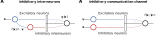
\includegraphics[trim=0cm 0cm 7.9cm 0cm,clip]{media/chapters/03_nlif/03_02/inhibitory_interneurons_overview.pdf}\hspace{0.4204cm}%
	\includegraphics[trim=0cm 0cm 7.9cm 0cm,clip]{media/chapters/03_nlif/03_02/inhibitory_interneurons.pdf}%
	{\phantomsubcaption\label{fig:inhibitory_interneurons_a}}%
	{\phantomsubcaption\label{fig:inhibitory_interneurons_b}}%
	\caption[Inhibitory interneurons]{Inhibitory interneurons.
	\textbf{(A)} To establish interneuron populations, we compute the identity function $f(x) = x$ in the purely excitatory projection onto the interneurons.
	The desired $\phi(\vec x)$ is then decoded from a virtual population encompassing both the inhibitory interneurons, and the excitatory pre-neurons.
	\textbf{(B)} Using this scheme, we can compute linear and nonlinear functions $\phi(x)$.
	Data for $100$ neurons per population with maximum firing rates between $50$ and $100\,\mathrm{Hz}$; weight matrices are determined by solving \cref{eqn:decode_nonneg} with $\sigma = 10$.
	The dotted line is the target $\phi(x)$, black line is the median decoded value over 1000 trials, shaded grey areas correspond to the 10th and 90th percentiles.
	Errors $E$ are the mean \NRMSE with standard deviation.
	}
	\label{fig:inhibitory_interneurons}
\end{figure}

\subsubsection{Inhibitory interneuons}
Connectivity patterns in biology do not suggest an arbitrary split of neural ensembles into excitatory and inhibitory neurons.
Instead, as we explained in \Cref{sec:nef_limitations}, excitatory signals are often mediated through interneurons that provide local inhibition \citep[e.g.,][Chapter~2]{kandel2012principles}.
\citet{parisien2008solving} suggest a way to 
construct \NEF networks with such inhibitory interneurons.

The techniques we discussed above can similarly be used to construct networks with inhibitory interneurons, albeit in a much simpler manner.
Recall that we can compute the identity function over purely excitatory connections (cf.~\Cref{fig:nonnegative_experiments}).
We can hence represent $\vec x$ in the interneurons using excitatory connection weights (cf.~\Cref{fig:inhibitory_interneurons_a}).
With this connection in place, the pre- and interneurons can be thought of as forming a \enquote{virtual pre-population} representing the same quantity $\vec x$.
Using \cref{eqn:decode_nonneg} we can solve for excitatory weights $\vec w_i^+$ originating from the pre-population, and inhibitory weights $\vec w_i^-$ originating from the interneurons, that project onto the post-population while approximating a function $\phi(\vec x)$.

Although we decode from multiple pre-populations, we do not need to resort to an optimisation problem such as \cref{eqn:decode_current_additive}, where we decoded additive functions from multiple pre-populations.
This is possible because both pre-populations represent the same value.
Hence, we do not require a double integral, and we can compute nonlinear functions over $\vec x$.

As depicted in \Cref{fig:inhibitory_interneurons_b}, we can use this technique to approximate linear and nonlinear functions $\phi(\vec x)$; errors mostly stem from the pre- to interneuron connection.
Crucially, in contrast to the \enquote{Parisien transform}, we did not take any special precautions regarding the interneuron tuning curve distributions.
All populations use the \enquote{standard} tuning with uniform $x$-intercepts.
This is possible because we solve for weights directly in current space.

\begin{figure}
	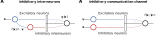
\includegraphics[trim=7.9cm 0cm 0cm 0cm,clip]{media/chapters/03_nlif/03_02/inhibitory_interneurons_overview.pdf}%
	\includegraphics[trim=7.9cm 0cm 0cm 0cm,clip]{media/chapters/03_nlif/03_02/inhibitory_interneurons.pdf}%
	{\phantomsubcaption\label{fig:inhibitory_comm_a}}%
	{\phantomsubcaption\label{fig:inhibitory_comm_b}}%
	\caption[Inhibitory communication channels]{Inhibitory communication channels.
	\textbf{(A)}~Inhibitory neurons can be used to form a communication channel, as long as there is some excitatory population that can provide a bias.
	\textbf{(B)}~Experiment demonstrating the use of this network setup as a communication channel.
	While the inhibitory connection is a good communication channel, nonlinear functions can only be computed with larger errors.
	All points are sampled from $(x, \nu) \in [-1, 1]^2$; the $\nu$-dimension is not depicted.
	See \Cref{fig:inhibitory_interneurons_b} for the network parameters and description of the depicted quantities.
	}
	\label{fig:inhibitory_comm}
\end{figure}

\subsubsection{Inhibitory communication channels}
Curiously, using the same techniques, we can also construct purely inhibitory communication channels---at least under the assumption that there is some separate excitatory pre-population that can be used as a bias source.
The lack of such an excitatory population is exactly what prevented us from computing functions across inhibitory connections in \Cref{fig:nonnegative_experiments}.

Given an inhibitory population representing $\vec x$, and another population representing some unrelated $\vec \nu$ (cf.~\Cref{fig:inhibitory_comm_a}).
Similar to \cref{eqn:decode_current_additive}, we minimise (without regularisation)
\begin{align}
	\min_{\vec w_i^+, \vec w_i^-}
	\frac{1}{\vol(\Xrepr)^2} \! \iint_{\Xrepr}
	\left(
		J_i\bigl(\langle \vec e_i, \phi(\vec x) \rangle\bigr)
		- \langle \vec w^-_i, -\vec a^-(\vec x) \rangle
		- \langle \vec w^+_i, \vec a^+(\vec \nu) \rangle
	\right)^2 \, d\vec x \, d\vec \nu %+ \sigma^2 \|\vec w_{i}^+\|_2^2 + \sigma^2 \|\vec w_{i}^-\|_2^2 \,,
	\label{eqn:inhibitory_communication_channel}
\end{align}
subject to $\vec w_{i}^+$, $\vec w_{i}^- > 0$.
Crucially, we ignore $\vec \nu$ in our target function; we solely use the pre-population to provide background activity but ignore its represented value.

Results of an experiment exploring this technique are depicted in \Cref{fig:inhibitory_comm_b}.
While computing the identity function---i.e., constructing a pure communication channel---works well, nonlinear functions can only be decoded with a considerable error, just as with purely excitatory connections channels (cf.~\Cref{fig:nonnegative_experiments}).
This is due to the standard \NEF pre-population tuning curves not providing a good basis for nonnegative decoding of many nonmonotonic functions.
In principle, it should be possible to have pre-population tuning such that any nonnegative target current function can be nonnegatively decoded with an arbitrarily small error.
An example would be the Gaussian tuning curves similar to those depicted in \Cref{fig:bias_decoding_impact_c}.

Inhibitory networks similar to what we discussed here are explored in some more detail by \citet{tripp2016function}.
However, as with the Parisien transform, this prior work relies on specific tuning of the inhibitory neurons, as well as intrinsic biases.

\subsection{Subthreshold Relaxation}
\label{sec:nef_subthreshold}

\begin{figure}
	\includegraphics{media/chapters/03_nlif/03_02/subthreshold_illustration.pdf}%
	{\phantomsubcaption\label{fig:subthreshold_illustration_a}}%
	{\phantomsubcaption\label{fig:subthreshold_illustration_b}}%
	{\phantomsubcaption\label{fig:subthreshold_illustration_c}}%
	\caption[Illustration of the goal of subthreshold relaxation]{Illustration of the goal of subthreshold relaxation.
	\textbf{(A)} Most neurons act as rectifiers. Input currents below $J_\mathrm{th}$ (grey) are mapped onto zero.
	\textbf{(B)} Five randomly generated tuning curves with uniform $x$-intercepts and maximum firing rates between $50$ and $100$ spikes per second.
	\textbf{(C)} Using affine current-translation functions $J_i(\xi)$, these tuning curves are generated by comparably large negative currents. However, the magnitude of the currents below $J_\mathrm{th}$ (grey) has no effect on the output rate; in fact any current below $J_\mathrm{th}$ has the same effect on the firing rate of the neuron.
	}
\end{figure}

Most biological model neurons act as rectifiers.
That is, input currents below a certain, usually positive, threshold $J_\mathrm{th}$ do not result in any output activity.
In the case of our simplified \LIF neuron model (cf.~\Cref{sec:simplified_neuron_models}), the threshold current $J_\mathrm{th}$ is \SI{1}{\nano\ampere} (\Cref{fig:subthreshold_illustration_a}).
We did not take this into account in our above current-space optimisation schemes.

To the contrary, our current-based loss functions in \cref{eqn:decode_current,eqn:decode_nonneg} aim at \emph{precisely} evoking certain post-synaptic currents $J_\mathrm{tar}$.
Notably, the negative currents required by the affine current translation function $J_i(\xi)$ can be larger in magnitude than the positive currents (\Cref{fig:subthreshold_illustration_b,fig:subthreshold_illustration_c}).
This has not been an issue in \NEF networks with intrinsic current-translation, as $J_i(\xi)$ takes care of appropriately scaling and offsetting the input currents.

However, in the context of our current-space optimisation schemes, a regularised least-squares optimisation problem can \enquote{prioritise} solving for exact (but irrelevant) subthreshold currents over solving for the (relevant) superthreshold currents.
This can lead to an increase in the superthreshold current-decoding error, and thus also increase the representation error in the post-population.
Additionally, as we will see below, dendritic nonlinearities impose asymptotic maximum and minimum post-synaptic currents.
Trying to solve for large negative currents may thus result in large connection weights.

One way to work around this issue is to clamp target currents $J_\mathrm{tar}$ that are substantially below the threshold to some constant.
For example, in the case of our simplified \LIF neuron, we could clamp all negative target currents to a current of zero.
This way, the solver does not have to generate the afforementioned large negative subthreshold currents.
Still, this \enquote{clamping} approach requires the weight solver to \emph{precisely} solve for the desired target current although \emph{any} subthreshold current would do.

Conceptually, it would be better to \enquote{relax} the requirement to solve for $J_\mathrm{tar}$ as precisely as possible for subthreshold currents.
Instead, we could merely demand that subthreshold target currents are decoded as subthreshold currents, regardless of the magnitude.
If this constraint is violated, i.e., if the target current $J_\mathrm{tar}$ is below the threshold and the decoded current $J_\mathrm{dec}$ is above the threshold $J_\mathrm{th}$, we measure the distance to the threshold, and not the distance to $J_\mathrm{tar}$ as an error.
We formalise this as a superthreshold error function $\mathcal{E}$,
\begin{align}
\mathcal{E}(J_\mathrm{tar}, \, J_\mathrm{dec}) = \begin{cases}
0 & \text{if } J_\mathrm{tar} < J_\mathrm{th} \text{ and } J_\mathrm{dec} < J_\mathrm{th} \,,\\
J_\mathrm{dec} - J_\mathrm{th} & \text{if } J_\mathrm{tar} < J_\mathrm{th} \text{ and } J_\mathrm{dec} > J_\mathrm{th} \,,\\
J_\mathrm{dec} - J_\mathrm{tar} & \text{if } J_\mathrm{tar} \geq J_\mathrm{th} \,,\\
\end{cases}
\label{eqn:subthreshold_error}
\end{align}
and define a new current-space optimization problem akin to \cref{eqn:decode_nonneg}
\begin{align}
	\min_{\vec w_i^+, \vec w_i^-} 
	\frac{1}{\vol(\Xrepr)}
	\int_{\Xrepr} \mathcal{E}\left( 
		J_i(\langle \vec e_i, \phi(\vec x)\rangle),
		\langle \vec w_i^+, \vec a^+(\vec x) \rangle +
		\langle \vec w_i^-, -\vec a^-(\vec x) \rangle
	\right)^2 \, d\vec x
	+ \sigma^2 \| \vec w^+_i \|_\mathrm{2}^2
	+ \sigma^2 \| \vec w^-_i \|_\mathrm{2}^2\,.
\label{eqn:decode_current_subthreshold}
\end{align}

\subsubsection{Subthreshold relaxation as a quadratic program}
It is not immediately clear how to solve this optimisation problem.
While, it is always possible to resort to gradient descent, \cref{eqn:decode_current_subthreshold} can be solved more efficiently by rewriting the loss function in terms of a convex \qprog (\QP).
\QPpl are a generalisation of least-squares and defined as follows:
\begin{definition}[Quadratic Program]
\label{def:qp}
A \emph{quadratic program} (\QP) is an optimisation problem of the form \citep[adapted in slightly simplified form from][Section~4.4]{boyd2004convex}
\begin{align*}
	\text{minimize} &\quad
		\vec \omega^T \mat P \vec \omega + \mat q^T \vec \omega \\
	\text{subject to} &\quad
		\mat G \vec \omega \leq \vec h \,,
\end{align*}
where $\vec \omega \in \mathbb{R}^{n}$, $\mat G \in \mathbb{R}^{n \times n}$, $\vec p \in \mathbb{R}^{n}$, $\mat H \in \mathbb{R}^{\ell \times n}$, $\vec q \in \mathbb{R}^{\ell}$.
Here, $n$ is the number of variables and $\ell$ is the number of inequality constraints.
If $\vec x^T \mat P \vec x$ is a convex function (i.e., if $\mat P$ is positive definite).
%and the constraints $\mat G\vec x \leq \vec h$ form a convex polytope, then the QP is \emph{convex}.
\end{definition}

Convex \qprogpl can be solved in polynomial time \citep{kozlov1980polynomial}.
There are free and open-source software libraries, such as \enquote{cvxopt} \citep{vandenberghe2010cvxopt} and \enquote{OSQP}  \citep{stellato2020osqp} that solve such problems efficiently.
In our experiments we mostly rely on OSQP.%
\footnote{Some experiments were conducted before OSQP was published; we used cvxopt in those experiments. We did not observe any discernible difference in the solutions produced by the two libraries, but as a C library using more modern algorithms, OSQP is substantially faster than the older Python library cvxopt.}

To transform a discretised version of \cref{eqn:decode_current_subthreshold} into a \qprog we split the sample points $\vec x_k$ according to whether they evoke super- or subthreshold currents.
Specifically, we arrange the pre-activities $\mat A$ and target currents $\mat J$ as follows:
\begin{align*}
	\mat{A}_\mathrm{sup} = (
		  \mat{A}^+_\mathrm{sup}, 
		- \mat{A}^-_\mathrm{sup})
		\in
		\mathbb{R}^{N_\mathrm{sup} \times (n^+ + n^-)} \,,
	&&
	\mat{J}_\mathrm{sup} \in \mathbb{R}^{N_\mathrm{sup}} \,,
	&&
	\mat{A}_\mathrm{sub} = (
		  \mat{A}^+_\mathrm{sub}, 
		- \mat{A}^-_\mathrm{sub})
		\in
		\mathbb{R}^{N_\mathrm{sub} \times (n^+ + n^-)} \,.
\end{align*}
Here, $N_\mathrm{sup}$, $N_\mathrm{sub}$ with $N = N_\mathrm{sup} + N_\mathrm{sup}$
are the number of samples with a super- and subthreshold target currents, and, as before, $n^+$ and $n^-$ correspond to the number of excitatory and inhibitory pre-neurons.
Using these matrices, \cref{eqn:decode_current_subthreshold} can be expressed as a \QP by letting
\begingroup
\setlength\fboxsep{2pt}
\newcommand{\cA}{LightSkyBlue}
\newcommand{\cB}{Plum}
\newcommand{\cC}{Salmon}
\newcommand{\cD}{Khaki}
%\newcommand{\hlA}[1]{\colorbox{\cA}{\ensuremath{#1}}}
%\newcommand{\hlB}[1]{\colorbox{\cB}{\ensuremath{#1}}}
%\newcommand{\hlC}[1]{\colorbox{\cC}{\ensuremath{#1}}}
%\newcommand{\hlD}[1]{\colorbox{\cD}{\ensuremath{#1}}}
\newcommand{\hlA}[1]{{\ensuremath{#1}}}
\newcommand{\hlB}[1]{{\ensuremath{#1}}}
\newcommand{\hlC}[1]{{\ensuremath{#1}}}
\newcommand{\hlD}[1]{{\ensuremath{#1}}}
\begin{align}
	\mat P &= \begin{pmatrix}
		  \hlA{(\mat A_\mathrm{sup})^T \mat A_\mathrm{sup} + N \sigma^2 \mat I)}
		& 0 \\
		  0
		& \hlB{\mat I}
	\end{pmatrix} ,
	&
	\!\!\! \vec q &= \begin{pmatrix}
		\hlA{(\mat A_\mathrm{sup})^T \vec J_\mathrm{sup}} \\
	0
	\end{pmatrix} ,
	&
	\!\!\! \mat G &= \begin{pmatrix}
		\hlC{\mat A_\mathrm{sub}} & \hlB{\mat I} \\
		\hlD{-\mat I} & 0
	\end{pmatrix} ,
	&
	\!\!\! \vec h &= \begin{pmatrix}
		\hlC{\vec{J}_\mathrm{th}} \\
		\hlD{0}
	\end{pmatrix} .
	\label{eqn:decode_subthreshold_qp}
\end{align}
The number of variables is $n = n^+ + n^- + N_\mathrm{sub}$, and the number of inequality constraints is $\ell = N_\mathrm{sub} + n^+ + n^-$.
The parameter vector $\vec \omega \in \mathbb{R}^{n}$ can be split into the excitatory and inhibitory weights $\vec w_i^+ \in \mathbb{R}^{n^+}$, $\vec w_i^- \in \mathbb{R}^{n^-}$, as well as discardable slack variables $\vec s_i \in \mathbb{R}^{N_\mathrm{sub}}$.

The rationale behind \cref{eqn:decode_subthreshold_qp} is as follows.
The first line of $\mat P$ and $\vec q$
%(${\color{\cA}\blacksquare}$)
is the standard regularised least-squares problem obtained by expanding the superthreshold potion of \cref{eqn:decode_current_subthreshold} (cf.~\cite{boyd2004convex}, Section~4.4).
The first column and row of $\mat G$ and $\vec h$
%(${\color{\cC}\blacksquare}$)
add an inequality constraint that ensures that samples with subthreshold currents are decoded as subthreshold currents.
Violations of this constraint, i.e., case two of \cref{eqn:subthreshold_error}, are enabled by the slack variables $\vec s_i$ (second column of $\mat P$ and $\mat G$%
%; ${\color{\cB}\blacksquare}$
).
These slack variables correspond to the error $J_\mathrm{th} - J_\mathrm{tar}$, which is penalised accordingly in $\mat P$.
Finally, nonnegativity of the weights is ensured by the second row of $\mat G$ and $\vec h$%
% (${\color{\cD}\blacksquare}$)
. One can easily show that this \QP is convex.
\endgroup

\begin{figure}
	\includegraphics{media/chapters/03_nlif/03_02/subthreshold_comparison.pdf}%
	{\phantomsubcaption\label{fig:subthreshold_comparison_a}}%
	{\phantomsubcaption\label{fig:subthreshold_comparison_b}}%
	{\phantomsubcaption\label{fig:subthreshold_comparison_c}}%
	{\phantomsubcaption\label{fig:subthreshold_comparison_d}}%
	\caption[Current decoding with and without subthreshold relaxation]{Current decoding with and without subthreshold relaxation in a setting with low regularisation ($\sigma = 0.31$) and few pre-neurons ($n = 50$).
	Values above each plot are the \RMS of the superthreshold error ${\mathcal{E}}$ (eq.~\ref{eqn:subthreshold_error}).
	Subthreshold relaxation substantially reduces the decoding error.	
	}
	\label{fig:subthreshold_comparison}
\end{figure}

\subsubsection{Example: Individual post-neuron}
In \Cref{fig:subthreshold_comparison} we decode the post-synaptic currents for a single post neuron using \NNLS, \NNLS with clamped target currents, and subthreshold relaxation.
At least in this example, subthreshold relaxation substantially reduces the superthreshold decoding error.
In contrast, clamping the target currents has only a limited positive effect.
Notably, and particularly pronounced in the case of purely excitatory pre-neurons, the solution obtained with subthreshold relaxation is supported by more pre-neurons.
This is visible in \Cref{fig:subthreshold_comparison_c}, where subthreshold relaxation decodes a non-zero current for negative $\xi$, resulting in a smaller regularisation error (i.e., weight \RMS of $0.8 \times 10^{-3}$ vs. $2 \times{10}^{-3}$).

\begin{figure}[t]
	\includegraphics{media/chapters/03_nlif/03_02/subthreshold_experiment.pdf}%
	{\phantomsubcaption\label{fig:subthreshold_experiment_a}}%
	{\phantomsubcaption\label{fig:subthreshold_experiment_b}}%
	{\phantomsubcaption\label{fig:subthreshold_experiment_c}}%
	\caption[Reduction in decoding error achieved with subthreshold relaxation]{Reduction in decoding error achieved with subthreshold relaxation compared to standard \NNLS and clamping the target current.
	\textbf{(A)} Reduction in the decoded post-synaptic currents error relative to \NNLS for different thresholds in the error measure $\mathcal{E}$.
	Each box plot over three functions, $100$ random networks, $11$ noise magnitudes, and $9$ random samplings of the noise ($N = 29\,700$); whiskers are the extrema, boxes the quartiles, orange line is the median, green dashed line the mean.
	\textbf{(B)}
	Same as \emph{(A)}, but for the post-population decoding error.
	\textbf{(C)} Same data as above, but over different pre-population noise magnitudes and for different functions $\phi(x)$ computed in the pre to post connection.
	Coloured lines show the median error (see \emph{(A, B)} for a legend); shaded areas are the 25\% and 75\% quartiles.
	}
	\label{fig:subthreshold_experiment}
\end{figure}

\subsubsection{Systematic experiment}
One issue with subthreshold relaxation is that not solving for strongly negative currents can result in a narrower separation boundary between the threshold and the decoded current.
Hence, noise on the pre-activities is more likely to result in positive post-activity.
However, this may be compensated for by the smaller regularisation error, and hence higher robustness to noise as observed in the previous example.

\Cref{fig:subthreshold_experiment} depicts the results of a more systematic experiment.
We compute three polynomials in the connection between one hundred pre and post \LIF rate neurons ($1\!\!:\!\!1$ excitatory to inhibitory ratio) with varying degree of Gaussian noise added to the pre-activities.
We select the regularisation factor $\sigma$ to minimize the error for the given amount of noise on a separate training set.
We furthermore vary the threshold $J_\mathrm{th}$ assumed in \cref{eqn:subthreshold_error}, to investigate the effect of moving $J_\mathrm{th}$ away from the true threshold.

As visible in \Cref{fig:subthreshold_experiment_a}, subthreshold relaxation reduces the current decoding error by about 50\% (median), largely independent of the assumed $J_\mathrm{th}$.
Clamping the currents leads to a reduction in error with a median of about 35\%, but, overall, the reduction in error is less consistent.
Improvements to the representation accuracy (\Cref{fig:subthreshold_experiment_b}) are less drastic, with the largest improvement for $J_\mathrm{th} = \SI{0.75}{\nano\ampere}$ with a median reduction in error of about 13\%.
This confirms our suspicion that setting $J_\mathrm{th}$ to the true threshold can be slightly detrimental.

This is further confirmed by the experiment in \Cref{fig:subthreshold_experiment_c} where we plot the post-population representation error over different pre-activity noise magnitudes.
For small amounts of noise subthreshold relaxation with $J_\mathrm{th} = \SI{1}{\nano\ampere}$ can lead to large improvements in the representation error; however, for larger noise magnitudes the overall benefit of subthreshold relaxation is smaller, with slightly reduced $J_\mathrm{th}$ performing the best.
%We provide additional results from this experiment in Appendix C.2.

Keep in mind that \LIF rate neurons are a worst-case scenario with respect to sensitivity to pre-activity noise injected near the threshold.
\LIF rate neurons possess a very steep activity onset, where small changes in current lead to large fluctuations in activity.
This tends to be less of an issue with transient noise in spiking neural networks, which results in a smoother response curve (see our discussion below, as well as \cite{hunsberger2015spiking}).
We can thus expect that, in practice, the impact of subthreshold relaxation is somewhere between the values obtained for the current decoding and representation error.

\subsection{Extension Toward Dendritic Nonlinearities}
\label{sec:nef_nonlinear}

Up to this point we assumed current-based synapses.
As previously discussed in \Cref{sec:dendritic_computation_theory}, the defining property of current-based synapses is that the somatic current $J$ is linear in the synaptic weights $\vec w$ and the pre-synaptic activities $\vec a$, that is $a_i = G[J] = G[\langle \vec w, \vec a \rangle]$.
In contrast, we described neurons with nonlinear synapses as follows
\begin{align}
	a_i &=
	\mathscr{G} \bigl[
		g_i^1, \ldots, g_i^k
	\bigr] =
	\mathscr{G} \bigl[
		\langle \vec w_{i}^1, \vec a_1 \rangle,
		\ldots ,
		\langle \vec w_{i}^k, \vec a_k \rangle
	\bigr] \,.
	\label{eqn:def_response_curve_g}
\end{align}
Here, $k$ is the number of input channels, and the vector $\vec g_i = (g^1_i$, $\ldots$, $g^k_i)$ describes some abstract \enquote{channel state}.
Again, we assume that, on average, each channel state $g^j_i$ is linear in the weights and the activities $\vec a_j$ of the neurons connecting to the $j$th channel.
However, we do not make any assumption regarding the effect of $g^j_i$ on the somatic current $J$; more fundamentally, we do not assume that there exists an easily identifiable somatic current at all.

The lack of an identifiable somatic current makes it more challenging to integrate such neurons into the \NEF.
The optimisation problems we discussed in this section relied on the current translation function $J_i(\xi)$ to enforce the normative tuning constraint $a_i(\vec x)$.
Of course, as mentioned above, we could resort to gradient descent to optimise \cref{eqn:dendritic_computation_optimisation}.
However, our current-based optimisation schemes work well in that they allow us to quickly solve for globally optimal weights.
As we will see, it is still possible to perform global current-space optimisation for some multi-channel neurons.
Additionally, we can use the same ideas to iteratively solve for locally optimal weights in more complex multi-compartment neurons.

\begin{figure}
	\centering
	\includegraphics{media/chapters/03_nlif/03_02/two_compartment_response_curve.pdf}
	\caption[Neural response curve decomposition]{Neural response curve decomposition. \textbf{(A)} Illustration of the multivariate neuron response curve $\mathscr{G}(g_\mathrm{E}, g_\mathrm{I})$ for a two-compartment \LIF neuron with excitatory and inhibitory conductance-based channels. \textbf{(B, C)} The chosen somatic nonlinearity $G$ and its inverse $G^{-1}$. \textbf{(D)} corresponding input-dependent nonlinearity $H$. The neuron does not fire in the hatched regions, that is, $G^{-1}$ is ill-defined.} 
	\label{fig:two_compartment_response_curve}
\end{figure}

To this end, the crucial idea is to mathematically reintroduce a \enquote{virtual} somatic current $J$ by decomposing $\mathscr{G}$ into the standard somatic nonlineartiy $G$ and a dendritic nonlinearity $H$.

\begin{definition}[Dendritic Nonlinearity]
\label{def:dendritic_nonlinearity}
Given a neural response curve $G$, the \emph{dendritic nonlinearity} $H(\vec g_i)$ of a multi-channel neuron with response curve $\mathscr{G}$ maps the input channel state $\vec g_i = (g^1_i, \ldots, g^k_i)$ onto an \emph{average}, time-independent somatic current $J$ such that
\begin{align}
		H\big(g^1_i, \ldots, g^k_i\big) = J
	\Leftrightarrow
		G\big[J\big] = \mathscr{G}\big[g^1_i, \ldots, g^k_i\big] 
	\Leftrightarrow
		\mathscr{G}\big[g^1_i, \ldots, g^k_i\big] = G\big[H(g^1_i, \ldots, g^k_i)\big] \,.
	\label{eqn:def_h}
\end{align}
\end{definition}
Optimally, $G$ is chosen such that $H$ is as simple as possible.
For example, if the neuron model is an extension to a \LIF neuron, $G$ can be the standard \LIF response curve.
In this case, $H$ translates the input into an \enquote{\LIF-equivalent current}.
In the trivial case of the above current-based \LIF neurons with excitatory and inhibitory inputs, we would obtain $H(J_\mathrm{E}, J_\mathrm{I}) = J_\mathrm{E} - J_\mathrm{I}$.

We use the dendritic nonlinearity $H$ to define a new current-space loss
\begin{align}
	E = \frac{1}{\vol(\Xrepr)} \int_{\Xrepr}
		\mathcal{E} \bigl(
			J_i(\langle \vec e_i, f(\vec x_k) \rangle),
			H(\langle \vec w^1_i, \vec a^k \rangle, \ldots, \langle \vec w^k_i, \vec a^k \rangle)
		\bigr)^2 \,\mathrm{dx} + \sigma^2 \sum_{j = 1}^\ell \| \vec w^j_i \|_2^2\,,
\label{eqn:decode_nonlinear_synapses}
\end{align}
where $\mathcal{E}$ is the superthreshold error defined in \cref{eqn:subthreshold_error}, $\vec a^j$ are the pre-activities connection, and weights $\vec w_i$ may be---depending on the input channel type---nonnegative.

We next show that it is possible to derive $H$, or at least a suitable surrogate model, in closed form for multi-compartment \LIF neurons with conductance-based synapses.
If $H$ cannot be derived in closed form, we can sample $\mathscr{G}$ over varying synaptic states and, as depicted in \Cref{fig:two_compartment_response_curve}, compute $H$ indirectly by applying an inverse mapping $G^{-1}$ to the recorded data.

%
%\clearpage
%\setcounter{section}{2}
%% !TeX spellcheck = en_GB

\section{A Family of Multi-Compartment LIF Neurons}
\label{sec:nlif}

The dendritic nonlinearity $H$ introduced in the last section maps some channel state $\vec g$ onto an average somatic current.
While this mapping can always be established numerically, expressing $H$ in closed form has the potential to simplify the optimisation problem in \cref{eqn:decode_nonlinear_synapses}.

In this section, we discuss a family of multi-compartment \LIF neurons that we refer to as \enquote{\nlif}.
These neuron models are based on the multi-compartment neurons that we reviewed in \Cref{sec:comp}, and, as we discussed in the introduction of this chapter, were constructed with mathematical tractability in mind, rather than biological detail.
While it is not possible to derive an exact dendritic nonlinearity $H$ for these neurons, we derive a closed-form \enquote{surrogate} model of $H$ that can be fit to numerical data.

\subsection{Mathematical Description of $n$-LIF Neurons}
\label{sec:nlif_description}

\begin{figure}
	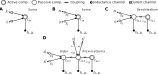
\includegraphics{media/chapters/03_nlif/03_03/multi_compartment_examples.pdf}%
	{\phantomsubcaption\label{fig:nlif_a}}%
	{\phantomsubcaption\label{fig:nlif_b}}%
	{\phantomsubcaption\label{fig:nlif_c}}%
	{\phantomsubcaption\label{fig:nlif_d}}%
	{\phantomsubcaption\label{fig:nlif_e}}%
	\caption[\enquote{Ball-and-stick} illustration of multi-compartment LIF neurons]{\enquote{Ball-and-stick} illustration of multi-compartment \LIF neurons.
	Large circles correspond to compartments, small circles and rectangles to conductance- and current-based channels. Filled symbols indicate passive channels.
	\textbf{(A)} Standard \LIF neuron with current-based inputs.
	\textbf{(B)} \LIF neuron with conductance-based input channels.
	\textbf{(C)} Two-compartment neuron with a separate dendritic compartment.
	\textbf{(D, E)} Three- and four-compartment \LIF neurons with apical and basal dendrites.}
	\label{fig:nlif}
\end{figure}

We define an \nlif neuron as a connected graph of resistively coupled capacitive compartments.
Each neuron possesses exactly one active compartment with standard \LIF dynamics, while the other compartments represent a passive dendritic tree.
Each compartment may hold any number of passive current- and conductance-based channels.
Channels are either constant (representing bias currents and leak channels), or receive external input (representing synapses).
Examples of such neurons are depicted in \Cref{fig:nlif} using a \enquote{ball-and-stick} representation.

As a point of reference, the expanded equivalent circuit diagram of the two-compartment neuron with conductance-based synapses (\Cref{fig:nlif_c}) is depicted in \Cref{fig:two_comp_lif_circuit}.
This particular model has originally been described by \citet{vu1993mechanism} and was subsequently discussed by \citet{koch1999biophysics} and \citet{capaday2006direct}.
We discuss this model in more detail in the next section, and for now focus on \nlif neurons in general.

\begin{figure}
	\includegraphics{media/chapters/03_nlif/03_03/neuron_model_trace_composite.pdf}%
	{\phantomsubcaption\label{fig:two_comp_lif_circuit}}
	{\phantomsubcaption\label{fig:two_comp_lif_trace}}
	\caption[Circuit and membrane potential trace of a two-compartment LIF neuron]{Circuit and membrane potential trace of a two-compartment neuron.
	\textbf{(A)} Circuit diagram corresponding to the model in \Cref{fig:nlif_c}.
	\textbf{(B)} Membrane potential traces for both compartments for a small constant excitatory input.
	Notice how the explicit spike model in the somatic compartment (\emph{top}) influences the membrane potential of the dendritic compartment (\emph{bottom}).}
	\label{fig:two_comp_lif}
\end{figure}

\subsubsection{Superthreshold dynamics}
In contrast to the standard \LIF model (cf.~Section~2.2.3), the active \nlif compartment possess an explicit spike model.
% TODO: Add correct reference
As pointed out by \citet{capaday2006direct}, this is important in multi-compartment models, since the spike potential causes a substantial current to flow into the dendritic compartments (cf.~\Cref{fig:two_comp_lif_trace}).

More precisely, we model the superthreshold dynamics as follows.
Whenever the membrane potential \vMem surpasses the threshold $v_\mathrm{th}$, \vMem is clamped to a \enquote{spike potential} $v_\mathrm{spike}$ for a period $\tau_\mathrm{spike}$ and subsequently forced to $v_\mathrm{reset}$ for the refractory period $\tau_\mathrm{ref}$.
Unless specified otherwise, we use $\tau_\mathrm{spike} = \SI{1}{\milli\second}$ and $\tau_\mathrm{ref} = \SI{2}{\milli\second}$ in our models.

\subsubsection{Subthreshold dynamics}
The dynamics of the $i$th compartment are
\begin{align}
	\Cmi \frac{d}{dt} \vMemi(t) &=
		\sum_{k=1}^{M_i} g_k^i(t) \bigl( E_k^i - \vMemi(t) \bigr) +
		\sum_{k=1}^{N_i} J_k^i(t) +
		\sum_{j=1}^{n} \bigl(\vMemj(t) - \vMemi(t)\bigr) \cij \,,
\label{eqn:nlif_single_compartment}
\end{align}
where \Cmi is the membrane capacitance of the compartment, $M_i$ and $N_i$ are the number of conductance- and current-based channels, respectively, $g_{k}^i(t)$ is the momentary conductance of the $k$th conductance-channel with reversal potential $E_{k}^i$, and $J_{k}^i(t)$ is the current injected into the current-based channel $j$.
Finally, \cij is the coupling conductance between the $i$th and the $j$th compartment.
The adjacency matrix of coupling conductances $\mat C$ must be symmetric, and the connectivity graph encoded by $\mat C$ must have exactly one connected component (cf.~our discussion in Section~2.2.3).
%TODO: Correct reference
Some conductances $g_{k}^i(t)$ and currents $J_{k}^i(t)$ are constant, such as the static leak channels and bias currents.

\begin{table}
	\caption[Matrix representations of the first four neuron models in \Cref{fig:nlif}]{Matrix representations of the first four neuron models in \Cref{fig:nlif}. See text for details.
	%All matrices are multiplied by the membrane capacitance $C_\mathrm{m}$ (assuming that $C_\mathrm{m}$ is the same across compartments).
	}
	\label{tbl:nlif_matrices}
	\small\sffamily\centering
	\begin{tabular}{c c c c c c}
		\toprule
		\multicolumn{1}{c}{\textbf{Model}} & \vnap & \mnAp & \vnbp & \mnBp & \mnL \\
		\midrule
		%\cmidrule{1-1}\cmidrule(l){2-6}
			\textbf{(A)}
			& $\displaystyle \begin{bmatrix} g_\mathrm{L} \end{bmatrix}$
			& $\displaystyle \begin{bmatrix} 0 & 0 \end{bmatrix}$
			& $\displaystyle \begin{bmatrix} g_\mathrm{L} E_\mathrm{L} \end{bmatrix}$
			& $\displaystyle \begin{bmatrix} 1 & -1 \end{bmatrix}$
			& $\displaystyle \begin{bmatrix} 0 \end{bmatrix}$\\[0.5cm]
			\textbf{(B)} 
			& $\displaystyle \begin{bmatrix} g_\mathrm{L} \end{bmatrix}$
			& $\displaystyle \begin{bmatrix} 1 & 1 \end{bmatrix}$
			& $\displaystyle \begin{bmatrix} g_\mathrm{L} E_\mathrm{L} \end{bmatrix}$
			& $\displaystyle \begin{bmatrix} E_\mathrm{E} & E_\mathrm{I} \end{bmatrix}$
			& $\displaystyle \begin{bmatrix} 0 \end{bmatrix}$ \\[0.5cm]
			\textbf{(C)} 
			& $\displaystyle \begin{bmatrix}
				g_\mathrm{L} \\ g_\mathrm{L}
			\end{bmatrix}$
			& $\displaystyle \begin{bmatrix} 0 & 0 \\
				1 & 1 \end{bmatrix}$
			& $\displaystyle \begin{bmatrix}
				g_\mathrm{L} E_\mathrm{L} \\
				g_\mathrm{L} E_\mathrm{L}
			\end{bmatrix}$
			& $\displaystyle \begin{bmatrix}
				0 & 0 \\
				E_\mathrm{E} & E_\mathrm{I}
			\end{bmatrix}$
			& $\displaystyle \begin{bmatrix} c_{12} & -c_{12} \\ -c_{12} & c_{12} \end{bmatrix}$ \\[0.5cm]
			\textbf{(D)} 
			& $\displaystyle \begin{bmatrix}
				g_\mathrm{L} \\
				g_\mathrm{L} \\
				g_\mathrm{L}
			\end{bmatrix}$
			& $\displaystyle \begin{bmatrix}
			    0 & 0 & 0 & 0\\
				1 & 1 & 0 & 0 \\
				0 & 0 & 1 & 1 \end{bmatrix}$
			& $\displaystyle \begin{bmatrix}
				g_\mathrm{L} E_\mathrm{L} \\
				g_\mathrm{L} E_\mathrm{L} \\
				g_\mathrm{L} E_\mathrm{L}
			\end{bmatrix}$
			& $\displaystyle \begin{bmatrix}
				0 & 0 & 0 & 0 \\
				E_\mathrm{E} & E_\mathrm{I} & 0 & 0 \\
				0 & 0 & E_\mathrm{E} & E_\mathrm{I} \\
			\end{bmatrix}$
			& $\displaystyle \begin{bmatrix} c_{12} & -c_{12} & 0 \\ -c_{12} & c_{12} + c_{23} & -c_{23} \\ 0 & -c_{23} & c_{23} \end{bmatrix}$ 			\\
		\bottomrule
	\end{tabular}
\end{table}

\subsubsection{Canonical matrix form}
We can rearrange \cref{eqn:nlif_single_compartment} to \emph{resemble} a canonical \LTI system.%
\footnote{
In general, \cref{eqn:nlif_matrix} is \emph{not} a linear dynamical system.
However, there are two conditions under which this system is linear: either $\vng(t)$ is constant, or there are no product terms between $\vng(t)$ and $\vvMem(t)$.
This is the case if the system has no conductance-based input channels and \mnAp is zero.
Note that the constant offset \vnbp in \cref{eqn:nlif_matrix} does not make the dynamical system non-linear, but merely mandates one auxiliary dimension.
}
Let $k$ be the number of non-static input channels, and $\vng \in \mathbb{R}^k$ a vector representing the all input channel states, that is, all non-static conductances $g_{ij}$ and currents $J_{ij}$.
This channel state is generally linear in the synaptic weights and the pre-activities (cf.~\Cref{sec:nef_nonlinear}).
We have
\begin{align}
	\frac{d}{dt} \vCm \circ \vvMem(t)
	&= \mnA\bigl[\vng(t)\bigr] \vvMem(t) + \vnb\bigl[\vng(t)\bigr]
	 = -\bigl[\mnL + \mathrm{diag}\bigl(\vnap + \mnAp \vng(t)\bigr)\bigr] \vvMem(t) + \big[\vnbp + \mnAp \vng(t)\big] \,.
	\label{eqn:nlif_matrix}
\end{align}
Here, $\vCm \in \mathbb{R}^n$ is a vector of membrane capacitances, \enquote{$\circ$} denotes elementwise multiplication, $\mnA[\vng(t)] \in \mathbb{R}^{n \times n}$ is the \enquote{voltage feedback matrix}, and $\vnb[\vng(t)] \in \mathbb{R}^n$ describes the input to the system.
We further decompose \mnA, \vnb into input-independent and input-dependent terms.
The Laplacian $\mnL \in \mathbb{R}^{n \times n}$ and the vectors $\vnap \in \mathbb{R}^n$, $\vnbp \in \mathbb{R}^n$ describe the input-independent portions of the system, whereas the matrices $\mnAp \in \mathbb{R}^{n \times k}$ and $\mnBp \in \mathbb{R}^{n \times k}$ describe its input-dependent parts.

More specifically, the Laplacian \mnL is the difference between the weighted degree matrix and the adjacency matrix, and, in our case, is given as $\mnL = \diag(\mC \mat I) - \mC$.%
\footnote{Indeed, the graph Laplacian is often motivated in textbooks with electrical networks similar to the one discussed here; in this context it is also referred to as the \enquote{Kirchhoff matrix} \citep[e.g.,][Chapter~2]{bollobas1998modern}.}
The vector \vnap consists of sums of static channel conductances for each channel (such as the leak conductance) and \vnbp contains the sums of the static channel conductances multiplied by their reversal potential.
The matrix \mnAp contains one-entries for input-variables influencing a conductance-based channel in the corresponding compartment.
\mnBp contains a \enquote{one} for each variable current-based channel in the corresponding compartment, and the reversal potential for each variable conductance-based channel in a compartment.
Examples of these matrices for the first four \nlif neuron models depicted in \Cref{fig:nlif} are given in \Cref{tbl:nlif_matrices}.

\pagebreak

\subsection{Analysis of the Subthreshold $n$-LIF Dynamics}
\label{sec:nlif_subth_properties}

The dynamics of the \nlif system are quite benign.
The system is generally stable and does not oscillate; in other words, the eigenvalues of $\mnA[\vng] \diag(\vCm)^{-1}$ are real-valued and strictly negative \citep[e.g.,][Chapter~5]{strogatz1994nonlinear}.
More formally (see \Cref{app:thm_nlif_convergence} for a proof):
\begin{restatable}{theorem}{ThmNlifConvergence}
\label{thm:nlif_convergence}
Consider an $n$-LIF neuron with at least one static conductance-based channel and any input vector \vng with non-negative entries for conductance-based input channels.
In this case, the feedback matrix $\mnA[\vng] \diag(\vCm)^{-1}$ is negative definite.
\end{restatable}
This is quite intuitive form a physical perspective.
The \nlif neuron essentially is a resistor-capacitor network.
When tying at least one point of the network to a voltage source, the capacitors will converge to some equilibrium potential $\vneq$.
For constant \vng the dynamics are
\begin{align}
	{\vMem}(t)
		&= \vneq + \exp\big(\mnA[\vng] \diag(\vCm)^{-1} t\big) \big(\vvMem(0) - \vneq\big) \,,
		& \text{where }  \vneq &= -\mnA[\vng]^{-1} \vnb[\vng] \,,
	\label{eqn:nlif_dynamics}
\end{align}
Crucially, $\mnA[\vng]$ is guaranteed to be invertible under the conditions listed in \Cref{thm:nlif_convergence}.
%It is singular exactly if the neuron does not possess any conductance-based channels, or the conductances of all channels are zero.
Furthermore, note that \vneq does not depend on \vCm; both $\mnA[\vng]$ and $\vnb[\vng]$ are divided by \vCm (cf.~eq.~\ref{eqn:nlif_matrix}):
\begin{align*}
	  \bigl(\diag(\vCm)^{-1} \mnA[\vng]\bigr)^{-1} \bigl(\diag(\vCm)^{-1} \vnb[\vng]\bigr)
	= \mnA[\vng]^{-1} \diag(\vCm) \diag(\vCm)^{-1} \vnb[\vng] = \mnA[\vng]^{-1} \vnb[\vng] \,.
\end{align*} 

\begin{figure}
	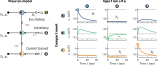
\includegraphics{media/chapters/03_nlif/03_03/nlif_impulse_response_panels.pdf}
	\label{fig:nlif_impulse_response_panels}
	\caption[Impulse response of the $n$-LIF neuron]{Impulse response of the $n$-LIF neuron.
	Injecting a pulse into a nonlinear conductance channel (injection sites \emph{1}, \emph{2}) at most charges the corresponding compartment up to the channel reversal potential.
	In contrast, current inputs (injection site \emph{3}) can charge the membrane to arbitrary potentials.
	The impulse is filtered and dampened while it is travelling through a neuron.
	}
\end{figure}
The impulse response of the system is depicted in \Cref{fig:nlif_impulse_response_panels}.
Each compartment acts as a first-order low-pass filter; the response in compartment $i$ to an impulse in compartment $j$ thus resembles a low-pass filter of order $d(i, j)$, the distance between nodes $i$, $j$.
%However, once again note that conductance channels are nonlinear---the impulse response does not fully characterise the system.
%No matter what the previous membrane potential, an input will at most charge the corresponding compartment up to the channel reversal potential.

\subsection{Deriving a Surrogate Model of the Dendritic Nonlinearity $H$}
\label{sec:nlif_derive_h}

As defined above (cf.~\Cref{def:dendritic_nonlinearity}), the dendritic nonlinearity $H$ maps a synaptic state $\vec g$ onto the synaptic current $J$ such that $G[J] = \mathscr{G}[\vec g]$, where $G[J]$ is a standard single-channel response curve and $\mathscr{G}[\vec g]$ is the response curve of the multi-channel neuron.
If, for example, $G[J]$ is the \LIF response curve, then $H$ maps $\vec g$ into an \enquote{\LIF-equivalent} current.

Trivial cases aside, it is generally not possible to provide $H$ in closed form for \nlif neurons.
This is due to the nonlinear interaction between the membrane potential and conductance-based input channels, as well as the influence of the nonlinear superthreshold dynamics on the dendritic compartments.
Still, we can derive a parametrised \enquote{surrogate model} that approximates $H$ well and that we can fit to empirical data.

\subsubsection{Subthreshold current}
As a first step toward this model, consider the case where the neuron model is purely in its subthreshold regime.
Without loss of generality, assume that the compartment with index $i = 1$ is the somatic compartment.
Furthermore, assume that this compartment possesses a leak channel with conductance $g_\mathrm{L}$ and reversal potential $E_\mathrm{L}$.
The current $H(\vec g; t)$ flowing into the somatic compartment at time $t$ for constant $\vec g$ is the differential of $v_1$ divided by the membrane capacitance, that is
\begin{align}
	H(\vec g; t) = \big(\mat A[\vec g] \vec v(t) + \vec b[\vec g] \big)_1 \,.
	\label{eqn:nlif_sub_momentary}
\end{align}
To obtain an \LIF-equivalent current, we must further subtract the leak current $g_\mathrm{L} \big( E_\mathrm{L} - v_1(t) \big)$; this current is already accounted for in the \LIF response curve $G[J]$.%
\footnote{
Of course, $H$ depends on the specific choice of $G[J]$.
For example, if we used the response curve for an non-leaky IF-neuron instead, we would not have to subtract the leak current.
More specifically, in the next section, we discuss using a rectified linear unit instead of the \LIF response curve.
Also note that, in practice, these details are not too critical.
As we discuss below, we propose use a parametrised version of $H$ that is fit to numerical measurements of $J$; this process naturally compensates for missing offsets.
}

\begin{figure}[p]
	\centering
	\includegraphics{media/chapters/03_nlif/03_03/average_som_pot.pdf}%
	{\phantomsubcaption\label{fig:avg_vsom_a}}%
	{\phantomsubcaption\label{fig:avg_vsom_b}}%
	\caption[Mean somatic membrane potential over the neuron output rate]{Mean somatic membrane potential $\vSom$ over the output rate for a current-based \LIF neuron. Lines correspond to the average potential for different pre-synaptic spike rates.
	Mean post-synaptic currents are fixed in individual trials, so the spike rate purely corresponds to the amount of noise.
	Data over 128 random Poisson spike-trains per 1000 individual mean post-synaptic currents.
	Synaptic filter time constant is $5\,\mathrm{ms}$. Shaded areas correspond to 25/75\% percentiles, lines to the mean. \textbf{(A)} Average membrane potential excluding the refractory and spike period. Dotted line is a  linear model that takes the relative length of the spike and refractory phase into account. \textbf{(B)} Average membrane potential including the refractory and spike period.}
	\label{fig:avg_vsom}
\end{figure}

\begin{table}[p]
	\caption[Reduced matrix representations of the first four neuron models in \Cref{fig:nlif}]{Reduced matrix representations of the first four multi-compartment neuron models in \Cref{fig:nlif}.
	The somatic compartment is disconnected from the remaining neuron model.
	Connections to the somatic compartment are replaced by a static conductance-based channel with reversal potential $\vSom$. The voltage difference between $\vSom$ and the equilibrium potential of the new model is proportional to the current flowing into the somatic compartment.
	}
	\label{tbl:nlif_matrices_reduced}
	\small\sffamily\centering
	\begin{tabular}{c c c c c c c}
		\toprule
		\multicolumn{1}{c}{\textbf{Model}\!\!} & $\vec{\tilde a}'$ & $\mat{\tilde A}'$ & $\vec{\tilde b}'$ & $\mat{\tilde B}'$ & $\mat{\tilde L}$ & $\vec{\tilde c}$\\
		\midrule
			\textbf{(A)}
			& $\displaystyle \begin{bmatrix} 1 \end{bmatrix}$
			& $\displaystyle \begin{bmatrix} 0 & 0 \end{bmatrix}$
			& $\displaystyle \begin{bmatrix} g_\mathrm{L} ( E_\mathrm{L} - \vSom ) + \vSom \end{bmatrix}$
			& $\displaystyle \begin{bmatrix} 1 & -1 \end{bmatrix}$
			& $\displaystyle \begin{bmatrix} 0 \end{bmatrix}$
			& $\displaystyle \begin{bmatrix} 1 \end{bmatrix}$\\[0.5cm]
			\textbf{(B)}
			& $\displaystyle \begin{bmatrix} 1 \end{bmatrix}$
			& $\displaystyle \begin{bmatrix} 0 & 0 \end{bmatrix}$
			& $\displaystyle \begin{bmatrix} g_\mathrm{L} ( E_\mathrm{L} - \vSom ) + \vSom \end{bmatrix}$
			& $\displaystyle \begin{bmatrix} E_\mathrm{E} - \vSom & E_\mathrm{I} - \vSom \end{bmatrix}$
			& $\displaystyle \begin{bmatrix} 0 \end{bmatrix}$
			& $\displaystyle \begin{bmatrix} 1 \end{bmatrix}$\\[0.5cm]
			\textbf{(C)}
			& $\displaystyle \begin{bmatrix}
				1 \\
				g_\mathrm{L} + c_\mathrm{12}
			\end{bmatrix}$
			& $\displaystyle \begin{bmatrix}
				0 & 0 \\
				1 & 1 \end{bmatrix}$
			& $\displaystyle \begin{bmatrix}
				g_\mathrm{L} ( E_\mathrm{L} - \vSom ) + \vSom \\
				g_\mathrm{L} E_\mathrm{L} + c_{12} \vSom
			\end{bmatrix}$
			& $\displaystyle \begin{bmatrix}
				0 & 0 \\
				E_\mathrm{E} & E_\mathrm{I}
			\end{bmatrix}$
			& $\displaystyle \begin{bmatrix} 0 & 0 \\ 0 & 0 \end{bmatrix}$
			& $\displaystyle \begin{bmatrix} 1 \\ c_{12} \end{bmatrix}$\\[0.5cm]
			\textbf{(D)} 
			& $\displaystyle \begin{bmatrix}
				1 \\
				g_\mathrm{L} + c_\mathrm{12}\\
				g_\mathrm{L}
			\end{bmatrix}$
			& $\displaystyle \begin{bmatrix}
				0 & 0 & 0 & 0 \\
				1 & 1 & 0 & 0 \\
				0 & 0 & 1 & 1 \end{bmatrix}$
			& $\displaystyle \begin{bmatrix}
				g_\mathrm{L} ( E_\mathrm{L} - \vSom ) + \vSom \\
				g_\mathrm{L} E_\mathrm{L} + c_{12} \vSom \\
				g_\mathrm{L} E_\mathrm{L}
			\end{bmatrix}$
			& $\displaystyle \begin{bmatrix}
				0 & 0 & 0 & 0 \\
				E_\mathrm{E} & E_\mathrm{I} & 0 & 0 \\
				0 & 0 & E_\mathrm{E} & E_\mathrm{I} \\
			\end{bmatrix}$
			& $\displaystyle \begin{bmatrix}
				0 & 0 & 0 \\
				0 & c_{23} & -c_{23} \\
				0 & -c_{23} & c_{23} \end{bmatrix}$
			& $\displaystyle \begin{bmatrix} 1 \\ c_{12} \\ 0 \end{bmatrix}$\\
		\bottomrule
	\end{tabular}
\end{table}

\subsubsection{Average superthreshold somatic potential}
For or the purpose of building networks of spiking neurons, we are primarily interested in the superthreshold regime.
Unfortunately, as mentioned above, the nonlinear superthreshold dynamics are notoriously difficult to analyse.

We work around this by exploiting that \nlif neurons are tonically spiking (cf.~Section~2.2.1).
That is, the somatic compartment oscillates between the reset and threshold potential with a fixed frequency (cf.~Figure~2.20).
%TODO Fix references
We may thus assume that the somatic membrane potential is effectively clamped to some value $\vSom$ between reset and threshold potential; we discuss this in more detail in \citet{stockel2017point}.
%TODO Use "clip" instead of "clamp" in the subthreshold description

As is depicted in \Cref{fig:avg_vsom}, this assumption is reasonable for a wide range of output rates, as long as we ignore the spike and refractory period.
This latter simplification is justified, since due to clamping, the current flowing into the somatic compartment during these periods has no direct influence on the output rate of the neuron.
Of course, in multi-compartment models, there is the smaller, indirect effect of the somatic membrane potential influencing the state of the dendritic compartments, but we ignore this for now.

\subsubsection{Average somatic current}
To estimate the average current flowing into the somatic compartment, we replace the system from \cref{eqn:nlif_matrix} with a reduced system with vectors and matrices $\vec{\tilde a}'$, $\vec{\tilde b}'$, $\mat{\tilde A}'$, $\mat{\tilde B}'$, and $\mat{\tilde L}'$.
These matrices describe a dynamical system of the form%
\begin{align}
	\frac{d}{dt} \vec{\tilde C}_\mathrm{m} \circ \vec{\tilde v}(t)
	&= \mat{\tilde A}\big[\vec g(t)\big] \vec{\tilde v}(t) + \vec{\tilde b}\big[\vec g(t)\big]
	 = -\big[\mat{\tilde L} + \mathrm{diag}\big(\vec{\tilde a'} + \mat{\tilde A'} \vec g(t)\big)\big] \vec v(t) + \big[\vec{\tilde b}' + \mat{\tilde B}' \vec g(t)\big] \,.
	\label{eqn:nlif_matrix_reduced}
\end{align}
For constant $\vec g$, this system is linear and, analogously to what we have discussed in \Cref{sec:nlif_subth_properties}, converges to an equilibrium state $\vec {\tilde v}^\mathrm{eq}$:
\begin{align}
	\vec{\tilde v}(t)
	=
	  \vec{\tilde v}^\mathrm{eq}
	+ \exp\bigl(
		\mat{\tilde A}[\vec g] \diag(\vec{\tilde C}_\mathrm{m})^{-1} t
	  \bigr) \bigl(
	    \vec{\tilde v}(0) - \vec{\tilde v}^\mathrm{eq}
	  \bigr) \,,
	\quad\quad \text{where} \quad \vec{\tilde v}^\mathrm{eq} &= -{\mat{\tilde A}}[\vec g]^{-1} \vec{\tilde b}[\vec g] \,.
	\label{eqn:nlif_eq}
\end{align}

This reduced system is constructed such that, for non-somatic compartments, the equilibrium potential $\vec{\tilde v}^\mathrm{eq}$ converges to the voltage that we would obtain if the somatic compartment were clamped to \vSom.
In the somatic compartment itself, the voltage difference $\tilde v^\mathrm{eq}_1 - \vSom$ is proportional to the current flowing into the compartment.
Given a vector $\vec{\tilde c}$ of somatic coupling conductances with $\tilde c_1 = 1$, the average current $H(\vec g)$ flowing into the soma is then modelled as
\begin{align}
	H(\vec g) &= \lim_{T \to \infty} \frac{1}T \int_{0}^T H(\vec g; t) \,dt \approx \sum_{i = 1}^n \tilde c_i (\tilde v^\mathrm{eq}_i - \vSom) \,.
	\label{eqn:h_model}
\end{align}

In practice, we obtain the reduced system by setting the first column and row of $\mat{\tilde L}$ to zero and replacing connections to the somatic compartment with static conductance-based channels.
In the somatic compartment, all conductance-based channels are replaced by current-based channels weighted by the difference between $\vSom$ and the channel reversal potential (cf.~\cite{stockel2017point}); furthermore, we let $(\vec {\tilde a}')_1 = 1$ and add $\vSom$ to $(\vec {\tilde b'})_1$.
We provide examples of reduced systems in \Cref{tbl:nlif_matrices_reduced}.

As a word of warning, note that the reduced system as described here is conceptually useful, but notoriously ill-conditioned. 
We address this in \Cref{app:nlif_conditioning} by rescaling and offsetting the system such that $\mat{\tilde A}[\vec g]^{-1} \vec{\tilde b}[\vec g]$ directly represents currents instead of voltages.

\subsubsection{Model parameters}
\Cref{eqn:nlif_eq} is the result of major simplifications and as such unlikely to be accurate.
Specifically, we assumed that the somatic compartment is effectively clamped to a constant potential $\vSom$, that $\vec g$ is constant, and that spike generation has no effect on the dendritic compartments.
These assumptions are readily violated in practice.
The average somatic potential $\vSom$ depends on the pre-synaptic noise-level (cf.~\Cref{fig:avg_vsom}), the input $\vec g$ is seldom constant, and spike generation affects the dendritic membrane potentials (cf.~\Cref{fig:two_comp_lif_trace}).

Thus, equation~(\ref{eqn:nlif_eq}) is better interpreted as a \enquote{template} for the overall mathematical shape of the dendritic nonlinearity.
That is, to at least partially compensate for the imprecisions in our derivation, we declare $\vec{\tilde a}'$, $\vec{\tilde b}'$, as well as the non-zero entries in $\mat{\tilde A}'$, $\mat{\tilde B}'$ to be free parameters.
Keeping the graph Laplacian $\mat{\tilde L}$ and the zeros in $\mat{\tilde A'}$, $\mat{\tilde B'}$ fixed implies that we assume that the connectivity graph accurately describes the electrical network of the neuron.

%Note that this parametrisation is not minimal, in the sense that it does not have the least possible number of degrees of freedom.

The model parameters can be initialised with the original model and fit to direct numerical measurements of the somatic current $J$, or, alternatively, currents reconstructed from the neural activity, i.e., $J = G^{-1}[\mathscr{G}(\vec g)]$.
The calibration samples should be obtained from a setting that resembles the network context in which the neuron is used.
For example, the pre-synaptic noise level should match what the neuron would be exposed to in the network.

We discuss methods for determining the model parameters, and test the quality of $H$ in the following sections.
However, before we do so, we explicitly derive $H$ for a few special cases and analyse this dendritic nonlinearity model from a more theoretical perspective.


\subsection{Some Worked Examples}
\label{sec:nlif_examples}

The above framework is well suited for algorithmically deriving the dendritic nonlinearity model $H$ for arbitrary \nlif neurons.
Unfortunately, it may be less intuitive when manually analysing these models.
%We can easily construct the corresponding model matrices and predict the somatic current for a given input configuration.
Hence, we find it useful to at least provide the expanded dendritic nonlinearity $H$ for the first four models depicted in \Cref{fig:nlif}.

\subsubsection{Single-compartment LIF neuron with current-based input}
Expanding \cref{eqn:h_model} for the model depicted in \Cref{fig:nlif_a} using \Cref{tbl:nlif_matrices_reduced} yields 
\begin{align*}
	H(J_\mathrm{E}, J_\mathrm{I}) = J_\mathrm{E} - J_\mathrm{E} + g_\mathrm{L}(E_\mathrm{L} - \vSom) \,.
\end{align*}
This function is visualised in \Cref{fig:dendritic_nonlinearity_comparison_a}. To obtain the \LIF-equivalent current we subtract the leak current, as mentioned above.
Using the fully parameterised version of the equations, and renaming the parameters for better readability, we obtain the following affine model:
\begin{align*}
	H(J_\mathrm{E}, J_\mathrm{I}) &= \tilde b'_1 + \tilde B'_{1, 1} J_\mathrm{E} + \tilde B'_{1, 2} J_\mathrm{I} = b_0 + b_1 J_\mathrm{E} + b_2 J_\mathrm{I} \,.
\end{align*}

\begin{figure}
	\includegraphics{media/chapters/03_nlif/03_03/dendritic_nonlinearity_comparison.pdf}%
	{\phantomsubcaption\label{fig:dendritic_nonlinearity_comparison_a}}%
	{\phantomsubcaption\label{fig:dendritic_nonlinearity_comparison_b}}%
	{\phantomsubcaption\label{fig:dendritic_nonlinearity_comparison_c}}%
	{\phantomsubcaption\label{fig:dendritic_nonlinearity_comparison_d}}%
	\caption[Dendritic nonlinearity models $H$ for different $n$-LIF neurons]{Dendritic nonlinearity models $H$ for the \nlif neurons depicted in \Cref{fig:nlif}. Hatched regions correspond to subthreshold currents. Limits were chosen such that the spike onset is approximately on the diagonal of each plot.
	Parameters shared between all models: $g_\mathrm{L} = \SI{50}{\nano\siemens}$, $C_\mathrm{m} = \SI{1}{\nano\farad}$, $E_\mathrm{L} = \SI{-65}{\milli\volt}$, $E_\mathrm{E} = \SI{20}{\milli\volt}$, $E_\mathrm{I} = \SI{-75}{\milli\volt}$, $\vSom = \SI{-57.5}{\milli\volt}$.
	\textbf{(A, B)} Single-compartment neurons with current- and conductance-based synapses. Apart from scaling, the two models are equivalent.
	\textbf{(C)}~Two-compartment neuron with $c_\mathrm{12} = \SI{30}{\nano\siemens}$. The contour lines are still straight lines but no longer parallel due to shunting.
	\textbf{(D)} Slice through the response curve of a three-compartment \LIF neuron with $c_\mathrm{12} = \SI{40}{\nano\siemens}$, $c_\mathrm{23} = \SI{100}{\nano\siemens}$. The inputs $g_E^2 = \SI{95}{\nano\siemens}$ and $g_I^1 = \SI{20}{\nano\siemens}$ are kept constant. In contrast to the two-compartment neuron, the contour-lines are curved.
	}
\end{figure}


\subsubsection{Single-compartment LIF neuron with conductance-based input}
For \Cref{fig:nlif_b} we obtain
\begin{align*}
	H(g_\mathrm{E}, g_\mathrm{I}) = g_\mathrm{E} (E_\mathrm{E} - \vSom) + g_\mathrm{I} (E_\mathrm{I} - \vSom) + g_\mathrm{L}(E_\mathrm{L} - \vSom) \,.
\end{align*}
This function is illustrated in \Cref{fig:dendritic_nonlinearity_comparison_b}.
The fully parameterised version of the model is
\begin{align*}
	H(g_\mathrm{E}, g_\mathrm{I}) &= \tilde b'_1 + \tilde B'_{1, 1} g_\mathrm{E} + \tilde B'_{1, 2} g_\mathrm{I} = b_0 + b_1 g_\mathrm{E} + b_2 g_\mathrm{I} \,.
\end{align*}
This is the equivalent to the current-based neuron model.

Crucially, this is not just an artefact of our modelling framework, but indeed captures the behaviour of spiking neuron simulations well.
We discuss this in more detail in \citet{stockel2017point}.
Independent experiments by \citet{kiselev2020approximating} further support this observation.
Hence, single-compartment \LIF neurons with conductance-based synapses are rather uninteresting from a computational perspective.

\subsubsection{Two-compartment LIF neuron}
For the model depicted in \Cref{fig:nlif_b} we have
\begin{align}
	H(g_\mathrm{E}, g_\mathrm{I}) = c_{12} \left(\frac{\vSom c_\mathrm{12} + E_\mathrm{L} g_\mathrm{L} + E_\mathrm{E} g_\mathrm{E} + E_\mathrm{I} g_\mathrm{I}}{c_\mathrm{12} + g_\mathrm{L} + g_\mathrm{E} + g_\mathrm{I}} - \vSom \right) + g_\mathrm{L}(E_\mathrm{L} - \vSom) \,.
	\label{eqn:two_comp_lif_natural}
\end{align}
Interestingly, in the limit of increasing the coupling conductance $c_{12}$ to infinity we obtain
\begin{align*}
	\lim_{c_{12} \to \infty} H(g_\mathrm{E}, g_\mathrm{I}) &= 
		E_\mathrm{E} g_\mathrm{E} + E_\mathrm{I} g_\mathrm{I} + 2 g_\mathrm{L} (E_\mathrm{L} - \vSom) - \vSom (g_\mathrm{E} + g_\mathrm{I}) \,.
\end{align*}
that is, the two-compartment model reduces to an affine function if the two compartments are tightly coupled.
The fully parameterised version of the model is given as
\begin{align*}
	H(g_\mathrm{E}, g_\mathrm{I}) =
		c_{12} \left(\frac{
			\tilde b'_2 + \tilde B'_{2, 1} g_\mathrm{E} + \tilde B'_{2, 2} g_\mathrm{I}
		}{
			\tilde a'_2 + \tilde A'_{2, 1} g_\mathrm{E} + \tilde A'_{2, 2} g_\mathrm{I}
		} - \vSom \right) + b'_1 \,.
\end{align*}
An example of $H$ is depicted in \Cref{fig:dendritic_nonlinearity_comparison_c}.
Taking into account that the inhibitory channel should reduce the total current, we can rewrite this as a rational function and identify the maximum excitatory and inhibitory currents that can be generated by this model
\begin{align}
	H(g_\mathrm{E}, g_\mathrm{I}) &=
		\frac{
	        b_0 + b_1 g_\mathrm{E} - b_2 g_\mathrm{I}
        }{
	        a_0 + a_1 g_\mathrm{E} + a_2 g_\mathrm{I}
        } \,,
%    & \text{where } a_0 > 0 \text{ and } a_1, a_2 \geq 0 \,.
	& \lim_{g_\mathrm{E} \to \infty} H(g_\mathrm{E}, g_\mathrm{I}) &= \frac{b_1}{a_1} \,,
	& \lim_{g_\mathrm{I} \to \infty} H(g_\mathrm{E}, g_\mathrm{I}) &= -\frac{b_2}{a_2} \,,
	\label{eqn:two_comp_lif}
\end{align}
where $a_0 > 0$ and the other $a_1$, $a_2$, $b_0$, $b_1$, $b_2 \geq 0$.

\subsubsection{Three-compartment LIF neuron}
For models with more than two compartments, the dendritic nonlinearity model becomes rather unwieldy.
For the neuron model depicted in \Cref{fig:nlif_d}, the dendritic nonlinearity $H(g_\mathrm{E}^1, g_\mathrm{I}^1, g_\mathrm{E}^2, g_\mathrm{I}^2)$ is equal to:
\begin{align}
	\begin{aligned}
	 H = &~
		c_{12} \Bigl(
				\bigl[
					\hphantom{+} \; (
					  E_\mathrm{L} g_\mathrm{E}^1
					+ E_\mathrm{L} g_\mathrm{I}^1
					+ E_\mathrm{E} g_\mathrm{E}^2
					+ E_\mathrm{I} g_\mathrm{I}^2
					+ \vSom  c_\mathrm{12}
					+ 2 E_\mathrm{L} c_{23} 
					) g_\mathrm{L}\\
	&~\hspace{0.7cm} \;
					  + (
					    E_\mathrm{E} g_\mathrm{E}^1
					  + E_\mathrm{I} g_\mathrm{I}^1
					  + E_\mathrm{E} g_\mathrm{E}^2
					  + E_\mathrm{I} g_\mathrm{I}^2
					  \! + \! \vSom c_\mathrm{12}) c_{23}
                      + (g_\mathrm{E}^1 + g_\mathrm{I}^1)
					  (E_\mathrm{E} g_\mathrm{E}^2 + E_\mathrm{I} g_\mathrm{I}^2 + c_{12} \vSom) + g_\mathrm{L}^2 E_\mathrm{L}
				\bigr] \\
	&~\hspace{0.7cm}
				\bigl[
					\hphantom{+} \; (
					g_\mathrm{E}^1 +
					g_\mathrm{I}^1 +
					g_\mathrm{E}^2 +
					g_\mathrm{I}^2 +
					c_{12} +
					2 c_{23}) g_\mathrm{L} \\
	&~\hspace{0.7cm} \;
				  + (g_\mathrm{E}^1 + g_\mathrm{I}^1 + g_\mathrm{E}^2 + g_\mathrm{I}^2 \! + \! c_\mathrm{12}) c_{23}
				+ (g_\mathrm{E}^1 + g_\mathrm{I}^1) (g_\mathrm{E}^2 + g_\mathrm{I}^2 + c_{12}) + g_\mathrm{L}^2
			\bigr]^{-1}
			\! - \vSom
		\Bigr) \! + \! g_\mathrm{L}(E_\mathrm{L} \! - \! \vSom) \,.
	\end{aligned}
	\label{eqn:three_comp_lif_long}
\end{align}
A slice of this function is depicted in \Cref{fig:dendritic_nonlinearity_comparison_d}.
Since it might not be immediately apparent, note that for $c_{23} \to 0$ the fraction in the above equation reduces to
\begin{align*}
		\frac{
			(g_\mathrm{L} + g_\mathrm{E}^1 + g_\mathrm{I}^1) (E_\mathrm{E} g_\mathrm{E}^2 + E_\mathrm{I} g_\mathrm{I}^2 + E_\mathrm{L} g_\mathrm{L} + c_\mathrm{12} \vSom)
		}{
			(g_\mathrm{L} + g_\mathrm{E}^1 + g_\mathrm{I}^1)
			(g_\mathrm{L} + c_{12} + g_\mathrm{E}^2 + g_\mathrm{I}^2)
		}
	 =
	 		\frac{
				E_\mathrm{E} g_\mathrm{E}^2 + E_\mathrm{I} g_\mathrm{I}^2 + E_\mathrm{L} g_\mathrm{L} + c_\mathrm{12} \vSom
	 		}{
				g_\mathrm{L} + c_{12} + g_\mathrm{E}^2 + g_\mathrm{I}^2
	 		} \,,
\end{align*}
%and for $c_{23} \to \infty$ we obtain
%\begin{align*}
%	 		\frac{
%				E_\mathrm{E} (g_\mathrm{E}^1 + g_\mathrm{E}^2) + E_\mathrm{I} (g_\mathrm{I}^1 + g_\mathrm{I}^2) + E_\mathrm{L} g_\mathrm{L} + c_\mathrm{12} \vSom
%	 		}{
%				g_\mathrm{L} + c_{12} + g_\mathrm{E}^1 + g_\mathrm{E}^2 + g_\mathrm{I}^1 + g_\mathrm{I}^2
%	 		} \,.
%\end{align*}
that is, the neuron reduces to the two-compartment neuron. The same is true for $c_\mathrm{23} \to \infty$.

There is little room for simplifying \cref{eqn:three_comp_lif_long} further.
However, notice that the numerator and denominator only contain products-terms between the input channels of different compartments.
We can thus write $H$ as
\begin{align}
	H(g_\mathrm{E}^1, g_\mathrm{I}^1, g_\mathrm{E}^2, g_\mathrm{I}^2) =
		\frac{
	        b_0 + b_1 g^2_\mathrm{E} + b_2 g^2_\mathrm{I} +
	              b_3 g^1_\mathrm{E} + b_4 g^1_\mathrm{I} +
	              b_5 g^1_\mathrm{E} g^2_\mathrm{E} +
	              b_6 g^1_\mathrm{I} g^2_\mathrm{E} +
	              b_7 g^1_\mathrm{E} g^2_\mathrm{I} +
	              b_8 g^1_\mathrm{I} g^2_\mathrm{I}
        }{
	        a_0 + a_1 g^2_\mathrm{E} + a_2 g^2_\mathrm{I} +
	              a_3 g^1_\mathrm{E} + a_4 g^1_\mathrm{I} +
	              a_5 g^1_\mathrm{E} g^2_\mathrm{E} +
	              a_6 g^1_\mathrm{I} g^2_\mathrm{E} +
	              a_7 g^1_\mathrm{E} g^2_\mathrm{I} +
	              a_8 g^1_\mathrm{I} g^2_\mathrm{I}
        } \,,
    \label{eqn:three_comp_lif}
\end{align}
where $a_0 > 0$ and $a_1, \ldots, a_8 \geq 0$.
As we discuss below, the observation that the \nlif dendritic nonlinearity only possesses product-terms between different compartments holds in general.

\subsection{Theoretical Properties of the $n$-LIF Nonlinearity}
\label{sec:nlif_theory}

So far, it is still unclear in how far \nlif neurons provide a computational advantage over standard \LIF neurons.
As we discussed in \Cref{sec:dendritic_computation_theory}, there must be some nonlinear interaction between different input channels for dendritic computation to offer any advantage.

Analysing the dendritic nonlinearity $H$ sheds some light on this.
To summarise, there is no nonlinear interaction between current-based inputs, inputs targeting the somatic compartment, or between inputs targeting different \enquote{branches} of the neuron.
Furthermore, nonlinear interaction between inputs targeting the same compartment is limited to shunting.
Conductance-based channels between different compartments of the same \enquote{branch} of a neuron interact multiplicitatively.
We phrase this more formally in the following theorem (see \Cref{app:nlif_product_terms} for a proof and \Cref{fig:nlif_product_terms} for an illustration) and continue with a more thorough discussion of the individual interaction types between input channels.

\begin{figure}
	\centering
	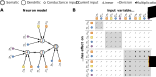
\includegraphics{media/chapters/03_nlif/03_03/nlif_product_terms.pdf}
	\caption[Effects of the relative location of input channels on the dendritic nonlinearity $H$]{Effects of the relative location of input channels on the dendritic nonlinearity $H$. \textbf{(A)}~Dendritic tree used in our example.
	The second compartment is only connected through the soma to the third and fourth compartment.
	\textbf{(B)} Table illustrating how pairs of input channels in \emph{(A)} interact according to \Cref{thm:nlif_product_terms}.
	Grey rectangles correspond to branches with nonlinear interaction.
	The symbol \enquote{$/$} indicates that $H$ only contains linear combinations of terms containing each variable; \enquote{$\div$} indicates that the variable in this column acts divisively on the other variable in the numerator; \enquote{$\bullet$} indicates that $H$ contains product terms with these two variables.}
	\label{fig:nlif_product_terms}
\end{figure}

\begin{definition}[Branch]
A \emph{branch} of an \nlif neuron is a set of compartments that form a connected component in the \nlif connectivity graph even if the somatic compartment is removed from the neuron.
\end{definition}

\begin{restatable}{theorem}{ThmNlifProductTerms}
\label{thm:nlif_product_terms}
Consider an \nlif neuron with $\ell$ branches, where each compartment is connected to $k$ unique con\-duc\-tance- and $k$ unique current-based input channels.
We denote these inputs as $g_j^i$ and $J_j^i$, where $i$ and $j$ are the compartment and input channel indices, respectively.
Furthermore, arrange the compartment indices such that $i_{m - 1} + 1, \ldots, i_{m}$ belong to the same branch, where $m$ with $1 \leq m \leq \ell$ is the branch index.
Then, the somatic current model $H$ has the following form
\begin{align*}
	H_0(g_1^1, \ldots, g_k^1, J_1^1, \ldots, J_k^1) +
	\frac{H^B_1(
		g_1^{2}, \ldots, g_k^{i_1} \!,
		J_1^{2}, \ldots, J_k^{i_1})
	}{
		H^A_1(g_1^{2}, \ldots, g_k^{i_1})
	}
	+ \ldots +
	\frac{H^B_\ell(
		g_1^{i_{\ell - 1} + 1}, \ldots, g_k^{i_\ell},
		J_1^{i_{\ell - 1} + 1}, \ldots, J_k^{i_\ell})
	}{
		H^A_\ell(g_1^{i_{\ell - 1} + 1}, \ldots, g_k^{i_\ell})
	} \,,
%	\label{eqn:nlif_product_terms}
\end{align*}
where \emph{(A)}~$H_0$ is an \emph{affine} function over all inputs injected into the somatic compartment, \emph{(B)}~the $H^A_m$ are nonnegative affine functions of product terms between conductanced-based inputs belonging to \emph{different} dendritic compartments, and \emph{(C)}~the $H^B_m$ are affine functions of product terms between conductance-based inputs belonging to \emph{different} dendritic compartments, and \emph{at most one} dendritic current-based input per product term.
\end{restatable}

\subsubsection{Affine terms}
The \enquote{computationally weakest} \nlif neurons are those where the somatic current is merely an affine function over the input channels.
As follows from \Cref{thm:nlif_product_terms}, this is the case for \nlif neurons that only possess a somatic compartment, or, more generally, any \nlif neuron where input is solely fed into the somatic compartment.
The same holds for \nlif neurons that only possess current-based input channels.

\subsubsection{Shunting}
\Cref{thm:nlif_product_terms} similarly dictates that nonlinear interaction between the input channels of an individual dendritic compartment is limited to \enquote{shunting} \citep[cf.][Section~1.5]{koch1999biophysics}.
That is, conductance-based input channels act \enquote{divisively} on the other input channels in that compartment; they contribute to the denominator of one of the fractions in \Cref{thm:nlif_product_terms}.

Mathematically, this kind of nonlinear interaction is apparent in the dendritic nonlinearity for the two-compartment neuron (eq.~\ref{eqn:two_comp_lif}); the excitatory and inhibitory conductances $g_\mathrm{E}$ and $g_\mathrm{I}$ act divisively on $H$.
While the magnitude of this effect depends on the ratio between the input and the coupling- and leak-conductances, shunting in a single compartment cannot be used to compute \enquote{interesting} functions such as \XOR (proof in \Cref{app:thm_two_comp_xor}):
\begin{restatable}{theorem}{ThmTwoCompXor}
\label{thm:two_comp_xor}
Let $g_\mathrm{E}(x_1, x_2) = g_\mathrm{E}^1(x_1) + g_\mathrm{E}^2(x_2)$ and $g_\mathrm{I}(x_1, x_2) = g_\mathrm{I}^1(x_1) + g_\mathrm{E}^2(x_2)$ be nonnegative functions.
Furthermore, let $a_0 > 0$ and $a_1, a_2, b_0, b_1, b_2 \geq 0$.
The two-compartment \LIF nonlinearity
\begin{align*}
	\phi(x_1, x_2) = H(g_\mathrm{E}(x_1, x_2), g_\mathrm{I}(x_1, x_2)) &= \frac{b_0 + b_1 g_\mathrm{E}(x_1, x_2) - b_2 g_\mathrm{I}(x_1, x_2)}{a_0 + a_1 g_\mathrm{E}(x_1, x_2) + a_2 g_\mathrm{I}(x_1, x_2)}
\end{align*}
cannot be used to solve the weak \XOR problem (see \Cref{def:weak_xor}).
\end{restatable}

Still, and as we demonstrate in the next section, a single layer of two-compartment neurons can compute a wide range of functions with a substantially smaller error than a single layer, or, in some cases, even two layers of standard \LIF neurons.

\subsubsection{Product terms}
Input channels targeting different dendritic compartments interact multiplicatively (cf. eq.~\ref{eqn:three_comp_lif_long}).
%As we discussed above, multiplication over all four quadrants in $[-1, 1]^2$ can be interpreted as a continuous version of the XOR function.
However, exploiting the product terms to compute multiplication over all four quadrants is difficult for multiple reasons.
First, conductance-based inputs are nonnegative, and can thus only cover the quadrant $[0, 1]^2$.
While current-based channels can provide positive and negative input, there is at most one current-based input per product term.

Second, the multiplicative terms are similar in magnitude to the linear terms---for example, all terms in the numerator in \cref{eqn:three_comp_lif_long} are the product of two conductances and one voltage, whereas all terms in the denominator at the product of two conductances.
This implies that, to compute a function such as \XOR, we must find synaptic weights that compensate for the linear terms, while, at the same time, computing the desired nonlinear function.

Lastly, there is a tradeoff between the coupling conductances $c_{ij}$ and the maximum somatic current that can be produced by a compartment.
This current is proportional to the product of the intermediate coupling conductances, making it more difficult for distal compartments to influence the soma.
Countering this by choosing larger $c_{ij}$ results in more linear $H$.

Still, as we demonstrate in \Cref{sec:nlif_opt}, it is indeed possible to solve the weak \XOR problem using a single three-compartment neuron.
In particular, we discuss an iterative weight optimisation scheme that in practice quickly converges to locally optimal weights.


%
%\clearpage
%\setcounter{section}{3}
%% !TeX spellcheck = en_GB

\section{Networks of Two-Compartment LIF Neurons}
\label{sec:two_comp_lif}

Up to this point, we discussed the theoretical advantages of dendritic computation, extended the Neural Engineering Framework to support more complex connectivity constraints and neuron types, and introduced and analysed a family of multi-compartment \LIF neurons with passive dendritic trees that we called \enquote{\nlif} neurons.

The goal of this section is to systematically incorporate the simplest non-trivial \nlif neuron into \NEF networks---namely the two-compartment \LIF neuron depicted in \Cref{fig:nlif_c}.
This represents the smallest possible step toward exploiting dendritic nonlinearities, and as such is a good test for our overall methodology.

We proceed as follows.
First, we discuss a method for estimating the parameters of our surrogate dendritic nonlinearity model $H$ using non-negative least-squares and test the quality of the estimated parameters in various scenarios.
A similar approach can be used derive a \qprog for the synaptic weights that takes nonnegative connectivity and \gls{subrelax} into account.
We use this approach to evaluate the computational advantage of the two-compartment \LIF nonlinearity in an optimal scenario without dynamics, akin to our experiment in \Cref{sec:dendritic_computation_theory_numerical}.
Finally, we demonstrate that this theoretical advantage persists in a spiking neural network context.

\subsection{Estimating Model Parameters}
\label{sec:two_comp_lif_fit_model}

We presented the parametrised dendritic nonlinearity surrogate model for two-compartment \LIF neurons in \cref{eqn:two_comp_lif}.
While the model parameters $a_0$, $a_1$, $a_2$, $b_0$, $b_1$, $b_2$ can be estimated using \cref{eqn:two_comp_lif_natural}, it is better to fit the parameters to data from numerical simulations.

One way to generate these data is to simulate the spiking neuron for different input conductances $g_{\mathrm{E}, k}$, $g_{\mathrm{I}, k}$ over a period of time $T$ and to compute the average spike rate $a_k = \mathscr{G}( g_{\mathrm{E}, k}, g_{\mathrm{I}, k})$.
As discussed in \Cref{sec:nef_nonlinear}, we then obtain the somatic current $J_k$ by applying the inverse of the chosen one-dimensional response curve $G^{-1}$ to $a_k$.
%From our experience, this method yields results superior to measuring $J_k$ directly in the simulation.
Importantly, when doing this, samples with small $a_k$ should be ignored: $G^{-1}$ is not well-defined for zero rates, and $H$ was derived for superthreshold dynamics.

\subsubsection{Optimisation problem}
Given the superthreshold samples $J_k$, $g_{\mathrm{E}, k}$, $g_{\mathrm{I}, k}$ we now have the following least-squares loss function over the parameters $a_i$, $b_i$:
\begin{align}
	E &=
		\sum_{k = 1}^N \bigl( J_k - H(g_\mathrm{E, k}, g_\mathrm{I, k}) \bigr)^2
	= \sum_{k = 1}^N \left( \! J_k - \frac{b_0 + b_1 g_{\mathrm{E}, k} - b_2 g_{\mathrm{E}, k}}{a_0 + a_1 g_{\mathrm{E}, k} + a_2  g_{\mathrm{I}, k}} \right)^2 \,,
	\;\; \begin{aligned}\text{subject to } a_0 &> 0 \,, \\ \text{and } a_1, a_2, b_0, b_1, b_2 &\geq  0 \,.\end{aligned}
	\label{eqn:two_comp_optimal_parameters}
\end{align}
Note that this optimisation problem has one superfluous degree of freedom.
A numerically stable normalisation is to set $b_1 = 1$.
In this case, all parameters are expressed relative to the effect of the excitatory channel on the input current.%
\footnote{As we mentioned in a footnote above, this is a result of the the scale-invariance of the individual rows of $\mat{\tilde A}$ and $\vec{\tilde b}$. In general, a parameterised \nlif neuron has $n - 1$ superfluous degrees of freedom in its parameters.}

\begin{figure}
	\centering
	\includegraphics{media/chapters/03_nlif/03_04/two_comp_lif_loss_comparison.pdf}
	\caption[Comparison between the actual and substitute loss function.]{Comparison between the actual loss function (eq.~\ref{eqn:two_comp_optimal_parameters}; \textbf{A}) and the substitute loss function (eq.~\ref{eqn:two_comp_optimal_parameters_prime}; \textbf{B}).
	Each plot depicts a slice of the error function $E$ or $E'$ over two parameters.
	Black crosses correspond to the optimal solution with respect to the substitute loss function $E'$, black circles correspond to the closest local optimum in the actual loss function.
	The underlying data is sampled from a \gls{twocomp} with  $E_\mathrm{E} = \SI{20}{\milli\volt}$, $E_\mathrm{I} = \SI{-75}{\milli\volt}$, $E_\mathrm{L} = \SI{-65}{\milli\volt}$, $g_\mathrm{L} = \SI{50}{\nano\siemens}$, $c_{12} =\SI{30}{\nano\siemens}$ for $N = 318$ superthreshold samples of $\gE$, $\gI$ over $[\SI{0}{\nano\siemens}, \SI{500}{\nano\siemens}]$.
	The \RMSE current error for the optimised weights is $\sqrt{E/N} = \SI{15.22}{\pico\ampere}$ when using the actual loss function for optimisation, and $\sqrt{E/N} = \SI{15.67}{\pico\ampere}$ when using the substitute loss function for optimisation ($3\%$ increase). The parameter $b_1$ is set to one.
	}
	\label{fig:two_comp_lif_loss_comparison}
\end{figure}

Unfortunately, \cref{eqn:two_comp_optimal_parameters} is neither in \emph{linear} least-squares form, nor convex.
%(see \Cref{app:two_comp_lif_non_convex}).
In theory, this complicates solving for model parameters \citep{rockafellar1993lagrange}.
Fortunately, we can largely work around this by minimising a convex substitute loss function (cf.~\Cref{fig:two_comp_lif_loss_comparison}).
Optimally, we would like the following equality to hold for each sample $k$
\begin{align*}
	J_k &= H(g_{\mathrm{E}, k}, g_{\mathrm{I}, k}) = \frac{
		b_0 + b_1 g_{\mathrm{E}, k} - b_2 g_{\mathrm{I}, k}
	}{
		a_0 + a_1 g_{\mathrm{E}, k} + a_2 g_{\mathrm{I}, k}
 	} \Leftrightarrow 0 = J_k (a_0 + a_1 g_{\mathrm{E}, k} + a_2 g_{\mathrm{I}, k}) - b_0 - b_1 g_{\mathrm{E}, k} + b_2 g_{\mathrm{I}, k} \,.
\end{align*}
Notably, the two equations are equivalent because the denominator is strictly non-zero.
Phrasing this as a loss function for multiple samples yields
\begin{align}
	E' &= \sum_{k = 1}^N \bigl( J_k (a_0 + a_1 g_{\mathrm{E}, k} + a_2 g_{\mathrm{I}, k}) - b_0 - b_1 g_{\mathrm{E}, k} + b_2 g_{\mathrm{I}, k} \bigr)^2 \,,
	\label{eqn:two_comp_optimal_parameters_prime}
\end{align}
subject to the same constraints as above.
Arranging the samples in vectors $\vec J$, $\vec g_\mathrm{E}$, $\vec g_\mathrm{I} \in \mathbb{R}^N$, we can bring this into a canonical matrix form (where \enquote{$\circ$} is elementwise multiplication):
\begin{align}
	E' &= \|\mat A \vec \omega - \vec b \|_2^2 \,, & \text{where } \mat A = (\vec J, \vec J \, \circ \,  \vec g_\mathrm{E}, \vec J \, \circ \, \vec g_\mathrm{I}, -\vec{1}, \vec{g}_\mathrm{I}) \,, \; \vec b = \vec{g}_\mathrm{E} \,, \; \vec \omega &= (a_0, a_1, a_2, b_0, b_2) \,.
	\label{eqn:two_comp_optimal_parameters_prime_matrix}
\end{align}

Crucially, and as is illustrated in \Cref{fig:two_comp_lif_loss_comparison}, the solutions obtained by minimising \cref{eqn:two_comp_optimal_parameters,eqn:two_comp_optimal_parameters_prime} are similar, but not equivalent.
While both optimisation problems minimise the error for each sample, multiplication with the denominator in \cref{eqn:two_comp_optimal_parameters_prime} causes samples to be dynamically re-weighted.
In our application, the impact of this is fairly low in practice, and the global minimum of the substitute loss seems to be close to a minimum in the actual loss function.
This method has been proposed in the context of fitting transfer functions by \citet{levy1959complexcurve}.

\subsubsection{Parameter refinement}
If an exact solution in terms of the closest local optimum of \cref{eqn:two_comp_optimal_parameters} is desired, the parameters can easily be refined using gradient descent.
Alternatively, and as originally suggested by \citet{sanathanan1963transfer} in the context of fitting transfer functions, we can refine the solution by iterative reweighting of \cref{eqn:two_comp_optimal_parameters_prime_matrix}.
Each sample is weighted by the inverse of its denominator from the previous iteration, i.e.,
\begin{align}
	E' &= \|\diag(\vec w)^{-1} \mat A \vec \omega - \diag(\vec w)^{-1}\vec b \|_2^2 \,, & \text{where } \vec w = a_0 \vec{1} + a_1 \vec g_\mathrm{E} + a_2 \vec g_\mathrm{I} \,.
	\label{eqn:sanathanan_koerner}
\end{align}
This scheme converges to a (not necessarily globally optimal) fixed point.
In our application this seems to be the case after two additional iterations.
A more thorough review of this \enquote{Sanathanan-Koerner iteration} is given in \citet[Section~2.2]{hokanson2018least} and \citet{pintelon1994parametric}.
For the sake of simplicity, and because we do not observe a significant reduction in errors, we chose not to rely on this parameter refinement in our experiments.

\subsection{Experiment 1: Precision of the Model Parameter Estimation}
\label{sec:two_comp_lif_experiment_1}

The following experiment tests in how far the surrogate model $G[H(\gE, \gI)]$ can be used to accurately predict the spike rate $\mathscr{G}(\gE, \gI)$ of a simulated spiking two-compartment \LIF neuron---both before and after fitting the model parameters to empirical data.
We conduct this experiment in an artificial scenario with constant conductances \gE, \gI, and in a simulated network context with artificial temporal spike noise superimposed onto the inputs.

\begin{figure}[t]
	\includegraphics{media/chapters/03_nlif/03_04/model_parameter_fits_a.pdf}%
	{\phantomsubcaption\label{fig:synaptic_nonlinearity_fit_a_a}}%
	{\phantomsubcaption\label{fig:synaptic_nonlinearity_fit_a_b}}%
	\caption[Two-compartment nonlinearity model for constant input]{
		Two-compartment nonlinearity model for constant input. Contour plots depict measured average spike rates $\mathscr{G}(g_\mathrm{E}, g_\mathrm{I})$.
		Dashed lines are the model prediction $G[H(g_\mathrm{E}, g_\mathrm{I})]$. Dotted lines indicate the cross-section location.
		$E$ denotes the spike-rate \RMSE.
		Columns correspond to different coupling conductances $c_\mathrm{12}$.
		The model fits the simulation well, with minor deviations near the spike onset.}
	\label{fig:synaptic_nonlinearity_fit_a}%
\end{figure}

\subsubsection{Experiment 1.1: Constant conductances}
We analyse three two-compartment \LIF neurons with coupling conductances $c_{12} = \SI{50}{\nano\siemens}$, $\SI{100}{\nano\siemens}$, and $\SI{200}{\nano\siemens}$; all other parameters are listed in \Cref{tbl:two_comp_neuron_parameters}.
We measure the output spike rate for constant input conductances $g_\mathrm{E}$, $g_\mathrm{I}$ on a $100 \times 100$ grid.
For each grid-point, the neuron's dynamical system (cf.~\Cref{sec:nlif_description}) is simulated for $T = \SI{1}{\second}$.
We then compute the steady-state firing rate by taking the inverse of the median inter-spike-interval.
The conductance range has been selected such that the maximum rate is \SI{100}{\per\second}, and the spike onset coincides with the diagonal of the \gE-\gI-rate contour plot.

We compare these numerical simulation results to both the theoretical somatic current prediction according to \cref{eqn:two_comp_lif_natural}, and the parameterised dendritic nonlinearity with the parameters fitted to the measured data.
Parameter optimisation according to \cref{eqn:two_comp_optimal_parameters_prime_matrix} is based on a training-set of \num{200} conductance pairs sampled with uniform probability from the conductance-range.
The final prediction error is computed over all \num{10000} grid points.

\pagebreak

\paragraph{Results}
The results for this experiment are depicted in \Cref{fig:synaptic_nonlinearity_fit_a}; the fitted parameters can be found in \Cref{tbl:two_comp_model_parameters}.
Unsurprisingly, when using the theoretical parameter estimate from \cref{eqn:two_comp_lif_natural}, there is a substantial discrepancy between the model prediction and the simulation, especially for large $c_{12}$ (\Cref{fig:synaptic_nonlinearity_fit_a_a}). This discrepancy is reduced after fitting the model parameters (\Cref{fig:synaptic_nonlinearity_fit_a_b}).
The model prediction fits the empirical data well for output spike rates greater than \SI{25}{\per\second}.
However, it fails to predict the spike onset correctly, placing it too early with respect to increasing \gE.
As we predicted in \Cref{sec:nlif_theory}, the linearity of $H$ increases as $c_{12}$ is increased, i.e., the contour lines become more \enquote{parallel} for larger $c_{12}$.

\paragraph{Discussion}
Overall, the model works well once the parameters have been fitted.
The mismatch between measured rates and the theoretical model for large $c_{12}$ is likely due to the more pronounced effect of the somatic superthreshold dynamics on the dendritic compartment.
Failure to predict the spike onset is likely due to our model not capturing low firing-rate regimes of the neuron well.

\subsubsection{Experiment 1.2: Conductances with artificial temporal spike noise}

\begin{figure}[t]
	\includegraphics{media/chapters/03_nlif/03_04/model_parameter_fits_b.pdf}%
	\caption[Two-compartment nonlinearity model for noisy input]{Two-compartment nonlinearity model for noisy input with combined excitatory Poisson spike rates of $1/\lambda = \SI{4500}{\per\second}$ for excitatory synapses and $1/\lambda = \SI{1800}{\per\second}$ for inhibitory synapses.
	See \Cref{fig:synaptic_nonlinearity_fit_a} for a complete legend.
	The model fits the noisy data better than the noise-free data.
	    }
	\label{fig:synaptic_nonlinearity_fit_b}%
\end{figure}

In a network context, \gE and \gI are not constant, but, as we discussed in Section~2.2.2, a weighted sum of low-pass filtered spike trains.
This results in a considerable amount of \enquote{spike noise} in the conductance inputs.
In this experiment, we generate artificial filtered spike trains using spike times from Poisson sources (simulation period $T = \SI{100}{\second}$; rates fitted to data from Experiment~3; see below).
Synaptic weights are simulated by uniformly sampling scaling factors for each spike event.
The resulting signals are scaled such that the averages conductances are equal to \gE, \gI.
We de
We furthermore replace $G[J]$ with a ReLU, that is $G[J] = \max\{ 0, \alpha J + \beta \}$.
We know from preliminary experiments that the hard \LIF spike-onset is not present in noisy environments---this is not captured well by the standard \LIF response curve.
While we could use a \enquote{soft} version of the \LIF response curve that takes this into account \citep[cf.][]{capocelli1971diffusion,hunsberger2014competing,kreutz2015mean}, a \ReLU appears to work well.

\paragraph{Results}
The results of this experiment are depicted in \Cref{fig:synaptic_nonlinearity_fit_b}.
Final fitted parameters are provided in \Cref{tbl:two_comp_model_parameters}.
Surprisingly, our model fits the noisy spike rates better than non-noisy data.
Still, the overall trends from the previous experiment are still visible.
When using the theoretical parameter estimates, larger $c_{12}$ result in higher overall errors and fitting the model parameters greatly reduces the error to values of about \SIrange{1}{2}{\per\second}.
While the sharp spike onset is no longer present, the model does not capture the subtle sigmoid shape of the response curve near the spike onset that is particularly pronounced for larger $g_\mathrm{C}$.

\paragraph{Discussion}
To summarise, our results indicate that, after fitting the model parameters, the surrogate model $H$ can indeed be used to predict the neural response curve $\mathscr{G}(\gE, \gI)$ with a relatively high accuracy in both tested scenarios.
It seems reasonable to choose a different one-dimensional neural response curve $G[J]$ when taking noise in the input into account.


\subsection{Solving for Synaptic Weights}
\label{sec:two_comp_synaptic_weights}

We demonstrated that the surrogate model $H(\gE, \gI)$ can be used to quite accurately predict the firing rates of individual \glspl{twocomp}.
Now, to construct \NEF networks, we must find weights $\vec w^\mathrm{E}_i$, $\vec w^\mathrm{I}_i$ that fulfil the normative tuning-curve constraint from \cref{eqn:dendritic}.

\subsubsection{Optimisation problem}
Given a function $f(\vec x)$ that we would like to compute, we optimally minimise the following least-squares loss over $\vec w^\mathrm{E}_i$, $\vec w^\mathrm{I}_i$ for each post-neuron $i$
\begin{align}
	E &= \frac{1}{\Xrepr} \int_{\Xrepr} \mathcal{E} \left( J_i(f(\vec x)), \frac{
		b_0 + b_1 \langle \vec w^\mathrm{E}_i, \vec a(\vec x) \rangle - b_2 \langle \vec w^\mathrm{I}_i, \vec a(\vec x) \rangle
	}{
		a_0 + a_1 \langle \vec w^\mathrm{E}_i, \vec a(\vec x) \rangle + a_2 \langle \vec w^\mathrm{I}_i, \vec a(\vec x) \rangle
 	}	
	\right)^2 \, d\vec x + \sigma^2 \| \vec w^\mathrm{E}_i \|^2_2 + \sigma^2 \| \vec w^\mathrm{I}_i \|^2_2 \,,
	\label{eqn:two_comp_optimal_weights}
\end{align}
subject to $\vec w^\mathrm{E}_i$, $\vec w^\mathrm{I}_i \geq 0$,
and where $\mathcal{E}$ is the superthreshold error function (eq.~\ref{eqn:subthreshold_error}), $\vec a(\vec x)$ are the stacked pre-activities of all pre-populations, and $J_i(\vec x)$ is the current-translation function.

Just like the model parameter optimisation problem from the previous subsection, \cref{eqn:two_comp_optimal_weights} is not convex.
%(again, see \Cref{app:two_comp_lif_non_convex} for more details).
Again, we work around this by multiplying with the denominator inside the square to obtain a substitute loss function:
\begin{align}
	\begin{aligned}
	E' &=
		\int_{\Xrepr} \mathcal{E}
		\Bigl(
			J_i(f(\vec x)) (a_0 + a_1 \langle \vec w^\mathrm{E}_i, \vec a(\vec x) \rangle + a_2 \langle \vec w^\mathrm{I}_i, \vec a(\vec x) \rangle )\,, \\[-1em]
		&\hspace{3.66em}		
		b_0 + b_1 \langle \vec w^\mathrm{E}_i, \vec a(\vec x) \rangle - b_2 \langle \vec w^\mathrm{I}_i, \vec a(\vec x) \rangle
		\Bigr)^2 \, d\vec x
		 + \sigma^2 \| \vec w^\mathrm{E}_i \|^2_2 + \sigma^2 \| \vec w^\mathrm{I}_i \|^2_2 \,,
	\end{aligned}
	\label{eqn:two_comp_optimal_weights_prime}
\end{align}
subject to $\vec w^\mathrm{E}_i$, $\vec w^\mathrm{I}_i \geq 0$.
A sampled version of this problem can be phrased as a \qprog.
To see this, let $\mat A \in \mathbb{R}^{N \times n}$ be a matrix of pre-activities and $\vec J_i \in \mathbb{R}^{N}$ be a vector of target currents.
Assume that we only have superthreshold samples, that is $\mathcal{E}(J_\mathrm{tar}, J_\mathrm{dec}) = J_\mathrm{tar} - J_\mathrm{dec}$. We have:
\begin{align}
	E' &\propto \bigl\|	\,
		  \vec J_i \circ
		  	\bigl(
		  		a_0 +
		  		a_1 \mat{A} \vec w_i^\mathrm{E} +
		  		a_2 \mat{A} \vec w_i^\mathrm{E} \bigr)
	      - \bigl(
	      		b_0 +
	      		b_1 \mat{A} \vec w_i^\mathrm{E} -
	      		b_2 \mat{A} \vec w_i^\mathrm{I} \bigr)
	\, \bigr\|_2^2
	+ \sigma^2 \bigl\| \vec w^\mathrm{E}_i \bigr\|^2_2 + \sigma^2 \bigl\| \vec w^\mathrm{I}_i \bigr\|^2_2 \notag \\
		&= \hspace{0.125em} \bigl\|
			\bigl(a_1 \diag(\vec J_i) \mat A - b_1 \mat A \bigr) \vec w_i^\mathrm{E}
			+ \bigl(a_2 \diag(\vec J_i) \mat A + b_2 \mat A \bigr) \vec w_i^\mathrm{I}
			+ (a_0 - b_0) \vec J_i
	\, \bigr\|_2^2
	+ \sigma^2 \bigl\| \vec w^\mathrm{E}_i \bigr\|^2_2 
	+ \sigma^2 \bigl\| \vec w^\mathrm{I}_i \bigr\|^2_2  \notag \\
	&= \hspace{0.125em} \bigl\|
		\mat A' \vec w_i + \vec J_i'
	\bigr\|_2^2
	+ \sigma^2 \bigl\| \vec w_i \bigr\|^2_2  \,.
	\label{eqn:two_comp_optimal_weights_prime_matrix}
\end{align}
To account for \gls{subrelax}, we simply split $\mat A'$ and $\vec J'$ into super- and subthreshold samples as discussed in \Cref{sec:nef_subthreshold} and use the QP defined in \cref{eqn:decode_subthreshold_qp}.

Again, we could use the Sanathanan-Koerner iteration (cf.~eq.~\ref{eqn:sanathanan_koerner}) to refine the solution.
However, in our experience, and as with the parameter optimisation problem, the solution to the convex problem tends to be close to a local optimum in the original rational loss function.

\subsubsection{Examples: Addition and gain modulation}
Although we analyse two-compartment neurons more thoroughly in the next two sections, we would first like to test our weight optimisation scheme in the context of two specific functions $f$: addition and nonnegative multiplication.

Specifically, we use the two-compartment \LIF neuron with $c_{12} = \SI{50}{\nano\siemens}$ (parameter set (ii) from \Cref{tbl:two_comp_neuron_parameters})
and the network setup discussed in
\Cref{sec:dendritic_computation_theory_dendritic}.
That is, two pre-populations with 200 neurons each project onto a single post-neuron; the pre-populations represent $x_1$, $x_2$, respectively, while the post-neuron represents $\hat y \approx f(x_1, x_2)$.%
\footnote{While an individual neuron is not sufficient for reconstructing the represented value $\hat y$ via linear decoding, we can infer $\hat y$ by inverting the current translation function; that is $\hat y = J^{-1}[H(\gE(x_1) + \gE(x_2), \gI(x_1) + \gI(x_2))]$.
Our post-neuron has a positive encoder, an $x$-intercept of zero, and a maximum rate of \SI{100}{\per\second}.
}
As depicted in \Cref{fig:nef_multivariate_functions_c}, the synaptic weights implicitly define a set of conductance functions.
Due to commutativity of addition and multiplication, the excitatory and inhibitory functions decoded from each pre-population optimally are the same; we have $\gE(x) = g_\mathrm{E}^1(x) = g_\mathrm{E}^2(x)$ and $\gI(x) = g_\mathrm{I}^1(x) = g_\mathrm{I}^2(x)$.
We emulate current-based \LIF neurons by setting $a_0 = b_1 = 1$, $b_2 = -1$, and $a_1 = a_2 = b_0 = 0$ in the nonlinearity model $H$.
For these parameters we have $H(J_\mathrm{E}, J_\mathrm{I}) = J_\mathrm{E} - J_\mathrm{I}$.
%while the synaptic weights implicitly describe excitatory and inhibitory current functions $J_\mathrm{E}(x)$ and $J_\mathrm{I}(x)$.

\begin{figure}
	\centering
	\includegraphics{media/chapters/03_nlif/03_04/two_comp_weights_examples_addition.pdf}%
	{\phantomsubcaption\label{fig:two_comp_weights_examples_addition_a}}%
	{\phantomsubcaption\label{fig:two_comp_weights_examples_addition_b}}%
	\caption[Computing addition in single- and \glspl{twocomp}]{Computing addition in \textbf{(A)} single- and \textbf{(B)} \glspl{twocomp}. See text for a detailed description. \emph{Top:} Decoded current and conductance functions. \emph{Left:} Decoded represented value. Black contour lines and coloured backdrop correspond to the decoded values $\hat y$; dashed white lines to the target function $y$. \emph{Right:} Decoding error $\hat y - y$. Depicted error value $E$ is the \NRMSE.
	Single- and \glspl{twocomp} are equally suitable for computing linear functions.
	}
	\label{fig:two_comp_weights_examples_addition}
\end{figure}

%\paragraph{Results: Addition}
Results for computing addition, that is $f(x_1, x_2) = \frac{1}2 (x_1 + x_2)$ over $(x_1, x_2) \in [0, 1]^2$, are depicted in \Cref{fig:two_comp_weights_examples_addition}.
As is expected, we can compute this function with a low \NRMSE with the current-based nonlinearity.
Perhaps unintuitively, and in spite of the dendritic nonlinearity $H$, we achieve similarly low errors using the two-compartment \LIF neuron.

The way in which the weight solver accomplishes this becomes apparent when considering the decoded current functions \gE and \gI in \Cref{fig:two_comp_weights_examples_addition_b}.
Both $\gE$ and $\gI$ are affine functions with opposing slopes.
Correspondingly, the denominator $a_0 + a_1 \gE + a_2 \gI$ stays approximately constant, while the numerator $b_0 + b_1 \gE - b_2 \gI$ generates the desired target currents.


\begin{figure}
	\centering
	\includegraphics{media/chapters/03_nlif/03_04/two_comp_weights_examples_multiplication.pdf}%
	{\phantomsubcaption\label{fig:two_comp_weights_examples_multiplication_a}}%
	{\phantomsubcaption\label{fig:two_comp_weights_examples_multiplication_b}}%
	\caption[Computing multiplication in single- and \glspl{twocomp}]{Computing multiplication in \textbf{(A)} single- and \textbf{(B)} \glspl{twocomp}. See text for a detailed description and \Cref{fig:two_comp_weights_examples_addition} for a legend. Nonnegative multiplication can be reasonably well approximated using \glspl{twocomp}. Dotted line in \emph{(B)} is a hyperbolic fit.
	}
	\label{fig:two_comp_weights_examples_multiplication}
\end{figure}

%\paragraph{Results: Multiplication}
Results for computing nonnegative multiplication, that is $f(x_1, x_2) = x_1 x_2$ over $(x_1, x_2) \in [0, 1]^2$, are depicted in \Cref{fig:two_comp_weights_examples_multiplication}.
Using current-based \LIF neurons we can, at best, approximate multiplication with a linear function. This results in an \NRMSE of about 25\%.
In contrast, using the two-compartment \LIF nonlinearity results in an error of about 6\%, with the largest discrepancies being in regions are both $x_1$ and $x_2$ are close to one.


\begin{figure}
	\centering
	\includegraphics{media/chapters/03_nlif/03_04/two_comp_weights_examples_statistics.pdf}%
	{\phantomsubcaption\label{fig:two_comp_weights_examples_statistics_a}}%
	{\phantomsubcaption\label{fig:two_comp_weights_examples_statistics_b}}%
	{\phantomsubcaption\label{fig:two_comp_weights_examples_statistics_c}}%
	{\phantomsubcaption\label{fig:two_comp_weights_examples_statistics_d}}%
	\caption[Error and weight statistics for computing addition and nonnegative multiplication]{Error and weight statistics for computing addition and nonnegative multiplication. \textbf{(A, B)}
	
	Depicted is the median over $1000$ experiments, shaded areas the 25/75-percentiles.
	While errors monotonically decreases with more pre-neurons in the addition task \emph{(A)}, errors quickly plateau when computing multiplication \emph{(B)}.
	\textbf{(C,~D)}~Comparison between the weight magnitude frequencies for the two tasks and neuron types (for $n = 300$ pre-neurons).
	Weights are normalised such that a value of one corresponds to $\SI{1}{\nano\ampere}$ or $\SI{1}{\nano\siemens}$, respectively.
	Dashed line and depicted values are the median; frequencies include zero-weights. Weights below $10^{-6}$ are counted as zero. \Glspl{twocomp} require larger weight magnitudes. The spread of the magnitudes changes depending on the computed function.
	}
	\label{fig:two_comp_weights_examples_statistics}
\end{figure}

Importantly, and as is depicted in \Cref{fig:two_comp_weights_examples_statistics_b}, two-compartment \LIF neurons cannot approximate nonnegative multiplication with an arbitrarily small error; more precisely, the error cannot be reduced past 6\% for a single post-neuron.
This is in contrast to addition, where we can reach arbitrarily small errors by increasing the number of pre-neurons (cf.~\Cref{fig:two_comp_weights_examples_statistics_a})
It is possible to reach smaller (but not arbitrarily small) errors with multiple post neurons dividing up the represented space (we reach down to $4\%$; see $E_\mathrm{model}$ in \Cref{tbl:function_approximations_complete}).

Curiously, looking at the conductance functions \gE and \gI, \emph{both} excitation and inhibition increase substantially for small $x_1$ or $x_2$, similar to a shifted and scaled hyperbola  $(\beta + \alpha x)^{-1}$ (black dotted line in \Cref{fig:two_comp_weights_examples_multiplication_b}).
This may be counter-intuitive, given that inhibition is typically responsible for shutting off the target neuron.%
\footnote{Remember that these results are for a single post-neuron with positive encoder. That is, to represent smaller values, the neuron must receive a smaller input current.}
However, when increasing both excitation and inhibition, this common-mode increase mostly cancels out in the numerator (due to the inhibitory conductance being subtracted), but increases the magnitude of the denominator; this amplifies the divisive effect of the input.

Notably, as we mentioned in the introduction of this chapter, nonnegative multiplication (or, alternatively, nonnegative division) is also referred to as \enquote{gain modulation} in the neuroscience literature \citep{salinas2000gain}.
The observation that both excitation and inhibition must be increased to multiplicatively (or divisively) reduce the gain of a neuron is consistent with \emph{in vitro} experiments \citep{chance2002gain}.

An earlier hypothesised mechanism for gain modulation is \emph{shunting inhibition}.
Here, the idea is that an inhibitory channel with a reversal potential close to the resting potential acts divisively on the average input current.
This effect could in theory be used to implement multiplication \citep{koch1992multiplying}; however, in practice, increasing inhibitory conductances alone has a predominantly linear effect on the spike rate (since $a_2 \ll b_2$), or requires implausibly high conductance values \citep{holt1997shunting,abbott2005drivers}.

Even when exploiting the common increase of excitation and inhibition, generating the large input conductances for small $x_1$, $x_2$ results in relative large synaptic weights.
This is depicted in \Cref{fig:two_comp_weights_examples_statistics_c,fig:two_comp_weights_examples_statistics_d}.
Compared to computing addition, the median synaptic weight increases by a factor of five.

\subsection{Experiment 2: Theoretical Analysis of Two-Compartment LIF Neurons}
\label{sec:two_comp_lif_experiment_2}

Given the encouraging results from the previous subsection, we would now like to analyse the theoretical advantage of the two-compartment \LIF model in a more systematic manner.
In particular, our goal is to characterise the \enquote{computational power} of different network and neuron types using the methodology from our basis-function experiment in \Cref{sec:dendritic_computation_theory_numerical}.

We implicitly assume that \Hcond accurately describes the somatic current flowing into the \gls{twocomp}.
This is supported by our earlier results from Experiment~1 (\Cref{sec:two_comp_lif_experiment_1}).
Furthermore, note that we abbreviate the \glsdisp{dennonlin}{two-compartment LIF nonlinearity} with conductance-based synapses as \Hcond, and the standard current-based \LIF neuron as \Hcur.
As mentioned before $\Hcur$, is simply defined as $\Hcur(J_\mathrm{E}, J_\mathrm{I}) = J_\mathrm{E} - J_\mathrm{I}$.

\subsubsection{Methods}
Just as in \Cref{sec:dendritic_computation_theory_numerical}, we would like to measure how well different networks can approximate functions of increasing complexity \slc.
We sample random 2D target-current functions $J_\rho$ over $(x_1, x_2) \in [-1, 1]^2$ with an RMS of \SI{0.5}{\nano\ampere} on a $63 \times 63$ grid using the technique illustrated in \Cref{fig:2d_functions_overview}.
We then measure how well $J_\rho$ can be approximated for a single post-neuron given the static tuning of the networks depicted in \Cref{fig:nef_multivariate_functions}.
The pre-populations consist of \num{100} neurons each and project both excitatorily and inhibitorily onto the post-neuron; the intermediate population in the two-layer network (\Cref{fig:nef_multivariate_functions_b}) consists of \num{200} neurons.
In each trial, the pre-population tuning is randomly generated.

All synaptic weights are computed by solving the QP in \cref{eqn:two_comp_optimal_weights_prime_matrix} for 256 randomly selected training samples, with and without \gls{subrelax} (the relaxation threshold is set to \SI{0}{\nano\ampere}).
The regularisation parameters were selected independently for each setup (cf.~\Cref{app:two_comp_regularisation_factor_sweep}).
The final error $E_\mathrm{model}$ is the \NRMSE over all grid points with Gaussian noise (standard deviation $10^{-2} a_\mathrm{max}$) added to the pre-activities to test for generalisation.

\subsubsection{Results}

\begin{figure}
	\centering
	\includegraphics{media/chapters/03_nlif/03_04/two_comp_2d_frequency_sweep.pdf}%
	\kern-158.06mm\includegraphics{media/chapters/03_nlif/03_04/two_comp_2d_frequency_sweep_overlay.pdf}
	\caption[Two-compartment neuron decoding error for random multivariate current functions]{Decoding error for random multivariate current functions.
	\NRMSE between random, two-dimensional current functions and the decoded approximation using different input-dependent nonlinearities; errors are based on the superthreshold error function $\mathcal{E}$ (eq.~\ref{eqn:decode_current_subthreshold}). The low-pass filter coefficient \slc is a proxy for the spatial frequency content in the target function (cf.~\Cref{sec:dendritic_computation_theory_numerical}). All points correspond to the median over \num{100} trials. Dashed lines show results for not taking the \gls{subrelax} into account when solving for weights.
	Dotted lines are theoretical predictions from \Cref{fig:dendritic_computation_fourier_example_b}.	
	The black lines show the results for a linear, current-based \Hcur; blue/green lines show the results for the two-compartment conductance-based model  \Hcond with parameters given in \Cref{tbl:two_comp_model_parameters} (without noise). Orange lines correspond a current-based network with two-dimensional pre-neuron tuning (i.e., a two-layer neural network). Shaded areas correspond to the 25/75 percentile for the current-based models and the conductance-based model with $c_{12} = \SI{50}{\nano\siemens}$.
	}
	\label{fig:two_comp_lif_frequency_sweep}
\end{figure}

Overall, the results depicted in \Cref{fig:two_comp_lif_frequency_sweep} are similar to those from our theoretical basis-function experiment \Cref{sec:nlif_theory} (cf.~\Cref{fig:dendritic_computation_fourier_example}).
In particular, the error curve for the \gls{twocomp} qualitatively resembles the multiplicative nonlinearity, although errors tend to be higher for \Hcond:
the inflection point of the sigmoid is at $\slc \approx 0.7$ for the \twocomplif nonlinearity, and was at $\slc \approx 1$ for the multiplicative nonlinearity.

Similarly to additive network in the basis-function experiment (cf.~the dotted line labelled \enquote{additive baseline}), the median error for \Hcur initially increases almost linearly on a log-log plot, starting from a $2.5\%$ error for low-frequency functions to an error of about $50\%$ for functions with \slc greater than one.
\Gls{subrelax} reduces this error by up to $50\%$.

The error for the conductance-based \twocomplif nonlinearity initially increases sub-linearly on a log-log plot, starting at median errors of about $0.8\%$ for low-frequency functions.
The maximum reduction in the median error compared to the standard-\LIF neuron is about $65\%$.
Errors are competitive with the two-layer network for $\slc < 0.5$.
The error converges to the results for the standard \LIF neuron for $\slc > 1$.
Compared to standard \LIF neurons, the advantage of \gls{subrelax} is, on average, not as pronounced.

\subsubsection{Discussion}
The large errors for \Hcur and \Hcond in regimes with $\slc > 0.5$ are likely due to both functions not being able to solve the \XOR problem (cf.~\Cref{app:thm_two_comp_xor}).
Functions with $\slc \geq 0.5$ may possess multiple maxima/minima over $[-1, 1]^2$ (cf.~\Cref{fig:2d_functions_overview}), akin to \XOR.
Trying to approximate these functions using \Hcur or \Hcond thus leads to a large error.

This observation explains the difference between the multiplicative nonlinearity from the basis-function experiment (see the \enquote{multiplicative baseline} in the above figure) and the two-compartment \LIF neuron---the multiplicative nonlinearity \emph{can} be used to solve the \XOR problem.
Evidently, networks capable of approximating \XOR-like functions are, using our terminology form \Cref{sec:dendritic_computation_theory}, more \enquote{powerful} than those limited to conductance-based shunting.

To summarise, this experiment demonstrates that the \twocomplif \gls{dennonlin} \Hcond substantially reduces the approximation error for $J_\rho$ with $\slc < 1$ compared to an additive network with nonlinearity \Hcur.
The \gls{twocomp} is competitive with a two-layer network for $\slc < 0.5$ and reaches similar errors as the multiplicative nonlinearity.


\subsection{Experiment 3: Dendritic Computation in Spiking Neural Networks}
\label{sec:two_comp_lif_experiment_3}

Our results for Experiment~1 suggest that we can use the \twocomplif nonlinearity \Hcond to predict the average current flowing into the somatic compartment of a \gls{twocomp}.
Furthermore, Experiment~2 shows that we can use \Hcond to approximate a relatively large class of functions well.
In our final experiment, we validate whether these results still hold true in a spiking neural network context.

While we use the same basic network setup as in Experiment~2, we now decode the represented value from a population of \num{100} neurons through time.
Optimally, this decoded value should be $f(x_1, x_2)$, where the input signals $x_1(t), x_2(t) \in [-1, 1]$ are represented by the pre-populations.
Additionally, we now adhere to \gls{dales_principle}.
Neurons are randomly marked as either excitatory or inhibitory, with a 30\% probability of a neuron being inhibitory.

We model fast excitatory synapses as an exponential low-pass (cf.~\Cref{sec:simplified_neuron_models}) with a time-constant of \SI{5}{\milli\second} as observed in glutamatergic pyramidal neurons with AMPA receptor \citep{jonas1993quantal}.
The inhibitory pathway is modeled with a \SI{10}{\milli\second} time-constant as observed in inhibitory interneurons with GABA\textsubscript{A} receptors \citep{gupta2000organizing}.
All remaining neuron parameters can be found in \Cref{tbl:two_comp_neuron_parameters}.


\begin{figure}
	\includegraphics{media/chapters/03_nlif/03_04/two_comp_network_spikes_example.pdf}
	\caption[Computing nonnegative multiplication in a spiking neural network using two-compartment LIF neurons]{Computing nonnegative multiplication in a spiking neural network using two-compartment LIF neurons.
	\textbf{(A)} \emph{Top two plots:} inputs $x_1(t)$ and $x_2(t)$ as represented by the two pre-populations. The input is a fourth order 2D Hilbert curve. \emph{Bottom:} mathematical target $f(x_1(t), x_2(t)) = (x_1(t) + 1) (x_2(t) + 1) / 4$, filtered target function, as well as the decoded target population output.
	\textbf{(B)} Spike raster plots corresponding to the spiking activity of each of the populations (only half of the neurons are depicted). Red shaded background corresponds to inhibitory neurons in the pre-populations, all other neurons are excitatory.}
	\label{fig:two_comp_lif_spiking_example}
\end{figure}

In each trial, we simulate the network over \SI{10}{\second} at a time-resolution of \SI{100}{\micro\second}.
Inputs $x_1(t)$ and $x_2(t)$ are moving along a fourth-order space-filling Hilbert curve\index{Hilbert curve} covering $[-1, 1]^2$ \citep{hilbert1891uber}.
The activities of the output population are decoded and filtered with a first-order exponential low-pass at $\tau = \SI{100}{\milli\second}$.
To determine the approximation error, we pass the target $f(x_1(t), x_2(t))$ through exactly the same filter chain.
Our final error $E_\mathrm{net}$ is the \NRMSE between the decoded output and the filtered target signal over time.
\Cref{fig:two_comp_lif_spiking_example} depicts a single trial.

Again, all synaptic weights are computed by solving the \QP in \cref{eqn:two_comp_optimal_weights_prime_matrix}.
We set the relaxation threshold for \gls{subrelax} to $75\%$ of $J_\mathrm{th}$, as suggested by our experiments in \Cref{sec:nef_subthreshold}.
The regularisation factor $\sigma$ has been selected independently for each parameter set such that $E_\mathrm{net}$ is minimised when computing nonnegative multiplication (cf.~\Cref{app:two_comp_regularisation_factor_sweep}).

\subsubsection{Experiment 3.1: Random bandlimited functions}

\begin{figure}[t]
	\centering
	{\includegraphics{media/chapters/03_nlif/03_04/two_comp_2d_frequency_sweep_network.pdf}}%
	\kern-158.06mm\includegraphics{media/chapters/03_nlif/03_04/two_comp_2d_frequency_sweep_overlay.pdf}
	\caption[Median error for computing random bandlimited functions in a feed-forward network over 100 trials]{Median error for computing random bandlimited functions in a feed-forward network over 100 trials. Measured \NRMSE is the difference between the represented value $\hat y(t)$ and the expected value $f_\rho(x_1(t), x_2(t))$ relative to the standard deviation of $f_\rho$. See \Cref{fig:two_comp_lif_frequency_sweep} for a more detailed description.}
	\label{fig:frequency_sweep_network}
\end{figure}

We first test our setup with the bandlimited functions $f_\rho$ used in Experiment~2.
Results are depicted in \Cref{fig:frequency_sweep_network}.
Qualitatively, the results are similar to what we saw before, although the minimum errors are substantially higher.
The reduction in error between the current- and conductance-based models is not quite as large as suggested by the previous experiment, with a maximum reduction (in terms of the median) of only $40\%$ (instead of $65\%$ before).
While \gls{subrelax} mostly increases the performance of the current-based model in the previous experiment, the improvement in error is now clearly visible for the conductance-based model as well (especially for $c_{12} = \SI{50}{\nano\siemens}$).

Notably, the minimum median approximation error of the two-layer network is about $10\%$, whereas the single-layer current- and conductance-based models reach minimum errors of about $6\%$ and $4\%$, respectively. The two-layer network clearly surpasses the performance of the two-compartment \LIF single-layer network for $\slc > 0.6$.

\paragraph{Discussion}

The elevated error levels are likely due to the spike noise that is now superimposed onto all input signals.
Notably, this noise, as well as the added dynamics, do not affect the \glspl{twocomp} over-proportionally, as one might expect due to the simplifications made during the derivation of the \glsdisp{dennonlin}{dendritic nonlinearity model} (cf.~\Cref{sec:nlif_derive_h}).
To the contrary, the largest effect of the additional noise is on the two-layer network.

We think that the larger errors for the two-layer network are caused by the representation of a two-dimensional quantity begin noisier than the representation of the individual scalars in the two pre-populations.
This is in line with our observation from \Cref{sec:dendritic_computation_theory_numerical}.
Given a maximum error, the number of basis functions decodable from a multi-dimensional population is not much larger than the decodable function count for a one-dimensional population.

To solve this issue, we would optimally have to square the number of neurons used in the intermediate layer.
In our case, we would have to use $100^2 = \num{10000}$ instead of \num{200}, which would not really be comparable to the single-layer setups.

\subsubsection{Experiment 3.2: Benchmark functions}

\begin{table}[t]
	\caption[Spiking neural network approximation errors.]{Spiking neural network approximation errors for function approximations on $[0, 1]^2$. Error values correspond to the \NRMSE and are measured as the difference between the output decoded from the target population and the desired output for a ten second sweep across a 4th order 2D Hilbert curve\index{Hilbert curve} over the input space. Results are the mean and standard deviation over 256 trials. The best result for a target function is set in bold; darker background colours indicate a worse ranking of the result in the corresponding row. Columns labeled \enquote{standard} refer to the default, single layer network setup, \enquote{two layers} refers to the two-layer setup, and \enquote{noisy} to the single layer network setup with model parameters derived under noise (see Experiment 1.2). Additional tables can be found in \Cref{app:data_chp3}.}
	\fontsize{10pt}{12pt}\selectfont
	\renewcommand\arraystretch{1.2}
	\sffamily
	%--------------------------------------------
	\begin{tabular}{r r r r r r r r }
	\toprule
	\textbf{Target}& \multicolumn{7}{c}{\textbf{Experiment setup}} \\
	\cmidrule(r){1-1}\cmidrule(l){2-8}
	& \multicolumn{3}{c}{%0
	LIF}
	& \multicolumn{2}{c}{%1
	Two comp. $c_{12} = \SI{50}{\nano\siemens}$}
	& \multicolumn{2}{c}{%2
	Two comp. $c_{12} = \SI{100}{\nano\siemens}$}
	\\
	\cmidrule(l){2-4}
	\cmidrule(l){5-6}
	\cmidrule(l){7-8}
	& standard
	& standard\textsuperscript{\dag}
	& two layers\textsuperscript{\dag}
	& %0
	standard\textsuperscript{\dag}
	& %1
	noisy\textsuperscript{\dag}
	& %0
	standard\textsuperscript{\dag}
	& %1
	noisy\textsuperscript{\dag}
	\\
	\midrule
	$x_1 + x_2$ 
	& \cellcolor{White!72!SteelBlue}$5.7 \pm 0.2\%$
	& \cellcolor{White!58!SteelBlue}$5.8 \pm 0.3\%$
	& \cellcolor{White!29!SteelBlue}$9.9 \pm 0.4\%$
	& \cellcolor{White!100!SteelBlue}$\mathbf{4.3 \pm 0.3\%}$
	& \cellcolor{White!43!SteelBlue}$8.2 \pm 0.9\%$
	& \cellcolor{White!86!SteelBlue}$4.7 \pm 0.3\%$
	& \cellcolor{White!15!SteelBlue}$11.2 \pm 0.9\%$
	\\
	$x_1 \times x_2$ 
	& \cellcolor{White!15!SteelBlue}$25.8 \pm 1.2\%$
	& \cellcolor{White!29!SteelBlue}$15.5 \pm 1.2\%$
	& \cellcolor{White!43!SteelBlue}$9.2 \pm 0.3\%$
	& \cellcolor{White!100!SteelBlue}$\mathbf{4.4 \pm 0.6\%}$
	& \cellcolor{White!86!SteelBlue}$4.7 \pm 0.4\%$
	& \cellcolor{White!72!SteelBlue}$5.4 \pm 0.6\%$
	& \cellcolor{White!58!SteelBlue}$6.9 \pm 0.4\%$
	\\
	$\sqrt{x_1 \times x_2}$ 
	& \cellcolor{White!15!SteelBlue}$24.9 \pm 1.8\%$
	& \cellcolor{White!29!SteelBlue}$14.7 \pm 1.7\%$
	& \cellcolor{White!43!SteelBlue}$12.6 \pm 0.9\%$
	& \cellcolor{White!86!SteelBlue}$7.1 \pm 0.9\%$
	& \cellcolor{White!100!SteelBlue}$\mathbf{6.0 \pm 0.7\%}$
	& \cellcolor{White!58!SteelBlue}$7.7 \pm 1.0\%$
	& \cellcolor{White!72!SteelBlue}$7.6 \pm 0.6\%$
	\\
	$(x_1 \times x_2) ^ 2$ 
	& \cellcolor{White!15!SteelBlue}$23.1 \pm 0.7\%$
	& \cellcolor{White!29!SteelBlue}$16.2 \pm 0.9\%$
	& \cellcolor{White!43!SteelBlue}$9.3 \pm 0.5\%$
	& \cellcolor{White!86!SteelBlue}$5.1 \pm 0.9\%$
	& \cellcolor{White!100!SteelBlue}$\mathbf{3.9 \pm 0.6\%}$
	& \cellcolor{White!72!SteelBlue}$7.2 \pm 1.2\%$
	& \cellcolor{White!58!SteelBlue}$8.8 \pm 1.0\%$
	\\
	$x_1 / (1 + x_2)$ 
	& \cellcolor{White!15!SteelBlue}$15.0 \pm 0.7\%$
	& \cellcolor{White!58!SteelBlue}$10.1 \pm 0.8\%$
	& \cellcolor{White!72!SteelBlue}$9.2 \pm 0.6\%$
	& \cellcolor{White!100!SteelBlue}$\mathbf{4.5 \pm 0.4\%}$
	& \cellcolor{White!43!SteelBlue}$11.4 \pm 1.7\%$
	& \cellcolor{White!86!SteelBlue}$6.1 \pm 0.6\%$
	& \cellcolor{White!29!SteelBlue}$14.8 \pm 1.8\%$
	\\
	$\|(x_1, x_2)\|$ 
	& \cellcolor{White!15!SteelBlue}$18.6 \pm 0.6\%$
	& \cellcolor{White!43!SteelBlue}$10.8 \pm 0.9\%$
	& \cellcolor{White!58!SteelBlue}$9.7 \pm 0.4\%$
	& \cellcolor{White!100!SteelBlue}$\mathbf{5.3 \pm 0.5\%}$
	& \cellcolor{White!72!SteelBlue}$8.2 \pm 0.9\%$
	& \cellcolor{White!86!SteelBlue}$6.0 \pm 0.6\%$
	& \cellcolor{White!29!SteelBlue}$12.1 \pm 0.9\%$
	\\
	$\mathrm{atan}(x_1, x_2)$ 
	& \cellcolor{White!15!SteelBlue}$17.8 \pm 1.0\%$
	& \cellcolor{White!43!SteelBlue}$12.4 \pm 1.0\%$
	& \cellcolor{White!29!SteelBlue}$12.5 \pm 0.8\%$
	& \cellcolor{White!100!SteelBlue}$\mathbf{7.2 \pm 1.8\%}$
	& \cellcolor{White!86!SteelBlue}$7.5 \pm 1.5\%$
	& \cellcolor{White!58!SteelBlue}$8.3 \pm 1.8\%$
	& \cellcolor{White!72!SteelBlue}$8.1 \pm 1.0\%$
	\\
	$\max(x_1, x_2)$ 
	& \cellcolor{White!15!SteelBlue}$34.5 \pm 1.1\%$
	& \cellcolor{White!29!SteelBlue}$22.6 \pm 1.4\%$
	& \cellcolor{White!86!SteelBlue}$10.0 \pm 0.4\%$
	& \cellcolor{White!72!SteelBlue}$12.9 \pm 1.5\%$
	& \cellcolor{White!100!SteelBlue}$\mathbf{9.9 \pm 1.3\%}$
	& \cellcolor{White!58!SteelBlue}$14.9 \pm 1.8\%$
	& \cellcolor{White!43!SteelBlue}$16.3 \pm 0.9\%$
	\\
	\bottomrule
	\end{tabular}\\[0.25cm]
	%--------------------------------------------
	\raggedright\textsuperscript{\dag}With \gls{subrelax}
	\label{tbl:function_approximations}
\end{table}

While the random functions in the above experiments are useful to systematically characterise the individual setups, it is hard to tell from these data alone what the impact of using \glspl{twocomp} could be in practice.
To this end, we selected eight benchmark functions $f(x_1, x_2)$ typically found in models of neurobiological systems and repeated the experiment.
See \Cref{tbl:two_comp_functions} for a detailed list.

Note that we rescale the input such that $(x_1, x_2) \in [-1, 1]^2$ map onto $[0, 1]^2$ and $[-1, 1]$.
Similarly, we rescale the output of each function to fully cover the codomain $[-1, 1]$.
This ensures that we fully utilise the range of values that can be represented by the neuron populations, while restricting functions such as multiplication to a single quadrant.

\paragraph{Results}
A summary of the results over $256$ trials per function and setup is given in \Cref{tbl:function_approximations}.
More detailed results can be found in \Cref{tbl:function_approximations_complete}.
The \glsdisp{twocomp}{two-compartment model} with a coupling conductance of $g_\mathrm{C} = \SI{50}{\nano\second}$ achieves the smallest error $E_\mathrm{net}$ across all target functions.

Using the \gls{dennonlin} model parameters derived under noise (cf.~\Cref{sec:two_comp_lif_experiment_1}) is beneficial when computing multiplicative functions and the maximum.
For these target functions, the synaptic connection matrix tends to be sparser, increasing individual parameter weights and thus input noise (cf.~\Cref{fig:two_comp_weights_examples_statistics_c,fig:two_comp_weights_examples_statistics_d}).
%This increase in noise matches the environment the neuron parameters have been optimised for.

The minimum error for the two-layer network is about $9\%$ even for simple functions, matching the observation we made in the random function experiment above.
The current-based neuron is only competetive with the \gls{twocomp} for computing addition.
\Gls{subrelax} decreases the error by up to $40\%$.

\paragraph{Discussion}
An effect that could contribute to the superior performance of the \gls{twocomp} are the low-pass filter dynamics of the dendritic compartment.
This filter reduces high-frequency spike noise and thus may positively impact $E_\mathrm{net}$.
We control for this effect in an experiment described in \Cref{app:two_comp_regularisation_factor_sweep}, where we add an optimal low-pass filter to each network setup.
Results are shown in \Cref{tbl:function_approximations_pre_filter}.
A matched pre-filter reduces the error in all setups by only $1\%$-$2\%$, which indicates that the low-pass filter dynamics of the dendritic compartment cannot bethe primary source for the reduction in error.

To summarise our experiments, we demonstrated in three stages (validation of the nonlinearity model \Hcond for a single neuron, purley mathematical properties of \Hcond, and, finally, performance on a network-level) that we are able to successfully incorporate \glspl{twocomp}, an admittedly simple model of shunting in dendritic trees, into functional modeling frameworks.
Instead of reducing the accuracy of our networks, the added detail can be systematically leveraged for computation.

Our experiments also suggest that---at least in a biologically plausible setting, i.e., using spiking neurons---this type of computation may result in a higher accuracy compared to two-layer architectures that suffer from an increase in the amount of spike-induced temporal noise due to the additional neuron layer.

% TODO: Note that we do not train the encoders!


\clearpage
\setcounter{section}{4}
% !TeX spellcheck = en_GB

\section{Weight-Optimisation for Arbitrary Dendritic Trees}
\label{sec:nlif_opt}

We are now able to integrate two-compartment LIF neurons, the simplest non-trival \nlif neuron, into NEF networks.
As we discussed in \Cref{sec:nlif_theory}, this neuron type only provides \emph{divisive}, but not \emph{multiplicative} interaction between input channels.
Perhaps surprisingly, we nonetheless observed a substantial computational advantage over standard LIF neurons, and, in some cases, even two-layer networks.

The goal of this section is to open avenues toward integrating arbitrary \nlif neurons into NEF networks.
We focus on the three-compartment neuron depicted in \Cref{fig:nlif_d}, as this neuron features all possible nonlinear interactions between input channels (cf.~\Cref{sec:nlif_theory}).
Still, our derivations are not limited to this neuron type and can be applied to any \nlif neuron.

Crucially, and in contrast to the two-compartment LIF neurons, where we were able to replace our originally non-convex loss functions with convex ones while maintaining a good solution, this is not possible for $n$-LIF models with more than two compartments and conductance-based input channels.

Unfortunately, non-convex optimisation is, in general, much harder than convex optimisation.
Whereas finding a local optimum in a convex problem guarantees global optimality, this, with some exceptions, not the case in non-convex problems.%
\footnote{\citet{rockafellar1993lagrange} famously writes \enquote{In fact the great watershed in optimization isn't between linearity and nonlinearity, but convexity and
nonconvexity}.
Of course, as for example discussed in detail in \citet{sun2016when}, there are some non-convex functions where the global optimum is equal to the local optimum.
However, this is unfortunately not the case in our application.
}
Correspondingly, there is no guarantee that a weight or parameter solver will converge to a globally optimal solution.
Still, as we demonstrate in the following, we are able to exploit the structure of the surrogate nonlinearity model $H$ to outperform brute-force methods such as \glsdisp{sgd}{stochastic gradient descent}.

\subsection{Solving for $n$-LIF Surrogate Model Parameters}

Similarly to what we discussed in the context of integrating the two-compartment neuron into the NEF, our first step toward using arbitrary \nlif neurons is to calibrate our surrogate nonlinearity model $\Hden$ to ground-truth somatic current measurements $J_k$ given input $\vec g_k$.

Recall from \Cref{sec:nlif_derive_h}---specifically \cref{eqn:nlif_eq,eqn:h_model}---that the surrogate dendritic nonlinearity model $\Hden(\vng)$ for an arbitrary \nlif neuron is described in terms of the reduced system matrices $\mrA[\vng]$, $\vrb[\vng]$, which in turn can be decomposed into matrices \mrL, \vrap, \mrAp, \vrbp, \mrBp, \vrc.
\begin{align*}
	\Hden(\vec g)
		&\approx \sum_{i = 1}^n \vrci (\vreqi(\vng) - \vSom) \,,
		& \text{where } \vreq(\vng)
			&= -{\mrA}[\vng]^{-1} \vrb[\vng]
			 = \bigl[\mrL + \diag\bigl(\vrap + \mrAp \vng\bigr) \bigr]^{-1} \bigl[ \vrbp + \mrBp \vng \bigr] \,.
\end{align*}
In the following, we assume that this system has been preconditioned as described in \Cref{app:nlif_conditioning}.
This implies that, effectively, $\vSom = 0$ and $\vrci \in \{0, 1\}$.
In addition to simplifying our equations a little, preconditioning is crucial for the performance of our optimisation algorithms.

As we discussed in \Cref{sec:nlif_description}, the vectors $\vrap$ and $\vrbp$, as well as the entries of \mrAp and \mrBp associated with an input channel should be seen as free parameters that must be tuned to sampled neuron activities.
Specifically, we would like to minimise the following loss over \vrap, \mrAp, \vrbp, \mrBp:
\begin{align}
	\begin{aligned}
	E %= \sum_{k = 1}^N \bigl( H(\vec g_k) - J_k \bigr)^2
	  &= \sum_{k = 1}^N \bigl(
	   	   	\bigl\langle
	   	   		\vreq[\vec g_k],
	   	   		\vrc
	   	   	\bigr\rangle
	   	   	 - J_k \bigr)^2
	  = \sum_{k = 1}^N \bigl(
	   	\bigl\langle
	   		\bigl(\mrL + \diag(\vrap + \mrAp \vec g_k) \bigr)^{-1} \bigl(\vrbp + \mrBp \vec g_k  \bigr),
	   		\vrc
	   	\bigr\rangle
	   	 - J_k \bigr)^2 \,.
	\end{aligned}
	\label{eqn:nlif_param_opt}	
\end{align}
Minimising this equation is difficult because of the highly nonlinear matrix inverse~$\mrA[\vng]^{-1}$.
Below, we discuss two methods for minimising this loss function: stochastic gradient descent and trust-region based iterative non-negative least squares.

\subsubsection{Gradient-based optimisation}
A straightforward way to optimise the parameters is via \glsdisp{sgd}{stochastic gradient descent} (\SGD; e.g., \cite{bishop2006pattern}~Section~3.1.3; \cite{goodfellow2016deep}, Section~5.9).
As of writing, a popular variant of stochastic gradient descent is the \enquote{Adam optimiser}.
Adam adapts the learning rate $\eta$ of each parameter based on an estimate of the mean and variance of the gradients (i.e., the first and second moment; \cite{kingma2015adam}).

To perform stochastic gradient descent, we must compute the partial differential of \cref{eqn:nlif_param_opt} with respect to all parameters.
To this end, we use the fact that the matrix differential of the matrix inverse $\mat{X}^{-1}$ is simply the Kronecker product (denoted as \enquote{$\otimes$}) of the inverse matrices, resulting in a tensor of order four (see \cite[Section~10.6, eq.~1, p.~198]{lutkepohl1997handbook}):
\begin{align*}
	\frac{\partial \mat{X}^{-1}}{\partial \mat X}
		= (\mat{X}^T)^{-1} \otimes \mat{X}^{-1}
	\quad \quad \Leftrightarrow \quad \quad
	\left( \frac{\partial \mat{X}^{-1}}{\partial \bigl(\mat X\bigr)_{rs}} \right)_{ij} =
		\bigl((\mat{X}^T)^{-1}\bigr)_{ir} \bigl(\mat{X}^{-1}\bigr)_{sj} \,.
\end{align*}
Using this equation we obtain the following gradients with respect to the individual parameters:
\begin{align}
	\frac{\partial E}{\partial (\vrap)_{r}} &=
	-2 \sum_{k = 1}^N
	\Bigl(H(\vec g_k) - J_k \Bigr)
   	\Bigl(
   	\sum_{i = 1}^n \sum_{j = 1}^n \bigl( \mrA[\vec g_k]^{-1} \bigr)_{ir} \bigl( \mrA[\vec g_k]^{-1} \bigr)_{r j} \bigl( \vrb[\vec g_k] \bigr)_j \bigl(\vrc\bigr)_i
   	\Bigr) \label{eqn:nlif_parm_grad_a}\\%
%
	\frac{\partial E}{\partial (\mrAp)_{rs}} &=
	-2 \sum_{k = 1}^N
	\Bigl(H(\vec g_k) - J_k \Bigr)
   	\Bigl(
   	\sum_{i = 1}^n \sum_{j = 1}^n \bigl( \mrA[\vec g_k]^{-1} \bigr)_{i r} \bigl( \mrA[\vec g_k]^{-1} \bigr)_{r j}  \bigl(\vec g_k\bigr)_s \bigl( \vrb[\vec g_k] \bigr)_j \bigl(\vrc\bigr)_i
   	\Bigr) \label{eqn:nlif_parm_grad_A}\\%
%
	\frac{\partial E}{\partial (\vrbp)_{r}} &=
	-2 \sum_{k = 1}^N
	\Bigl(H(\vec g_k) - J_k \Bigr)
   	\Bigl(
   	\sum_{i=1}^n 
   	 \bigl( \mrA[\vec g_k]^{-1} \bigr)_{ir} \bigl(\vrc\bigr)_i
   	\Bigr) \label{eqn:nlif_parm_grad_b}\\%
%
	\frac{\partial E}{\partial (\mrBp)_{rs}} &=
	-2 \sum_{k = 1}^N
	\Bigl(H(\vec g_k) - J_k \Bigr)
   	\Bigl(
   	\sum_{i=1}^n 
   	 \bigl( \mrA[\vec g_k]^{-1} \bigr)_{ir} \bigl( \vec g_k \bigr)_s \bigl(\vrc\bigr)_i
   	\Bigr) \label{eqn:nlif_parm_grad_B}\,.
\end{align}
Keep in mind that \vrap and \mrAp must be non-negative; otherwise it is not guaranteed that $\mrA[\vng]$ is non-singular (see \Cref{sec:nlif_subth_properties} and \Cref{app:thm_nlif_convergence}).
This can be ensured by clipping \vrap and \mrAp to zero after every update step.

\subsubsection{Soft trust-region based optimisation}
As we mentioned above, minimising \cref{eqn:nlif_param_opt} is difficult because of the matrix inverse.
However, at least conceptually, we can split this equation into two separate optimisation problems with $N$ auxiliary variables $\vec v_k \in \mathbb{R}^k$.
In doing so, we can effectively eliminate the matrix inverse.

Let $\vec \theta$ summarise all parameters that we would like to optimise.
We first need to find $\vec v_k$ such that $(\langle \vec v_k, \vrc \rangle - J_k)^2$ is minimised, and second, find $\vec \theta$ such that $\mrA[\vec g_k; \vec \theta]^{-1} \vrb[\vec g_k; \vec \theta] = \vec v_k$.
This idea is roughly expressed in the following loss function over both the auxiliary variables $\vec v_k$ and our desired parameters $\vec \theta$:%
\footnote{
The loss function may seem rather na\"ive, given that we do not enforce the equality of $\mrA[\vec g_k; \vec \theta]^{-1} \vrb[\vec g_k; \vec \theta] = \vec v_k$.
This could for example be accomplished using Lagrange multipliers \citep[e.g.,][Section~5.1]{boyd2004convex}.
There are multiple reasons why we do not do this. In order of importance:
\emph{(1)} We eventually would have to linearise the Lagrange multipliers to obtain a convex optimisation problem; it is then no longer guaranteed that the equality constraints are fulfilled.
\emph{(2)} Adding Lagrange multipliers to the loss function would further increase the number of variables that need to be optimised, making the problem even more complex.
\emph{(3)} The author tried, but failed to improve the optimisation problem by including Lagrange multipliers.
}%
\begin{align}
	E &= \alpha_1 E_1 + \alpha_2 E_2 \,, &
	E_1 &=  \sum_{k = 1}^N \bigl( \big\langle \vec v_k, \vrc \big\rangle - J_k \bigr)^2 \,, &
	E_2 &= \sum_{k = 1}^N \bigl\| -\mrA[\vec g_k; \vec \theta]^{-1} \vrb[\vec g_k; \vec \theta] - \vec v_k \bigr\|_2^2 \,,
\end{align}
%TODO gls: hyperparameter
where the hyperparameters $\alpha_1$, $\alpha_2$ determine the \enquote{importance} of each optimisation problem.

Note that similarly to our \enquote{trick} in \Cref{sec:two_comp_lif_fit_model}, where we multiplied with the denominator of a rational function, we can multiply with $-\mrA[\vec g_k; \vec \theta]$ inside the sum to eliminate the inverse.
While this does not change the optimal solution for each individual sample, doing so implicitly  reweighs the system, just as we discussed above.
Blissfully ignoring this we obtain
\begin{align*}
	E_2' &= \sum_{k = 1}^N \bigl\| \mrA[\vec g_k; \vec \theta] \vec v_k + \vrb[\vec g_k; \vec \theta] \bigr\|_2^2
	   = \sum_{k = 1}^N
	   \bigl\|
	   \bigl(\mrL + \diag(\vrap[\vec \theta] + \mrAp[\vec \theta] \vec g_k) \bigr) \vec v_k -
	  	  	        \bigl(\vrbp[\vec \theta] + \mrBp[\vec \theta] \vec g_k  \bigr)
	  \bigr\|_2^2 \\
	  &= \sum_{k = 1}^N
	  	   \bigl\|
	  	     \mrL \vec v_k
	  	   - \vrbp[\vec \theta] 
	  	   - \mrBp[\vec \theta] \vec g_k
	  	   + \vrap[\vec \theta] \, \circ \, \vec v_k
	  	   + \mrAp[\vec \theta] \vec g_k \, \circ \, \vec v_k
 	  \bigr\|_2^2 \,,
\end{align*}
where \enquote{$\circ$} denotes elementwise multiplication.
This is not quite a convex optimisation problem---note the product terms including both $\vec \theta$ and $\vec v_k$.
We work around this by performing a first-order Taylor expansion.
Specifically, for elementwise multiplication we have
\begin{align*}
	\vec x \, \circ \, \vec y
	\approx \vec x_0 \, \circ \, \vec y_0 + (\vec x - \vec x_0) \, \circ \, \vec y_0 + \vec x_0 \, \circ \, (\vec y - \vec y_0)
	= \vec x \, \circ \, \vec y_0 + \vec x_0 \, \circ \, \vec y - \vec x_0 \, \circ \, \vec y_0 \,.
\end{align*}
This is guaranteed to be a good approximation close to the expansion points $\vec x_0$ and $\vec y_0$.

Now, choose $\vec \theta_0$ and $\vec v_{k, 0}$ as expansion points of our loss function.
The parameters $\vec \theta_0$ could, for example, be the initial estimate from \Cref{sec:nlif_derive_h} and the $\vec v_{k, 0}$ the computed equilibrium potentials.
Performing a Taylor expansion of the individual terms inside the vector norm, we obtain
\begin{align}
	\begin{aligned}
	E_2'' &= \sum_{k = 1}^N
	\bigl\|
		  \mrL \vec v_k
	    - \vrbp[\vec \theta]
		- \mrBp[\vec \theta] \vec g_k
	    + \vrap[\vec \theta] \, \circ \, \vec v_{k, 0} \hspace{1.1em}
	    + \vrap[\vec \theta_0] \, \circ \, \vec v_{k} \hspace{1.1em}\,
	    - \vrap[\vec \theta_0] \, \circ \, \vec v_{k, 0} \\[-0.33em]
	&\hspace{4.675cm}
		+ \mrAp[\vec \theta] \vec g_k \, \circ \, \vec v_{k, 0}
		+ \mrAp[\vec \theta_0] \vec g_k \, \circ \, \vec v_{k}
		- \mrAp[\vec \theta_0] \vec g_k \, \circ \, \vec v_{k, 0}
	\bigr\|_2^2 \,.
	\end{aligned}
\end{align}
While our modified loss $\alpha_1 E_1 + \alpha_2 E_2''$ is now in linear least-squares form, we must still account for the Taylor expansion only yielding a good approximation in a small region surrounding the extension points.
To this end, we add a third term $E_3$ to our loss function
\begin{align}
	E' &= \alpha_1 E_1 + \alpha_2 E''_2 + \alpha_3 E_3 + \lambda_1 N \|\vec \theta\|_2^2 + \lambda_2 \sum_{k = 1}^N \vec \| \vec v_{k} \|_2^2 \,,
	&
	E_3 &= N \| \vec \theta - \vec \theta_0 \|_2^2 + \sum_{k=1}^N \| \vec v_k - \vec v_{k, 0} \|_2^2 \,.
\end{align}
Note the additional $L_2$ regularisation terms with regularisation factors $\lambda_1$, $\lambda_2$.
The regularisation factor $\lambda_1$, as well as the first term of $E_3$ must be scaled by $N$, since all other terms are sums with $N$ elements; without the scaling factor the impact of these terms would go to zero as $N$ increases.

This function establishes what we call a \enquote{soft trust region} around our expansion point $(\vec \theta_0, \vec v_{k, 0})$ and forces the solution to be close to our initial estimate.

Trust region based optimisation has been originally proposed by ?? and is, for example, used successfully in reinforcement learning ??.

\begin{figure}[p]
	\centering
	\includegraphics{media/chapters/03_nlif/03_05/trust_region_illustration.pdf}
	\caption[Illustration of gradient descent using a soft trust-region]{Illustration of gradient descent using a soft trust-region.
	In this example, we approximate a loss function $E$ (contour lines in the background; darker colours correspond to larger values) using a first-order Taylor approximation at $\vec x_0$ (black cross) with an added soft trust-region term, i.e., $E' = (\langle \vec x - \vec x_0,  \nabla E \rangle - y_\mathrm{min})^2 + \|\vec x - \vec x_0\|_2^2$ (dotted black contour lines).
	Repeatedly minimising $E'$ over $\vec x$ results in a gradient-descent-like algorithm.
	Note that convergence to the local minimum (orange circle) tends to be slow towards the end.
	Keep in mind that our \nlif parameter optimisation algorithm is not purely based on a linear approximation of the loss function as is done for illustration purposes here; hence the surperior performance to na\"ive gradient descent.
	}
	\label{fig:trust_region}
\end{figure}

While we now have a convex loss function, the optimum of this loss function is no longer reasonably good due to the linear Taylor expansion.
To (hopefully) find a local optimum of our original loss function, this optimisation scheme must be applied iteratively.
That is, the solution $\vec \theta$ from one iteration becomes the expansion point $\vec \theta_0$ for the next iteration.
The auxiliary variables $\vec v_{k, 0} = \mrAp[\vec g_k; \vec \theta_0]^{-1} \vrbp[\vec \theta_0]$ are recomputed before each iteration.
We also suggest reducing the hyperparameter ratios $\alpha_1 / \alpha_3$, $\alpha_2 / \alpha_3$ over time to enforce convergence.

\begin{algorithm}[p]
	\caption{Soft trust-region parameter optimisation for \nlif neurons.
	Reasonable values for the hyperparameters are $\alpha_1 = \alpha_2 = 1$, $\alpha_3 = 10^{-6}$, $\lambda_1 = \lambda_2 = 10^{-9}$, $\gamma = 0.99$, $n_\mathrm{epochs} = 100$.
	}
	\label{alg:nlif_tr_parameters}
	\begin{algorithmic}\sffamily\small
	\Require $N$ training samples $\vec g_k$, $J_k$
	\Require Hyperparameters $\alpha_1$, $\alpha_2$, $\alpha_3$, $\lambda_1$, $\lambda_2, \eta$
	\Require Initial parameter estimate $\vec \theta$
	\For{$i \in \{1, \ldots n_\mathrm{epochs} \}$}
		\State $\vec \theta_0 \gets \vec \theta$
		\For{$k \in {1, \ldots, N}$}
			\State $\vec v_{k, 0} \gets -\mrA[\vec g_k; \vec \theta]^{-1} \vrb[\vec g_k; \vec \theta]$
		\EndFor
		\State $
			\vec \theta \gets
			\arg_{\vec \theta}\min_{\vec \theta, \vec v_1, \ldots, \vec v_N}
				\bigl( \hphantom{+} \alpha_1 E_1(\vec v_1, \ldots, \vec v_{N})
			+ \alpha_2 E_2''(\vec \theta, \vec v_1, \ldots, \vec v_N; \vec \theta_0, \vec v_{1,0}, \ldots, \vec v_{N, 0})$
		\State $\hspace{8.9em} + \alpha_3 \gamma^{-i} E_3(\vec \theta, \vec v_1, \ldots, \vec v_N; \vec \theta_0, \vec v_{1,0}, \ldots, \vec v_{N, 0}) + \lambda_1 N \|\vec \theta\|_2^2 + \lambda_2 \sum_{k = 1}^N \| \vec v_{k} \|_2^2 \bigr)$
	\EndFor
	\end{algorithmic}
\end{algorithm}

With some patience, this problem can be converted into a \glsdisp{qp}{quadratic program} with nonnegativity constraints for the parameters \vrap and \mrAp.%
\footnote{
Formally stating the quadratic program is a rather tedious exercise.
In particular, the parameter matrices and vectors $\mrAp[\vec g_k; \vec \theta]$, $\vrap[\vec g_k; \vec \theta]$, $\mrBp[\vec g_k; \vec \theta]$, $\vrbp[\vec g_k; \vec \theta]$ linearly in $\vec \theta$ must be split into linear sub-expressions dependent and independent of $\vec \theta$.
Readers interested in these technicalities are directed at the C++ source-code implementing this function in \texttt{libnlif}, specifically \texttt{nlif\_solver.cpp}.
}
We provide the final algorithm in \Cref{alg:nlif_tr_parameters}.

\subsubsection{Experiments}

%\clearpage
%\setcounter{section}{5}
%% !TeX spellcheck = en_GB

\section{Summary}
\label{sec:nlif_discussion}

In this chapter, we discussed dendritic computation from the perspective of function approximation.
Specifically, we assumed that neurons with dendritic structures can be modelled as multivariate nonlinearities $\sigma(\xi_1, \ldots, \xi_k)$, where each $\xi_i$ constitutes a separate input channel.
While such multivariate functions cannot be used as universal approximators, we argued that they can sometimes outperform resource-constrained two-layer networks.

To test whether this hypothesis holds in functional spiking neural networks, we extended the \glsdisp{nef}{Neural Engineering Framework (\NEF)} to account for additional constraints required to build networks with biologically plausible multi-channel neurons.
Specifically, we presented techniques for solving for synaptic weights in current-space while complying with \gls{dales_principle}.
We further introduced \enquote{\gls{subrelax}}, an extension to the weight optimisation problem that exploits the rectifier nature of biological neurons to improve the superthreshold current-approximation accuracy.
Finally, we discussed a general framework for incorporating multi-channel neurons into the \NEF using a dendritic nonlinearity \Hden.

We continued by describing the \nlif family of multi-compartment neurons, a model of spiking neurons with passive dendrites.
While it is not possible to state a closed form dendritic nonlinearity model \Hden that characterises these neurons, we derived a parametrised surrogate model by harnessing the equilibrium state of the \nlif dynamical system.
We systematically characterised the computational properties of the surrogate model in terms of product terms and divisive interaction between input channels.

A particular focus of our studies was on the \twocomplif neuron, the simplest, non-trivial \nlif model.
This model features two conductance-based input channels with divisive interaction.
Notably, we can solve for synaptic weights in \twocomplif neurons by minimizing a loss function in rational least-squares form, which in turn can be approximated as a convex linear least-squares problem.
Spiking neural networks with two-compartment neurons outperform two-layer networks for a variety of benchmark functions, as long as these functions do not implicitly generate a form of the \XOR problem.

Solving for surrogate model parameters and synaptic weights in arbitrary \nlif neurons is a hard non-convex optimisation problem.
We demonstrated that it is possible to exploit the structure of the surrogate dendritic nonlinearity by constructing a \glsdisp{sqp}{sequential quadratic program (SQP)} that reaches relatively small losses after a few iterations and that often outperforms gradient-based methods such as L-BFGS-B and Adam.

The methods presented here can approximate \XOR-like functions such as four-quadrant multiplication using \nlif neurons with three or more compartments.
Furthermore, these neurons can be integrated into spiking neural networks.
Despite numerous simplifying assumptions in the derivation of our surrogate model, they typically outperform two-layer networks.
However, the improvement in function approximation accuracy compared to two-compartment neurons is limited by the surrogate dendritic nonlinearity becoming less accurate the more compartments are in the neuron.

\subsubsection{Limitations of our work}
While the work presented in this chapter is a step towards a general model of dendritic computation in functional neurobiological modelling frameworks, it has several limitations.
Most importantly, we treat the dendritic nonlinearity \Hden as time-independent.
Correspondingly, we implicitly assume that synaptic dynamics typically dominate the overall neuronal dynamics.
However, dendritic trees in biology---especially when considering active channels and dendritic spikes \citep{koch1999biophysics,koch2002singlecell}---possess filter properties and adaptation processes that are not accounted for in our model.
We discuss techniques that could---in the future---exploit these dynamics in the next chapter.

Another shortcoming of our surrogate model \Hden is the assumption that the average somatic membrane potential is constant.
While we accounted for this by calibrating the model parameters, this calibration is specific to the working-regime of the neuron.
Deviations from the modelled behaviour are particularly apparent in situations with small output rates (cf.~\Cref{fig:avg_vsom,fig:synaptic_nonlinearity_fit_a,fig:synaptic_nonlinearity_fit_b,fig:nlif_parameter_optimisation_comparison}).
Correspondingly, our surrogate dendritic nonlinearity may not be a suitable model for brain areas featuring extremely low maximum firing rates.
Given that optimising for weights in arbitrary \nlif neurons is a \enquote{hopeless} non-convex optimisation problem anyway, it would be interesting to consider the use of a less constrained statistical model as a dendritic nonlinearity \Hden, such as a small neural network.

In light of these limitations, we would like to re-emphasize that, as stated in the introduction of this chapter, our goal was not to provide a detailed mechanistic model of dendritic computation.
Instead, we hope to provide a useful tool that captures essential aspects of dendritic computation---a nonlinear interaction between input channels---while being computationally cheap and mathematically tractable, but still grounded in biophysics.

In particular, we saw that both the two- and three-compartment neuron improve the multivariate function approximation performance of a single neuron population, while using more than tree compartments resulted in diminishing returns.
From a purely functional perspective, there thus seems to be no reason to use more complex model of \emph{passive} dendritic computation beyond two and three-compartment neurons.

\subsubsection{Future work}
A potential application of our work outside neurobiological modelling is programming neuromorphic hardware (\Cref{sec:neuromorphic}).
Especially when considering mixed analogue-digital neuromorphic hardware, it should be possible to achieve a higher energy efficiency by implementing two- or three-compartment neuron model and performing local analog computation.
Potential future work would be to validate our methods on a neuromorphic platform that implements dendritic trees, such as the \emph{BrainScales 2} system \citep{schemmel2017accelerated}, or general-purpose analogue circuit emulators such as FPAAs \citep[e.g.,][]{george2016programmable}.

Other open threads that warrant further investigation include ruling out that the diminishing returns for three- and four-compartment neurons are not just due to our weight solver converging to suboptimal solutions compared to other solvers.
It could also be interesting to find ways to improve the prediction of the $x$-intercept in our surrogate dendritic nonlinearity, and to further strengthen the mathematical foundation of the material in this chapter.
